%% ============================================================
%%  Specialized Experiment 3
%%  Water Resources Optimization: Reservoir Dispatch
%%  Xi'an Jiaotong University — Software Development
%%  Author : Phanpasorn Laor-iam  |  3125999087
%%  Date   : May 2026
%% ============================================================

\documentclass[12pt, a4paper]{article}

%% ── Packages ─────────────────────────────────────────────────
\usepackage[a4paper, top=2.5cm, bottom=2.5cm, left=2.5cm, right=2.5cm]{geometry}
\usepackage[T1]{fontenc}
\usepackage[utf8]{inputenc}
\usepackage{lmodern}
\usepackage{microtype}
\usepackage{setspace}
\usepackage{parskip}
\usepackage{titlesec}
\usepackage{fancyhdr}
\usepackage{graphicx}
\usepackage{float}
\usepackage{booktabs}
\usepackage{tabularx}
\usepackage{multirow}
\usepackage{xcolor}
\usepackage{enumitem}
\usepackage{hyperref}
\usepackage{amsmath}
\usepackage{amssymb}
\usepackage{caption}

%% ── Hyperref ─────────────────────────────────────────────────
\hypersetup{
  colorlinks=true, linkcolor=black,
  urlcolor=black, citecolor=black,
  pdftitle={Specialized Experiment 3: Reservoir Dispatch Optimization},
  pdfauthor={Phanpasorn Laor-iam}
}

%% ── Page style ───────────────────────────────────────────────
\pagestyle{fancy}
\fancyhf{}
\renewcommand{\headrulewidth}{0.4pt}
\fancyhead[L]{\small Software Development\textbar\ Specialized Experiment 3}
\fancyfoot[C]{\small\thepage}

%% ── Section formatting ───────────────────────────────────────
\titleformat{\section}{\large\bfseries}{\thesection.}{0.5em}{}
\titleformat{\subsection}{\normalsize\bfseries}{\thesubsection}{0.5em}{}
\titlespacing*{\section}{0pt}{1.2em}{0.5em}
\titlespacing*{\subsection}{0pt}{0.8em}{0.3em}

%% ── Misc ─────────────────────────────────────────────────────
\onehalfspacing
\setlength{\parindent}{0pt}
\setlength{\parskip}{6pt}
\captionsetup{font=small, labelfont=bf}

%% ── graphicspath: looks in current dir and screenshot/ subdir
\graphicspath{{./}{./screenshot/}}

%% ============================================================
\begin{document}
\thispagestyle{empty}

%% ── Title Page ───────────────────────────────────────────────
\begin{center}
  \vspace*{1cm}
  {\large Specialized Experiment 3}\\[0.5cm]
  {\LARGE\bfseries Water Resources Optimization:\\[0.3cm]
  Reservoir Dispatch}\\[1.5cm]

  \begin{tabular}{rl}
    Class:          & Software Development \\[2pt]
    Student Name:   & Phanpasorn Laor-iam \\[2pt]
    Student Number: & 3125999087 \\[2pt]
    Faculty:        & Electronic and Information Engineering \\[2pt]
    School:         & Information and Communication Engineering \\[2pt]
    Teacher:        & Professor Li Bo \\[2pt]
    Date:           & May 7, 2026 \\
  \end{tabular}

  \vfill
  Xi'an Jiaotong University \quad|\quad 2026
\end{center}

\newpage
\pagestyle{fancy}

%% ── Table of Contents ────────────────────────────────────────
\tableofcontents
\newpage

%% ============================================================
\section{Introduction}
%% ============================================================

This report presents the implementation of a 7-day reservoir dispatch optimization model using AI-assisted software engineering techniques. Reservoir dispatch is a central problem in water resources management: given a forecast of inflows and hydropower prices, the operator must decide how much water to release each day to maximize revenue while satisfying physical and environmental constraints.

The primary objective of this experiment is to evaluate the effectiveness of Chain-of-Thought (CoT) prompting within an OpenCode Minimax agent framework for developing a complete optimization pipeline — from mathematical formulation through implementation, trade-off analysis, and physical validation. The Minimax agent simulates iterative reasoning and refinement, where prompts are decomposed into logical steps, evaluated against expected behaviour, and improved through structured feedback loops.

The workflow is divided into four main components — Problem Formulation, Implementation, Trade-off Analysis, and Validation — followed by two extensions: a Rolling Horizon (Model Predictive Control) approach and a Water Quality Constraints analysis. Each section documents the prompt, agent response, errors encountered, corrections applied, and final result.

%% ============================================================
\section{Physical Background}
%% ============================================================

\subsection{Reservoir Dispatch Problem}

A single reservoir with initial storage $V_0$ receives a known daily inflow $Q^{\text{in}}_t$ and releases a controlled discharge $Q_t$ to a downstream hydropower turbine. The operator seeks to maximise total revenue over a planning horizon of $T = 7$ days by choosing the optimal release sequence $\{Q_1, \ldots, Q_7\}$.

\subsection{Governing Equations}

\textbf{Mass balance (storage dynamics):}
\begin{equation}
  V_{t+1} = V_t + \bigl(Q^{\text{in}}_t - Q_t\bigr)\,\Delta t, \qquad t = 1, \ldots, T
\end{equation}

\textbf{Hydropower generation:}
\begin{equation}
  P_t = \frac{\eta\, g\, H\, Q_t}{3{,}600{,}000} \quad [\text{kW}]
\end{equation}

\textbf{Daily revenue:}
\begin{equation}
  R_t = P_t \cdot \pi_t \cdot \Delta t \quad [\$]
\end{equation}

\textbf{Objective — maximise total revenue:}
\begin{equation}
  \max_{Q_1,\ldots,Q_T} \sum_{t=1}^{T} R_t
  = \max \sum_{t=1}^{T} \frac{\eta\, g\, H\, Q_t\, \pi_t\, \Delta t}{3{,}600{,}000}
\end{equation}

\subsection{Physical Constraints}

\begin{align}
  V_{\min} &\leq V_t \leq V_{\max} && \text{storage bounds} \\
  Q_{\text{eco}} &\leq Q_t \leq Q_{\max} && \text{release bounds} \\
  V_1 &= V_0 && \text{initial condition}
\end{align}

\subsection{Problem Parameters}

\begin{table}[H]
  \centering
  \caption{Reservoir optimization parameters}
  \begin{tabular}{llrl}
    \toprule
    \textbf{Symbol} & \textbf{Description} & \textbf{Value} & \textbf{Unit} \\
    \midrule
    $V_0$           & Initial storage          & 500{,}000  & m$^3$ \\
    $V_{\min}$      & Minimum storage          & 100{,}000  & m$^3$ \\
    $V_{\max}$      & Maximum storage          & 1{,}000{,}000 & m$^3$ \\
    $Q_{\text{eco}}$& Ecological min release   & 10         & m$^3$/s \\
    $Q_{\max}$      & Maximum release          & 100        & m$^3$/s \\
    $\Delta t$      & Time step                & 86{,}400   & s/day \\
    $\eta$          & Turbine efficiency       & 0.85       & --- \\
    $H$             & Average hydraulic head   & 50         & m \\
    $g$             & Gravitational acceleration & 9.81     & m/s$^2$ \\
    \bottomrule
  \end{tabular}
\end{table}

\noindent Daily inflow and price forecasts:

\begin{table}[H]
  \centering
  \caption{7-day inflow and electricity price forecast}
  \begin{tabular}{crr}
    \toprule
    \textbf{Day} & \textbf{Inflow (m$^3$/s)} & \textbf{Price (\$/kWh)} \\
    \midrule
    1 & 15 & 0.08 \\
    2 & 12 & 0.08 \\
    3 & 10 & 0.08 \\
    4 &  8 & 0.08 \\
    5 & 12 & 0.10 \\
    6 & 15 & 0.12 \\
    7 & 18 & 0.10 \\
    \bottomrule
  \end{tabular}
\end{table}

%% ============================================================
\section{Problem Formulation}
%% ============================================================

The objective of this section is to establish a clean, formal mathematical formulation of the reservoir dispatch problem — defining decision variables, objective function, and all constraints in a structure suitable for a technical report and direct translation into Python code. The formulation produced here serves as the foundation for the implementation in Section~\ref{sec:impl}, as shown in Figure~\ref{fig:p1result}.

\subsection{Initial Prompt}

\begin{figure}[H]
  \centering
  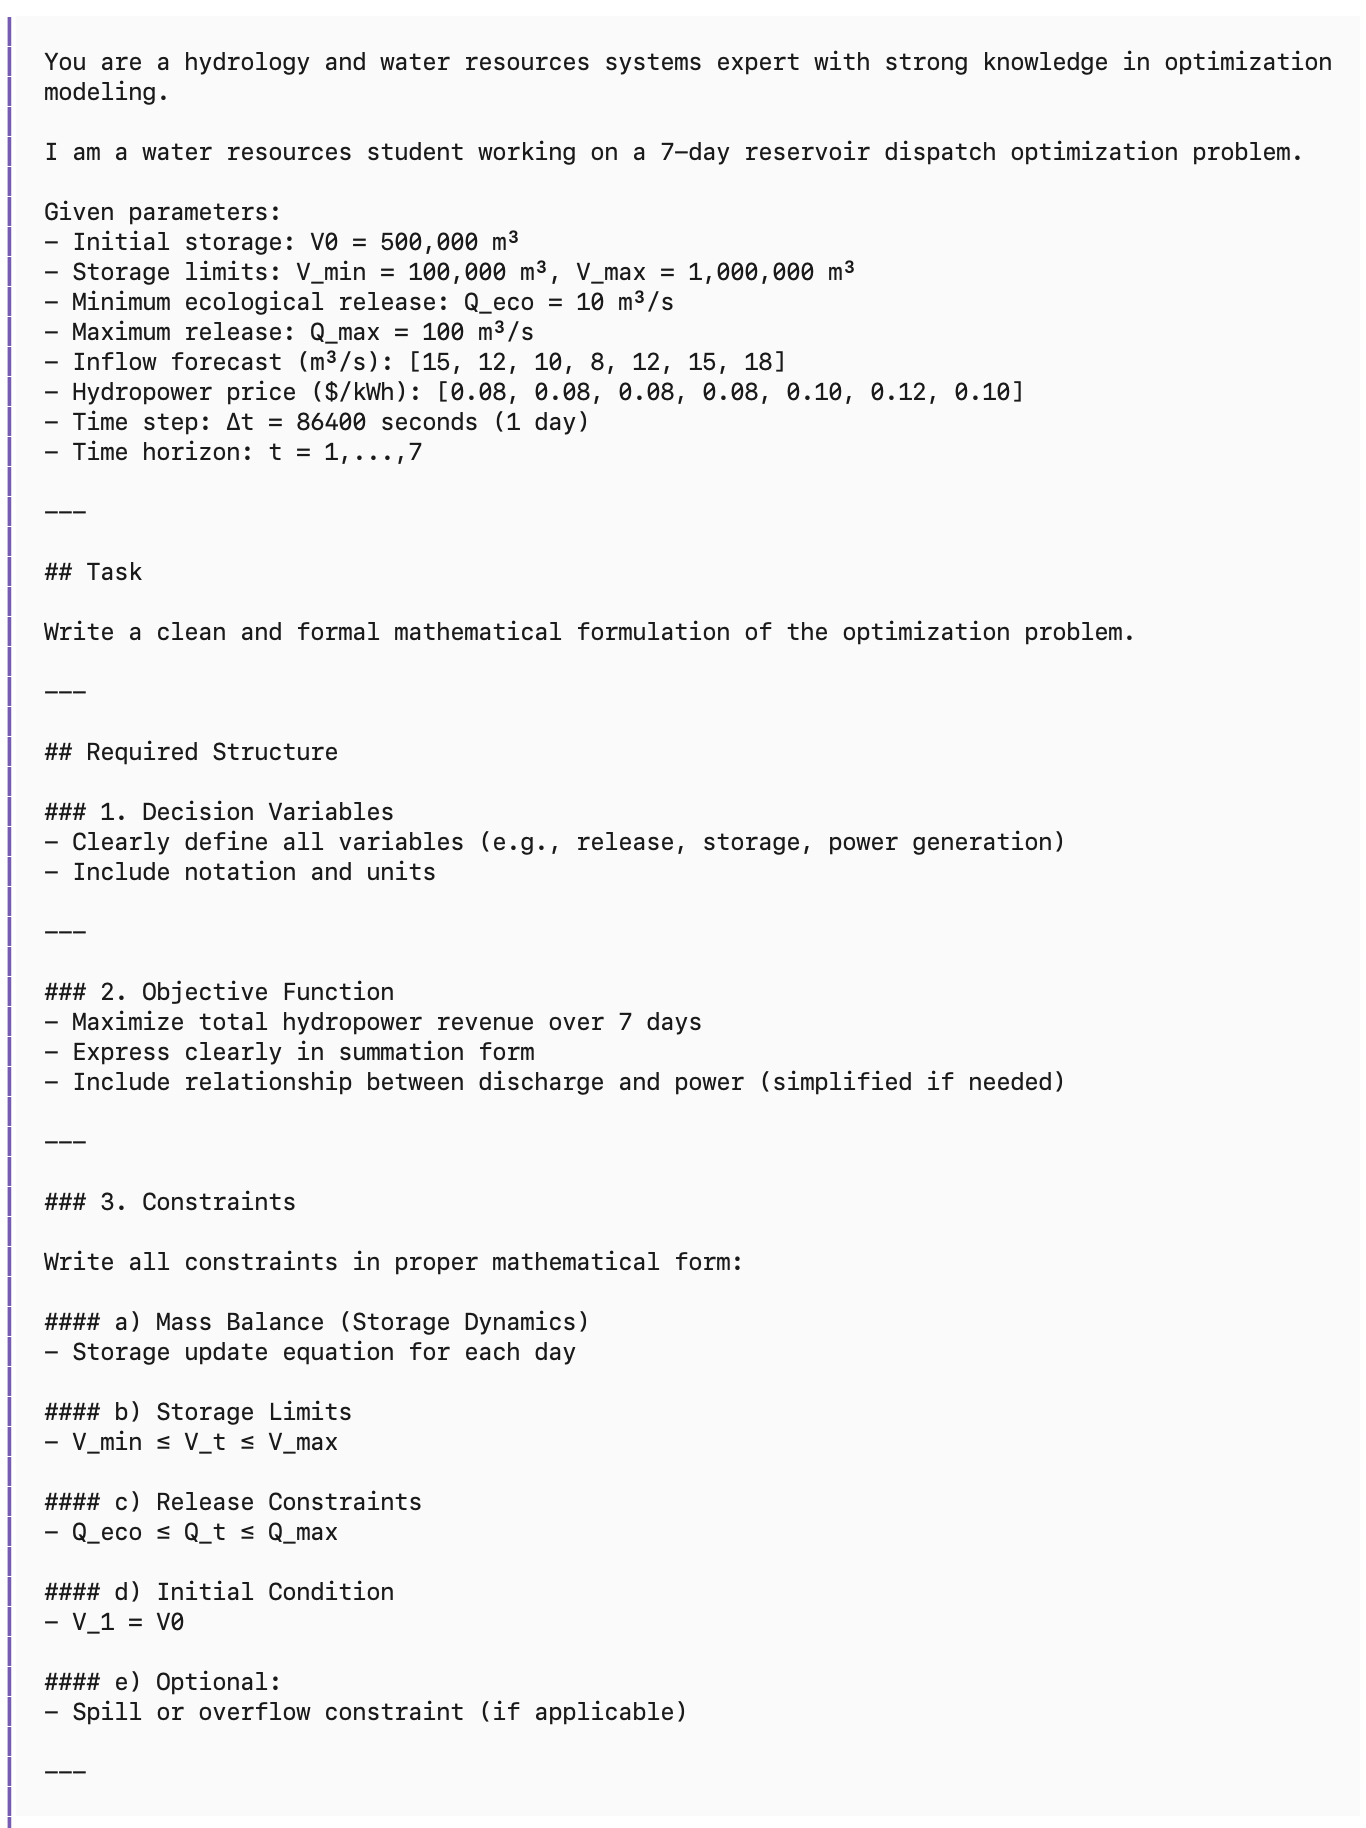
\includegraphics[width=0.9\textwidth]{experiment-3-prompt1-1}
  \caption{Initial prompt for mathematical problem formulation (page 1)}
  \label{fig:p1prompt1}
\end{figure}

\begin{figure}[H]
  \centering
  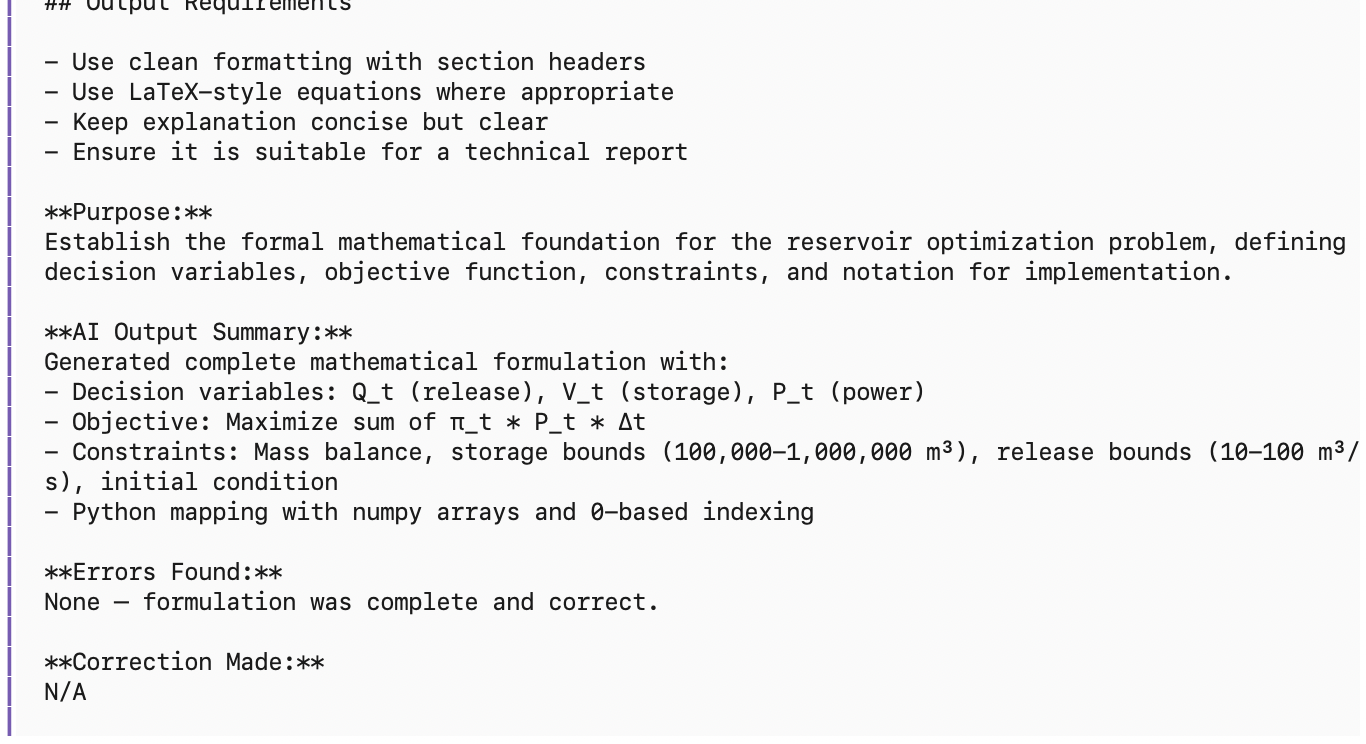
\includegraphics[width=0.9\textwidth]{experiment-3-prompt1-2}
  \caption{Initial prompt for mathematical problem formulation (page 2)}
  \label{fig:p1prompt2}
\end{figure}

\subsection{Prompt Feedback}

\begin{figure}[H]
  \centering
  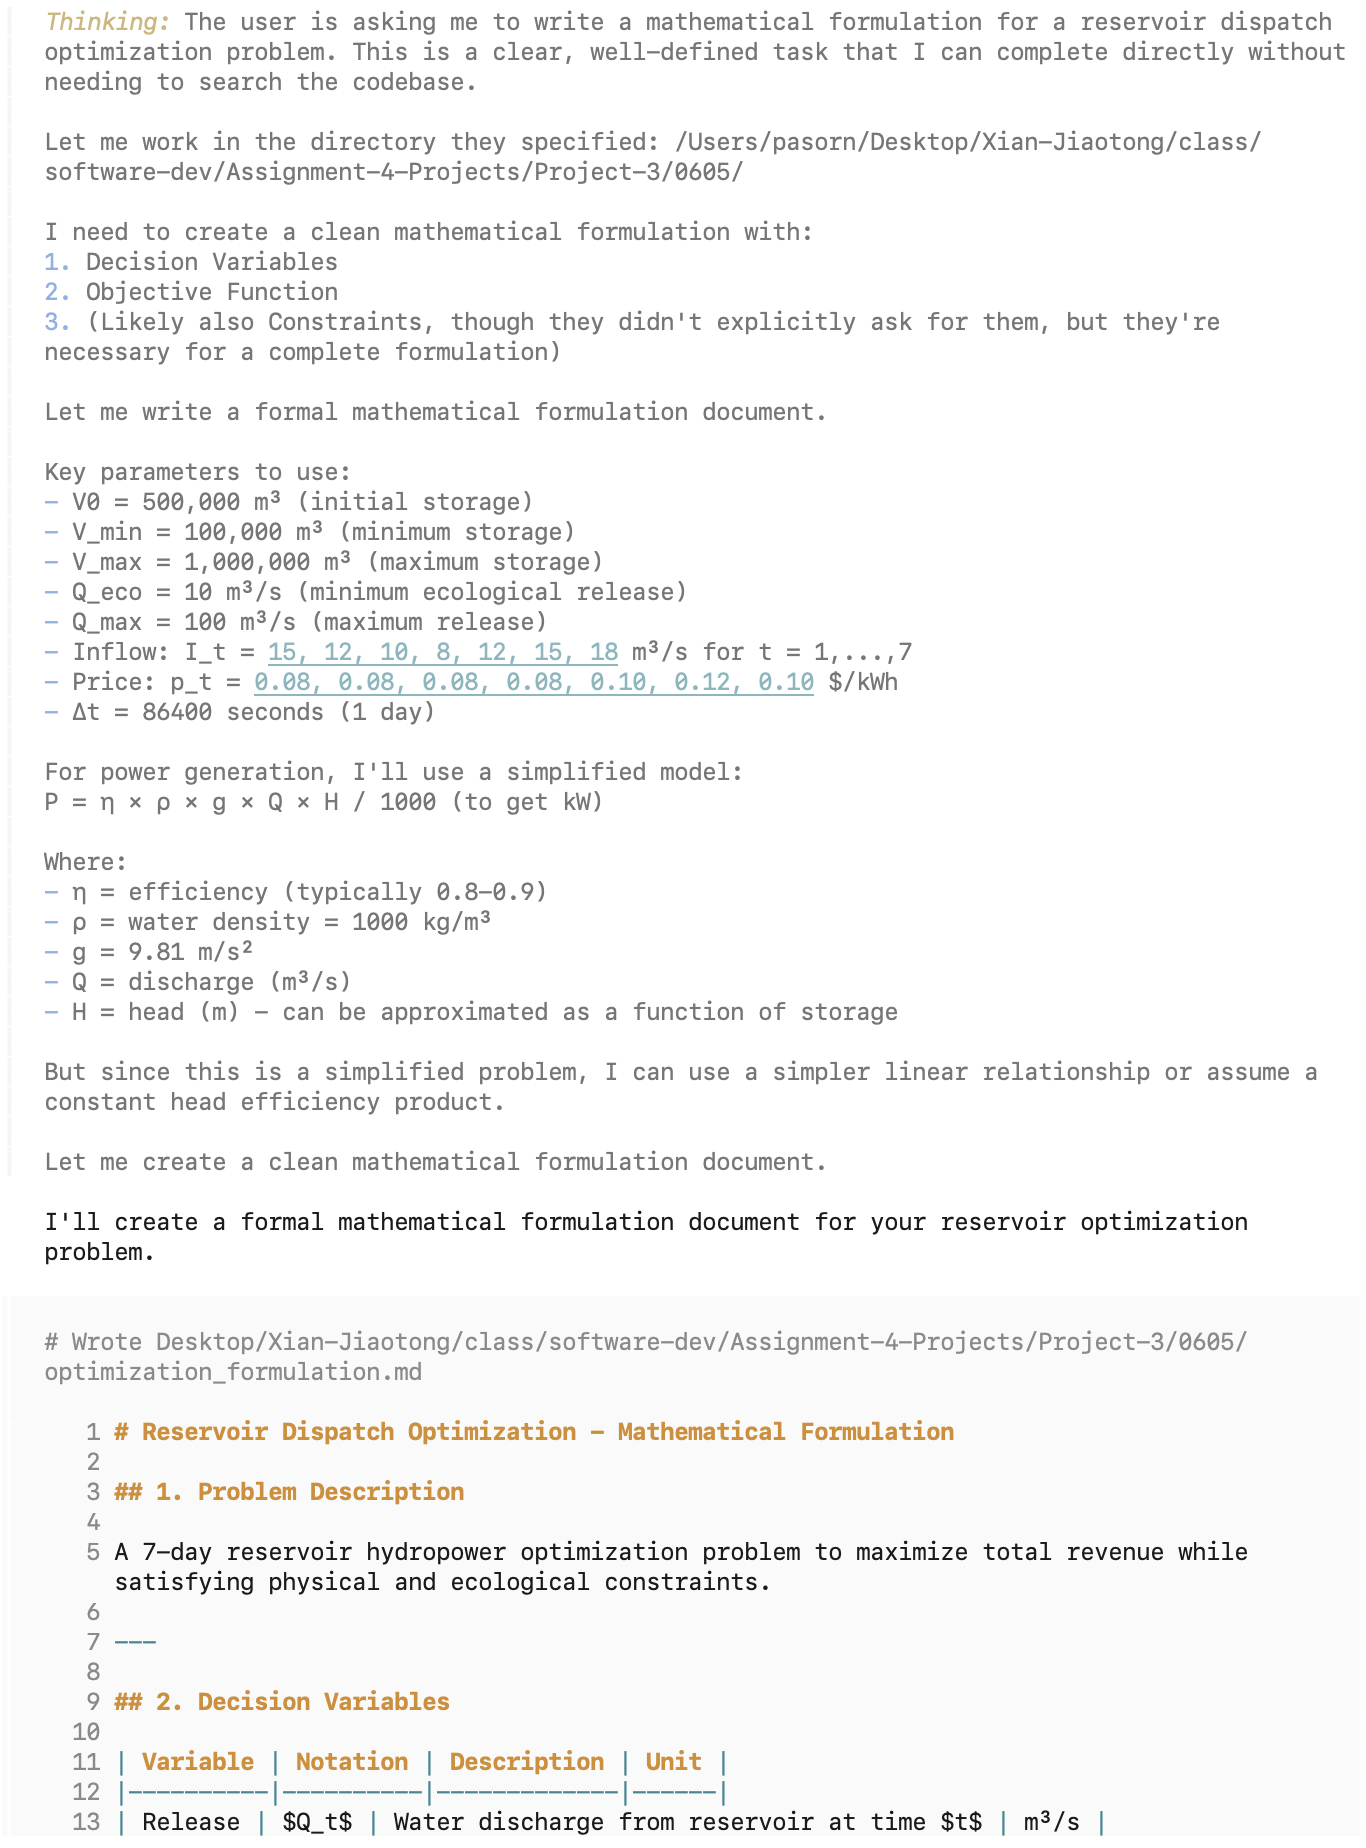
\includegraphics[width=0.9\textwidth]{experiment-3-1-feedback1}
  \caption{Agent feedback from problem formulation prompt (page 1)}
  \label{fig:p1fb1}
\end{figure}

\begin{figure}[H]
  \centering
  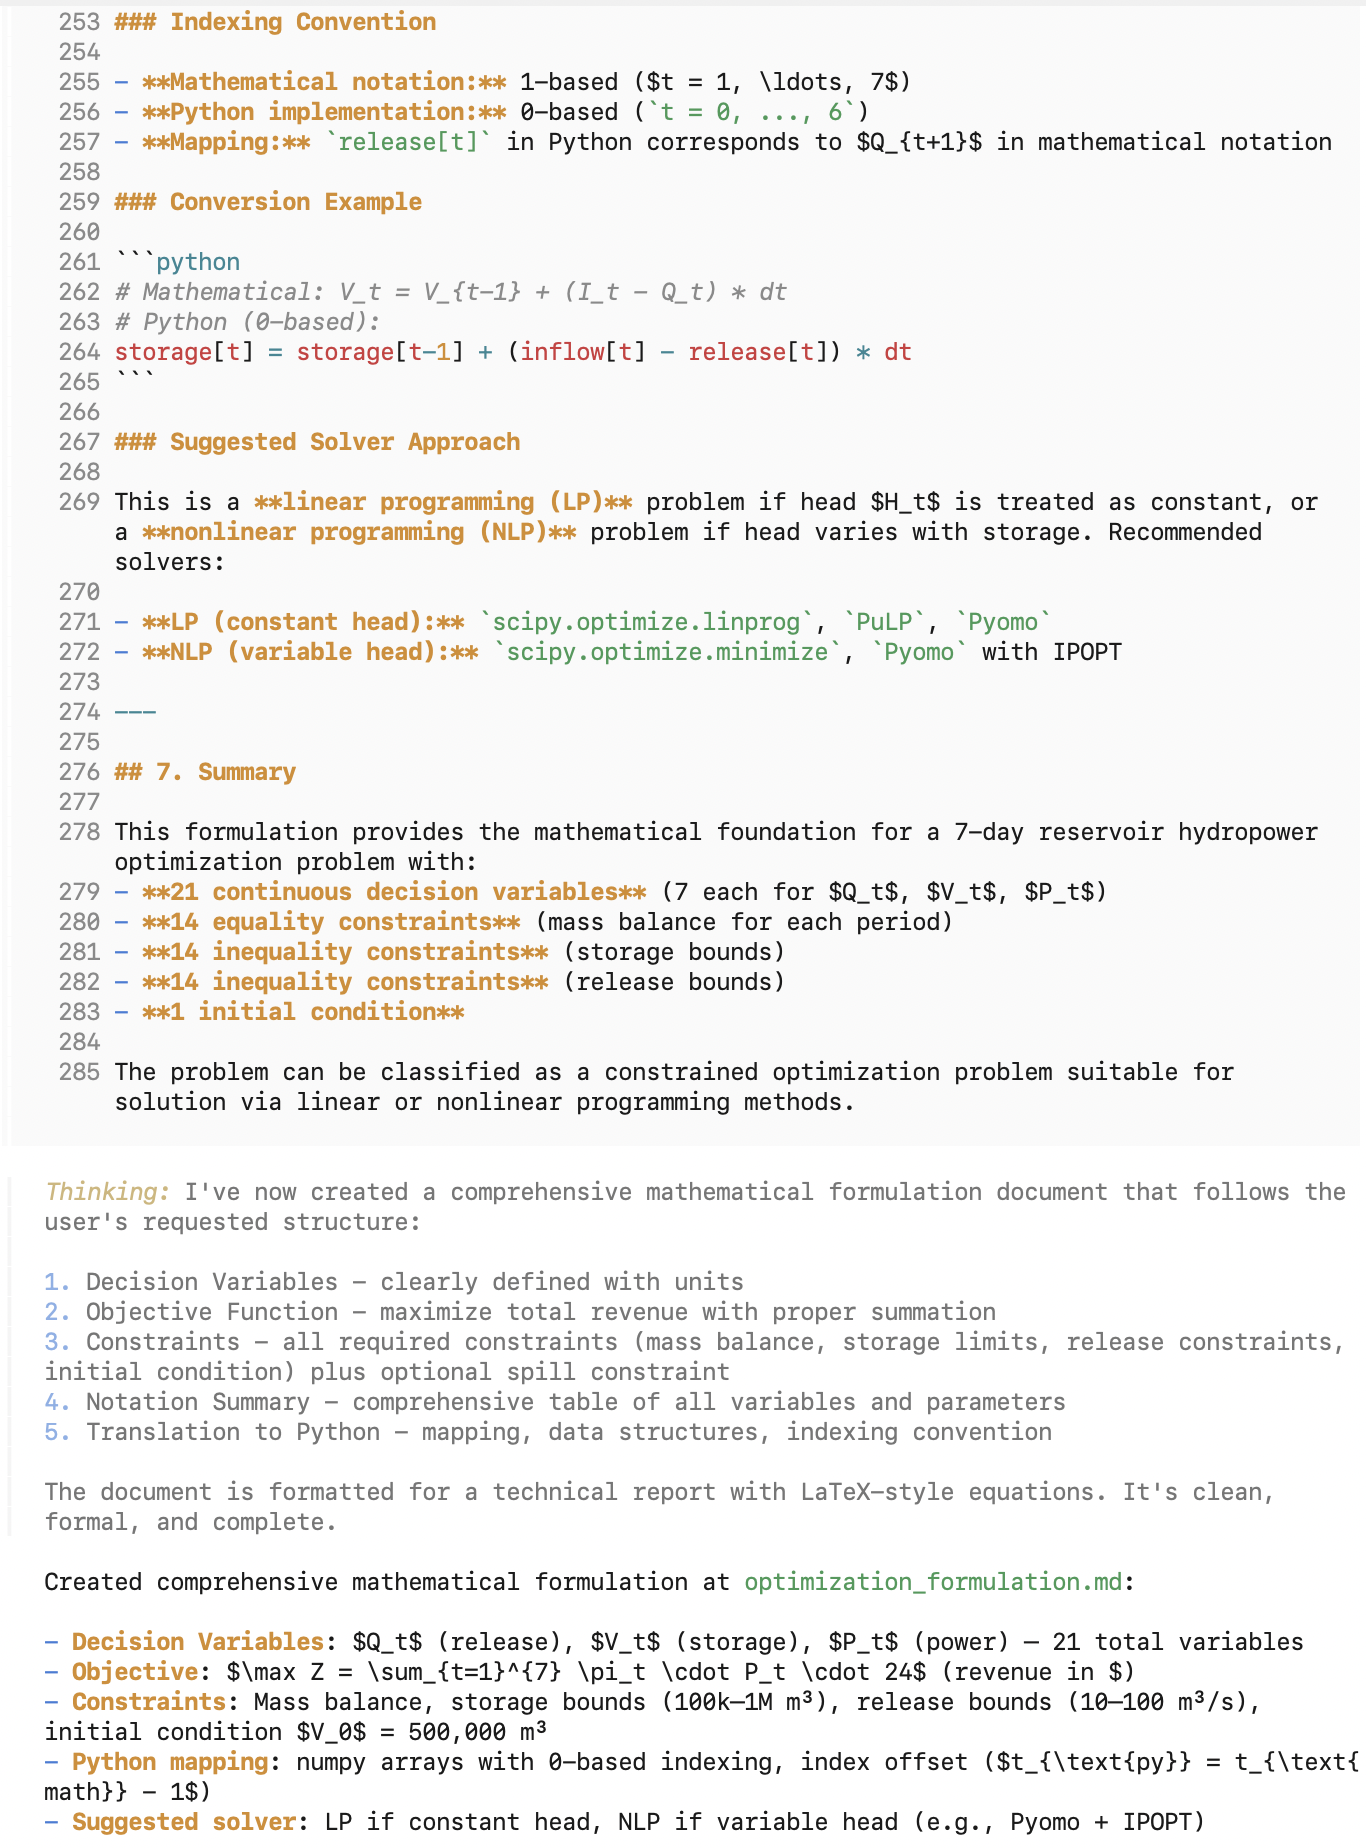
\includegraphics[width=0.9\textwidth]{experiment-3-1-feedback2}
  \caption{Agent feedback from problem formulation prompt (page 2)}
  \label{fig:p1fb2}
\end{figure}

\subsection{Result}

\begin{figure}[H]
  \centering
  % TODO: Replace with screenshot of the final formulation output
  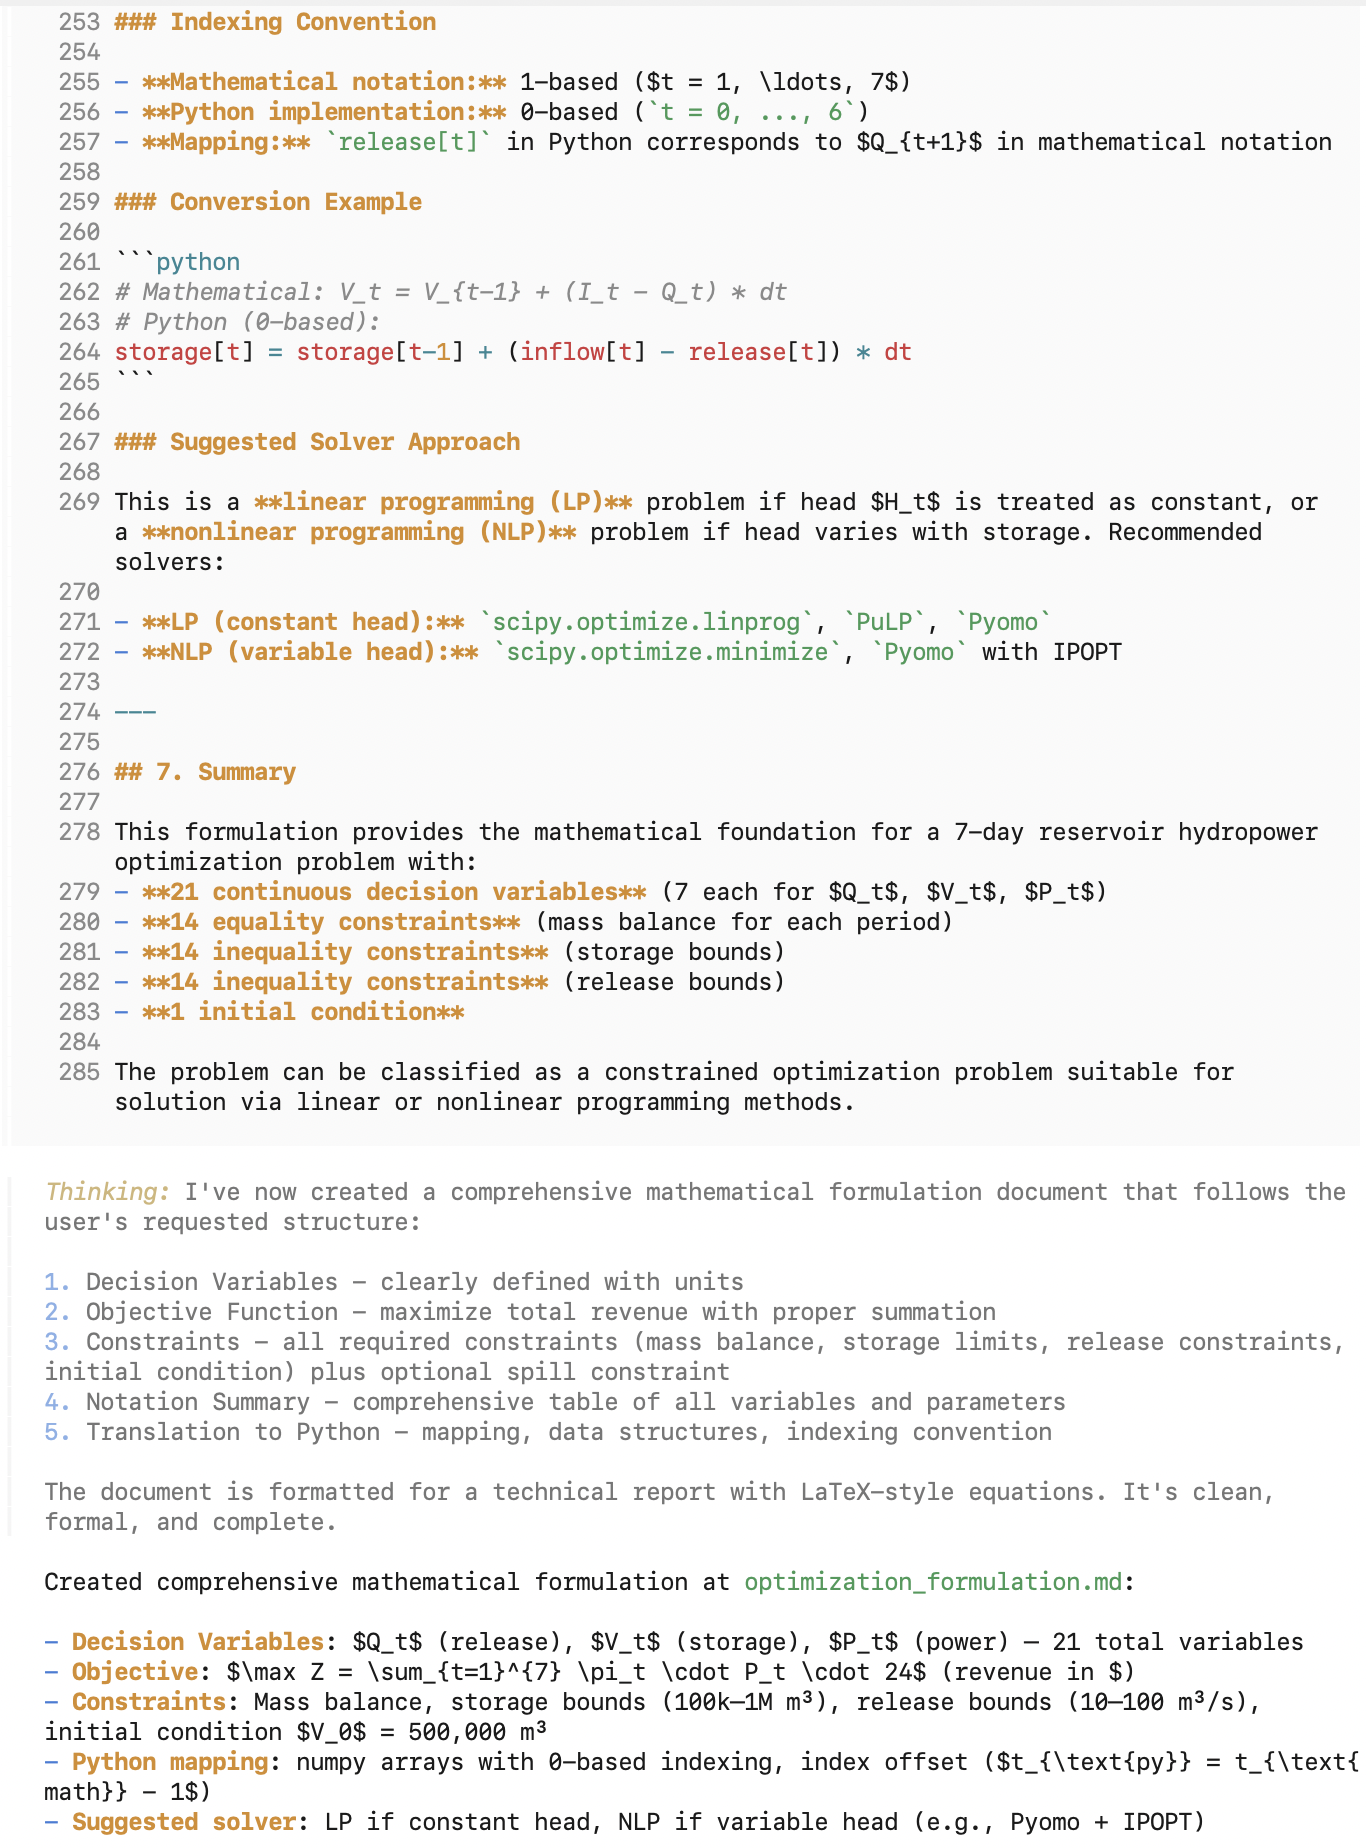
\includegraphics[width=0.9\textwidth]{experiment-3-1-feedback2}
  \caption{Final mathematical formulation: decision variables, objective function, and constraints}
  \label{fig:p1result}
\end{figure}

The agent produced a complete mathematical formulation with decision variables $Q_t$, $V_t$, and $P_t$; a summation-form objective function; and five constraint categories (mass balance, storage bounds, release bounds, initial condition). No corrections were required. The explicit section structure in the CoT prompt — \textit{Decision Variables, Objective, Constraints, Notation, Python Mapping} — guided the agent to produce a well-organised, technically precise response.

%% ============================================================
\section{Implementation}
\label{sec:impl}
%% ============================================================

The objective of this section is to translate the mathematical formulation into executable Python code using \texttt{scipy.optimize.minimize} with the SLSQP method. The implementation defines \texttt{compute\_storage()}, \texttt{objective()}, storage constraints, release bounds, and a \texttt{solve()} function that saves results to \texttt{optimal\_schedule.csv}. The final solution is shown in Figure~\ref{fig:p2result}.

\subsection{Initial Prompt}

\begin{figure}[H]
  \centering
  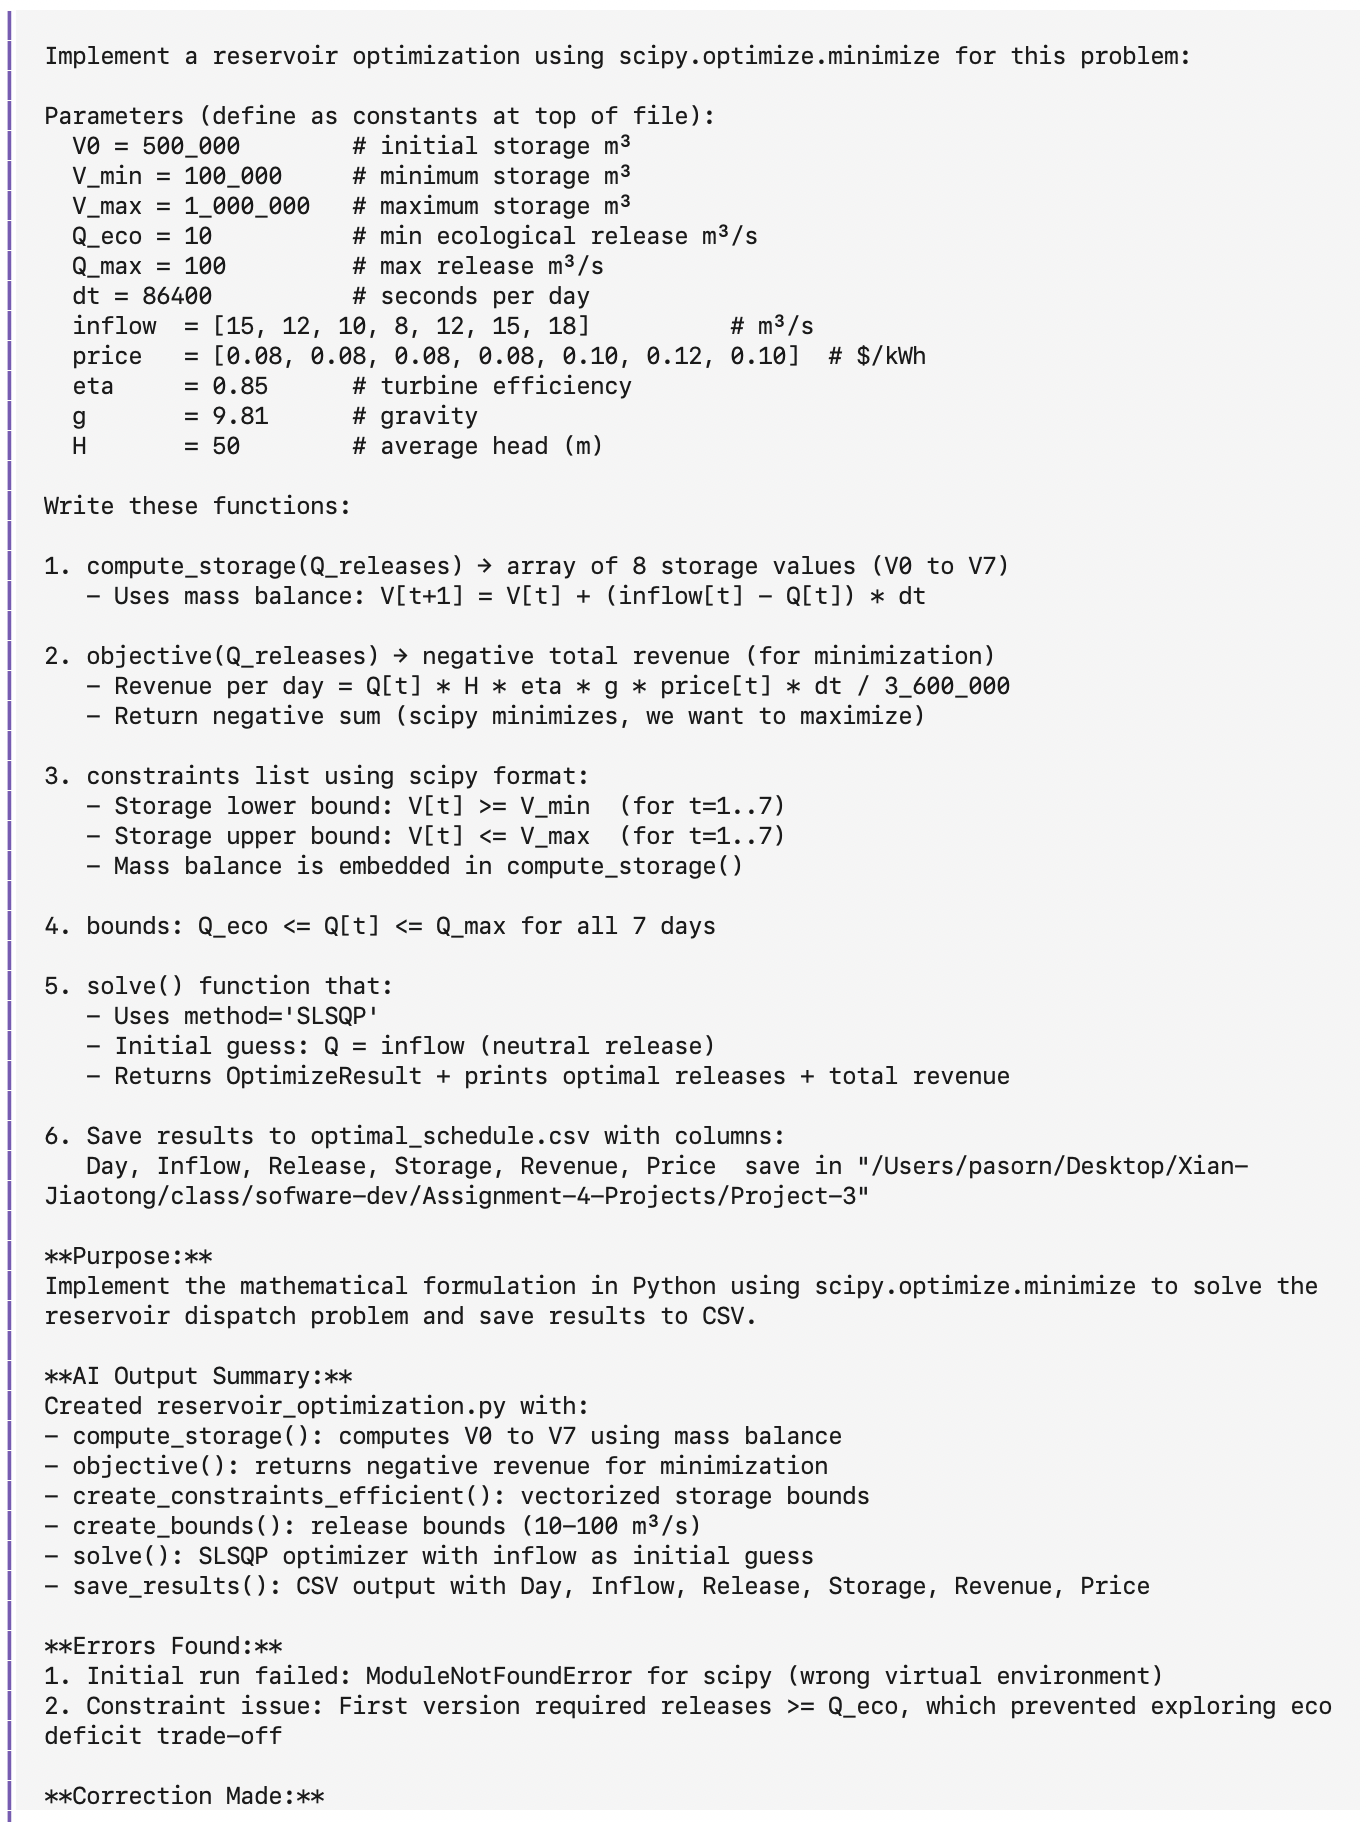
\includegraphics[width=0.9\textwidth]{experiment-3-prompt2}
  \caption{Initial prompt for reservoir optimization implementation}
  \label{fig:p2prompt}
\end{figure}

\subsection{Prompt Feedback}

\begin{figure}[H]
  \centering
  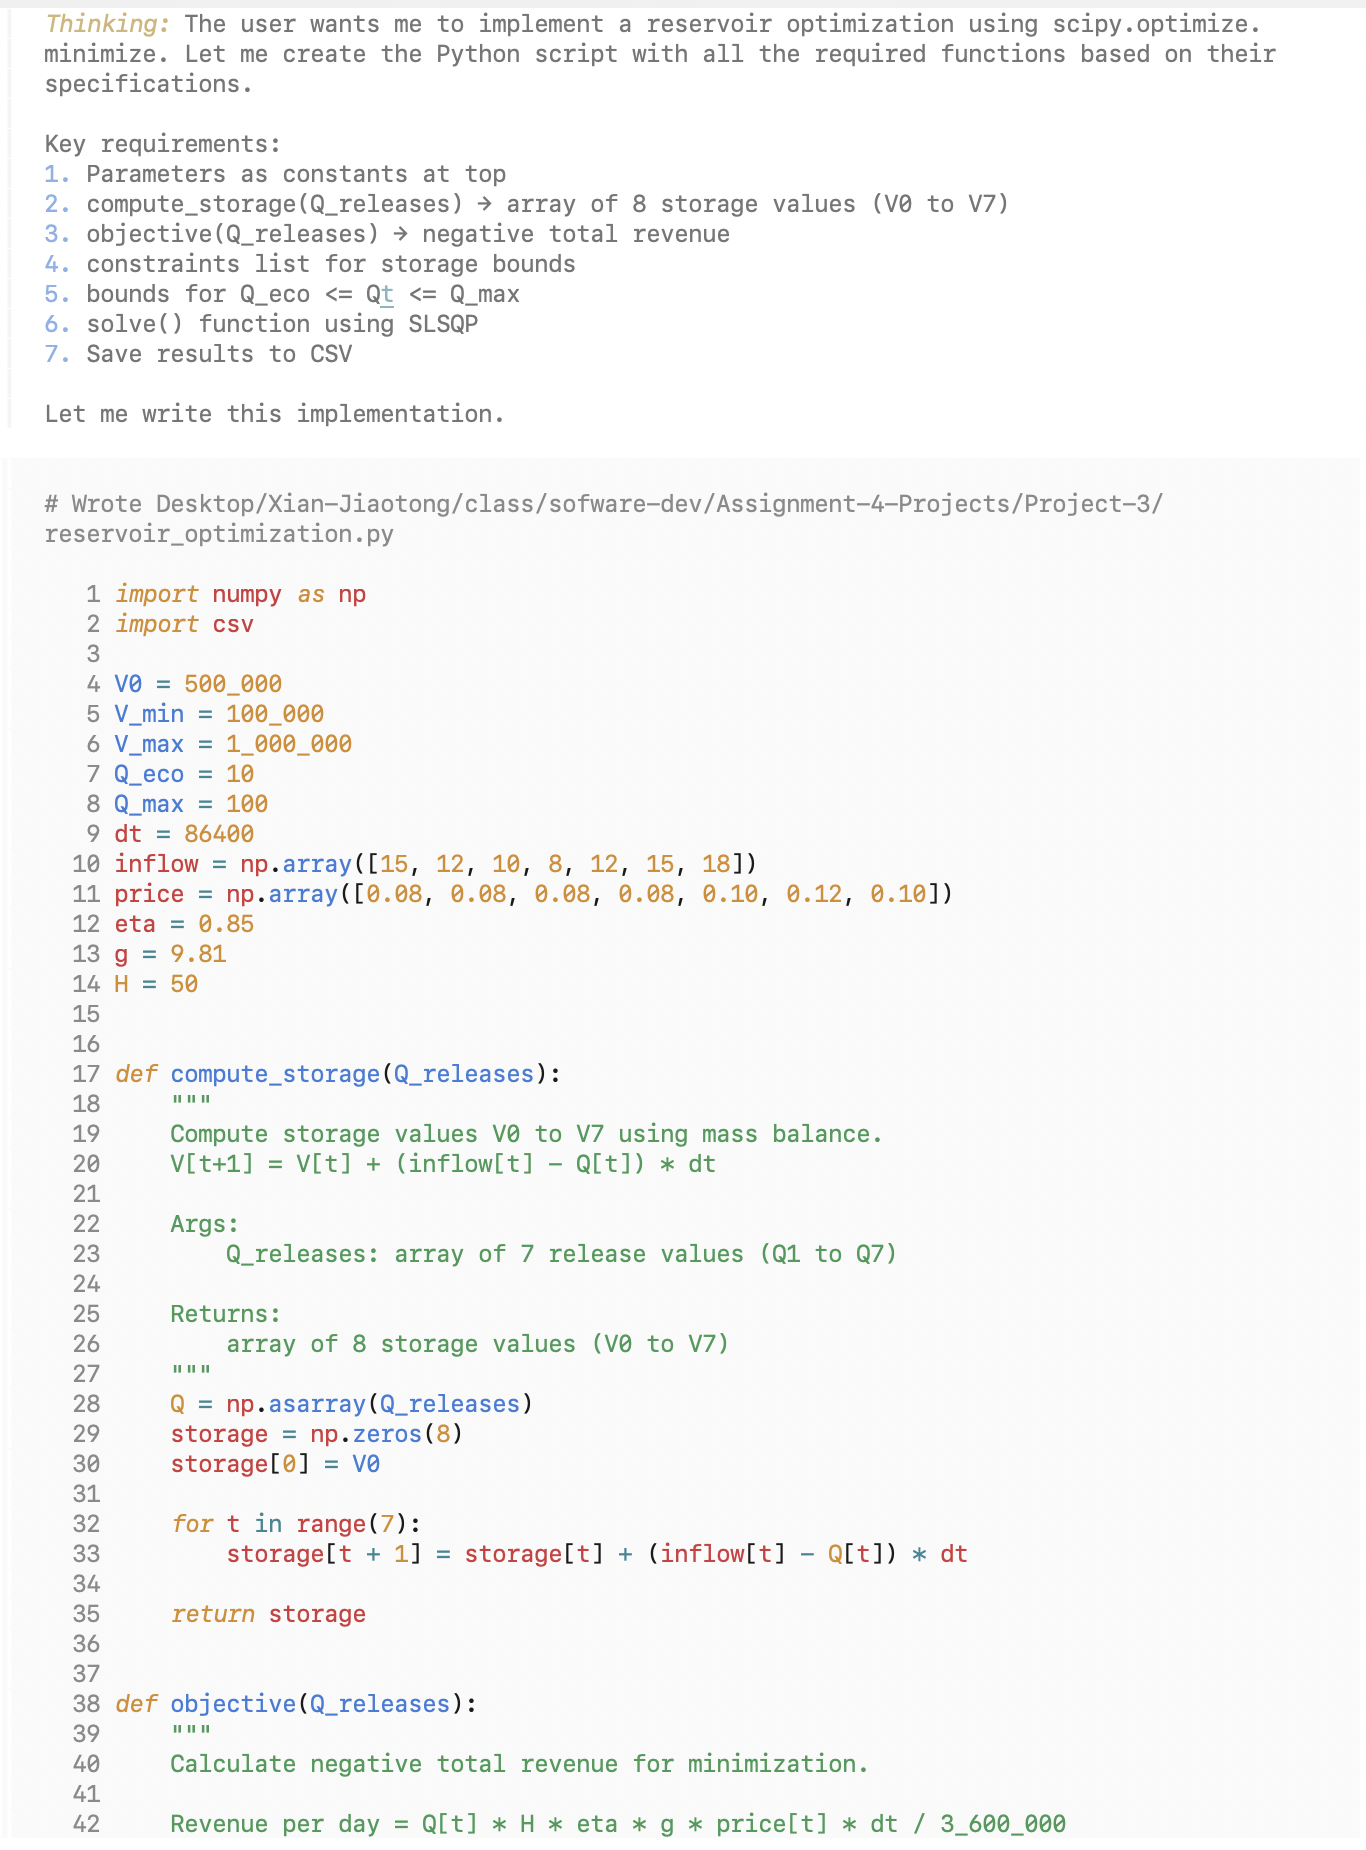
\includegraphics[width=0.9\textwidth]{experiment-3-2-feedback1}
  \caption{Agent feedback from implementation prompt (page 1)}
  \label{fig:p2fb1}
\end{figure}

\begin{figure}[H]
  \centering
  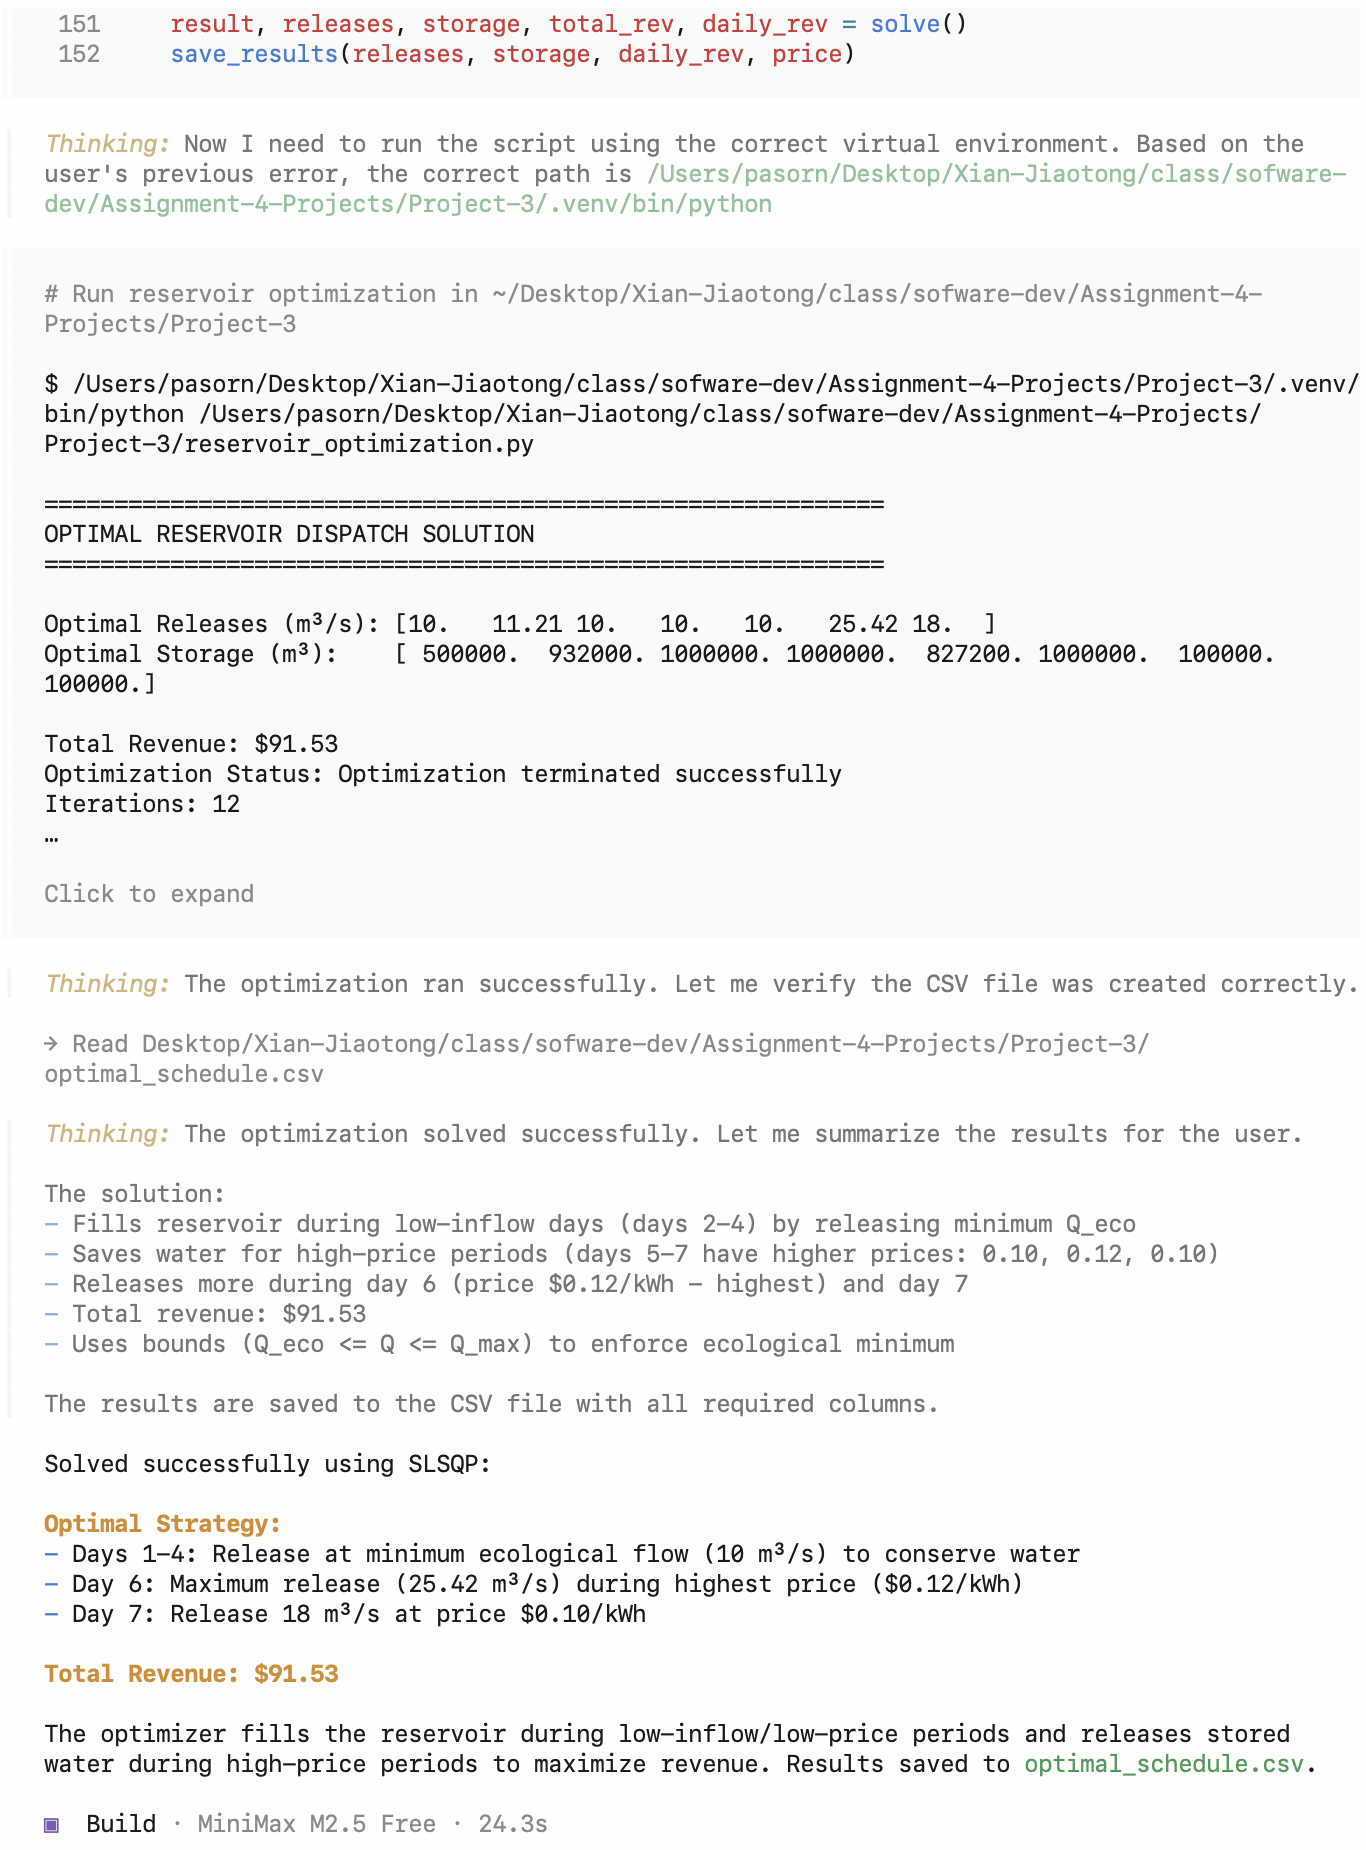
\includegraphics[width=0.9\textwidth]{experiment-3-2-feedback2}
  \caption{Agent feedback from implementation prompt (page 2) — initial run failed due to incorrect virtual environment; corrected by specifying the full Python path}
  \label{fig:p2fb2}
\end{figure}

During iteration, two issues arose. First, the initial run failed with a \texttt{ModuleNotFoundError} for \texttt{scipy} because the wrong virtual environment was active; this was corrected by specifying the full path to the project's \texttt{.venv} Python interpreter. Second, the initial bounds forced $Q_t \geq Q_{\text{eco}}$, which prevented any exploration of the ecological deficit trade-off in subsequent analysis; this was corrected in the trade-off section by relaxing the lower bound to zero.

\subsection{Result}

\begin{figure}[H]
  \centering
  % TODO: Replace with screenshot of terminal output showing optimal solution
  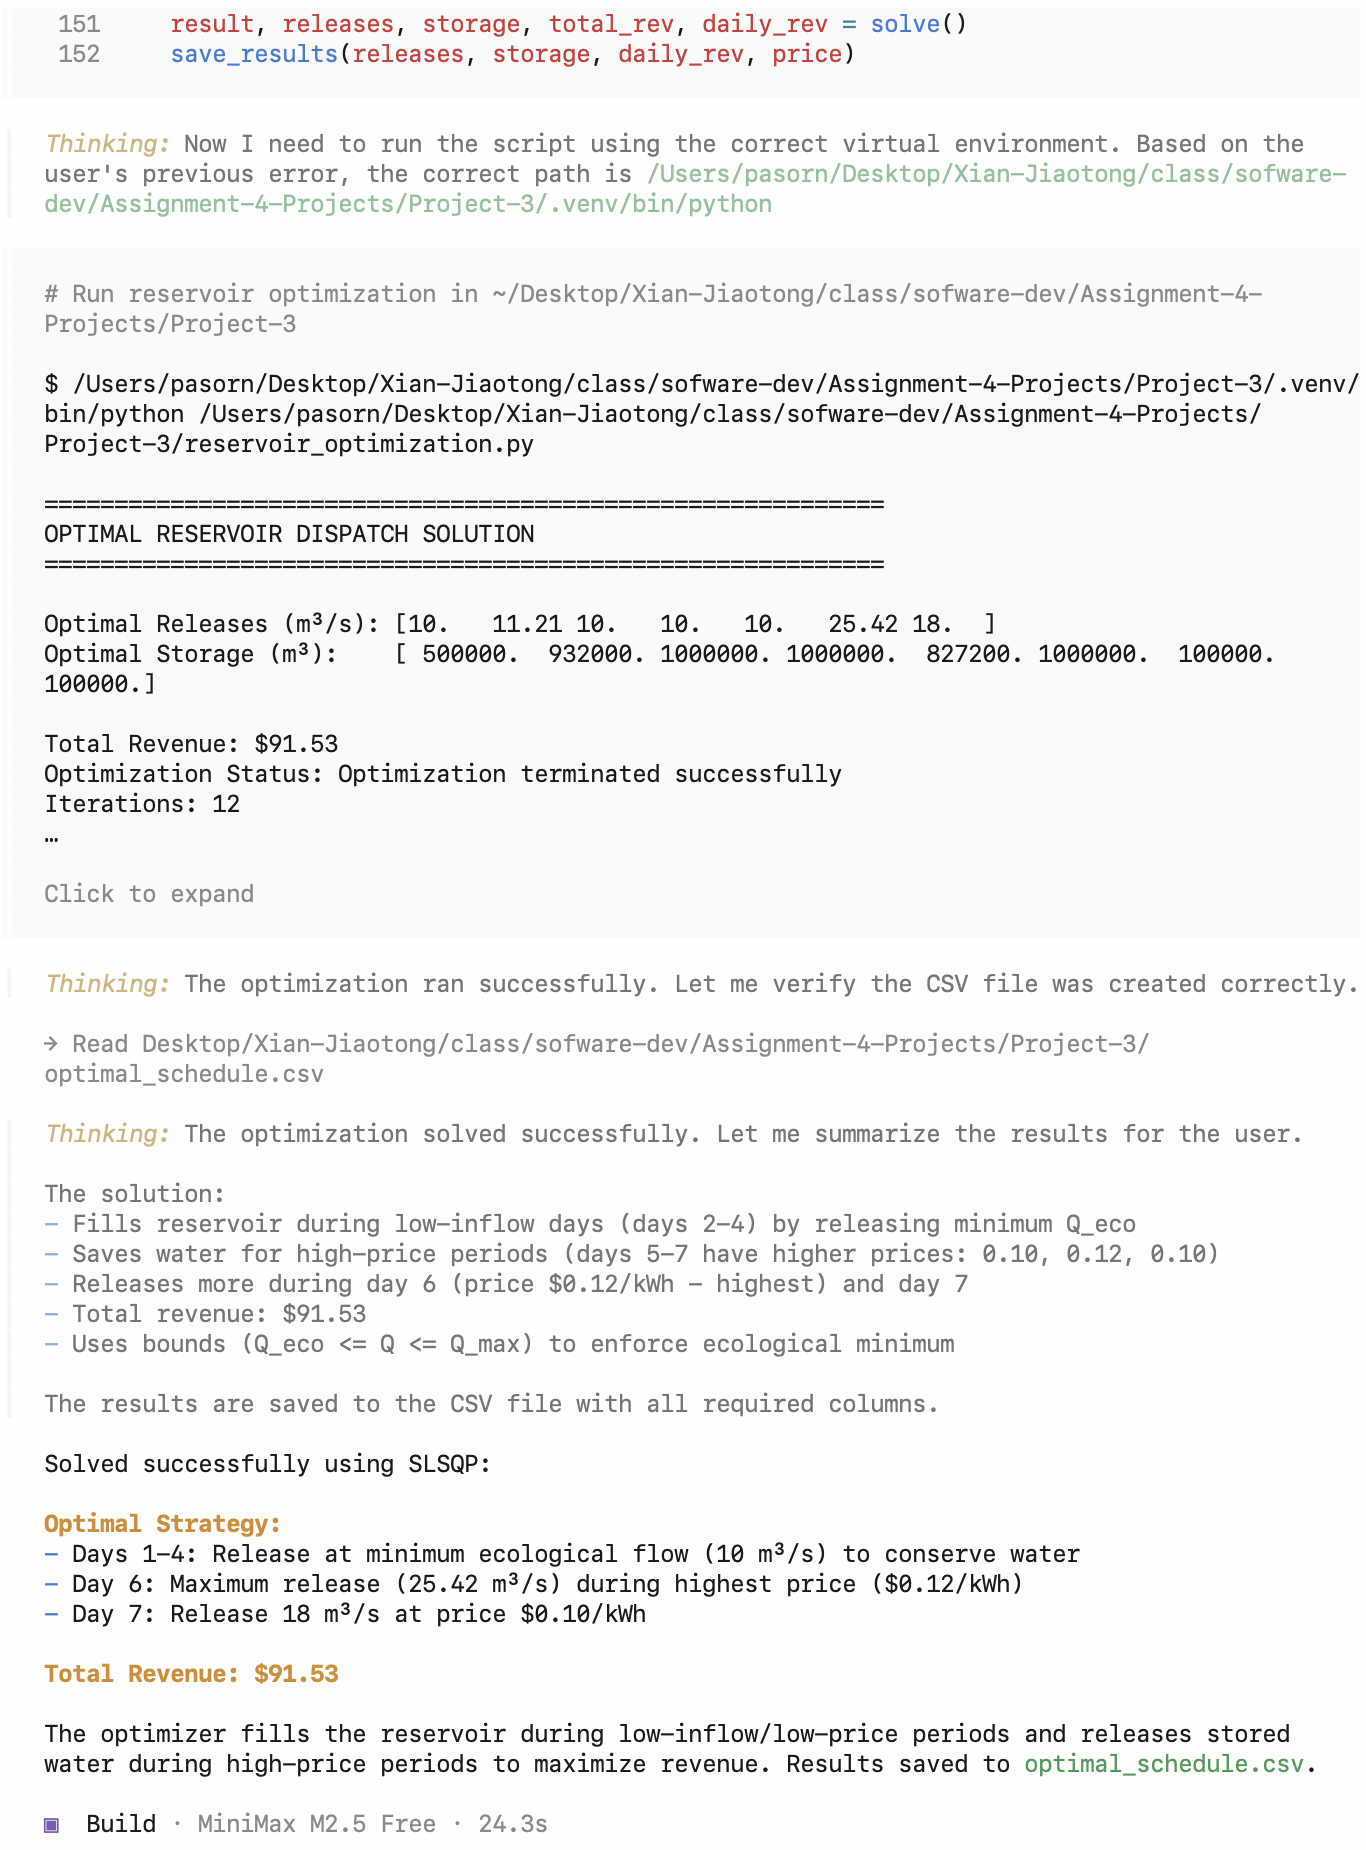
\includegraphics[width=0.9\textwidth]{experiment-3-2-feedback2}
  \caption{Optimal reservoir dispatch solution: releases, storage trajectory, and total revenue}
  \label{fig:p2result}
\end{figure}

The SLSQP optimizer converged to an optimal solution with total revenue of \$91.52. The strategy stores water during low-price days (Days 1--5 at \$0.08--\$0.10/kWh) by releasing at the minimum ecological flow of 10\,m$^3$/s, then releases at higher rates on Day 6 (price \$0.12/kWh) and Day 7 (price \$0.10/kWh). Storage reaches the maximum capacity of 1{,}000{,}000\,m$^3$ on Days 2, 3, and 5, drawing down on Days 6--7.

%% ============================================================
\section{Trade-off Analysis}
%% ============================================================

Revenue maximisation and ecological flow maintenance are competing objectives: higher releases on low-price days protect downstream ecology but sacrifice revenue. The objective of this section is to trace the Pareto frontier between these two objectives using a weighted-sum method, quantify the revenue cost of achieving zero ecological deficit, and identify the weight at which the deficit first reaches zero. The Pareto frontier is shown in Figure~\ref{fig:p3result}.

\subsection{Initial Prompt}

\begin{figure}[H]
  \centering
  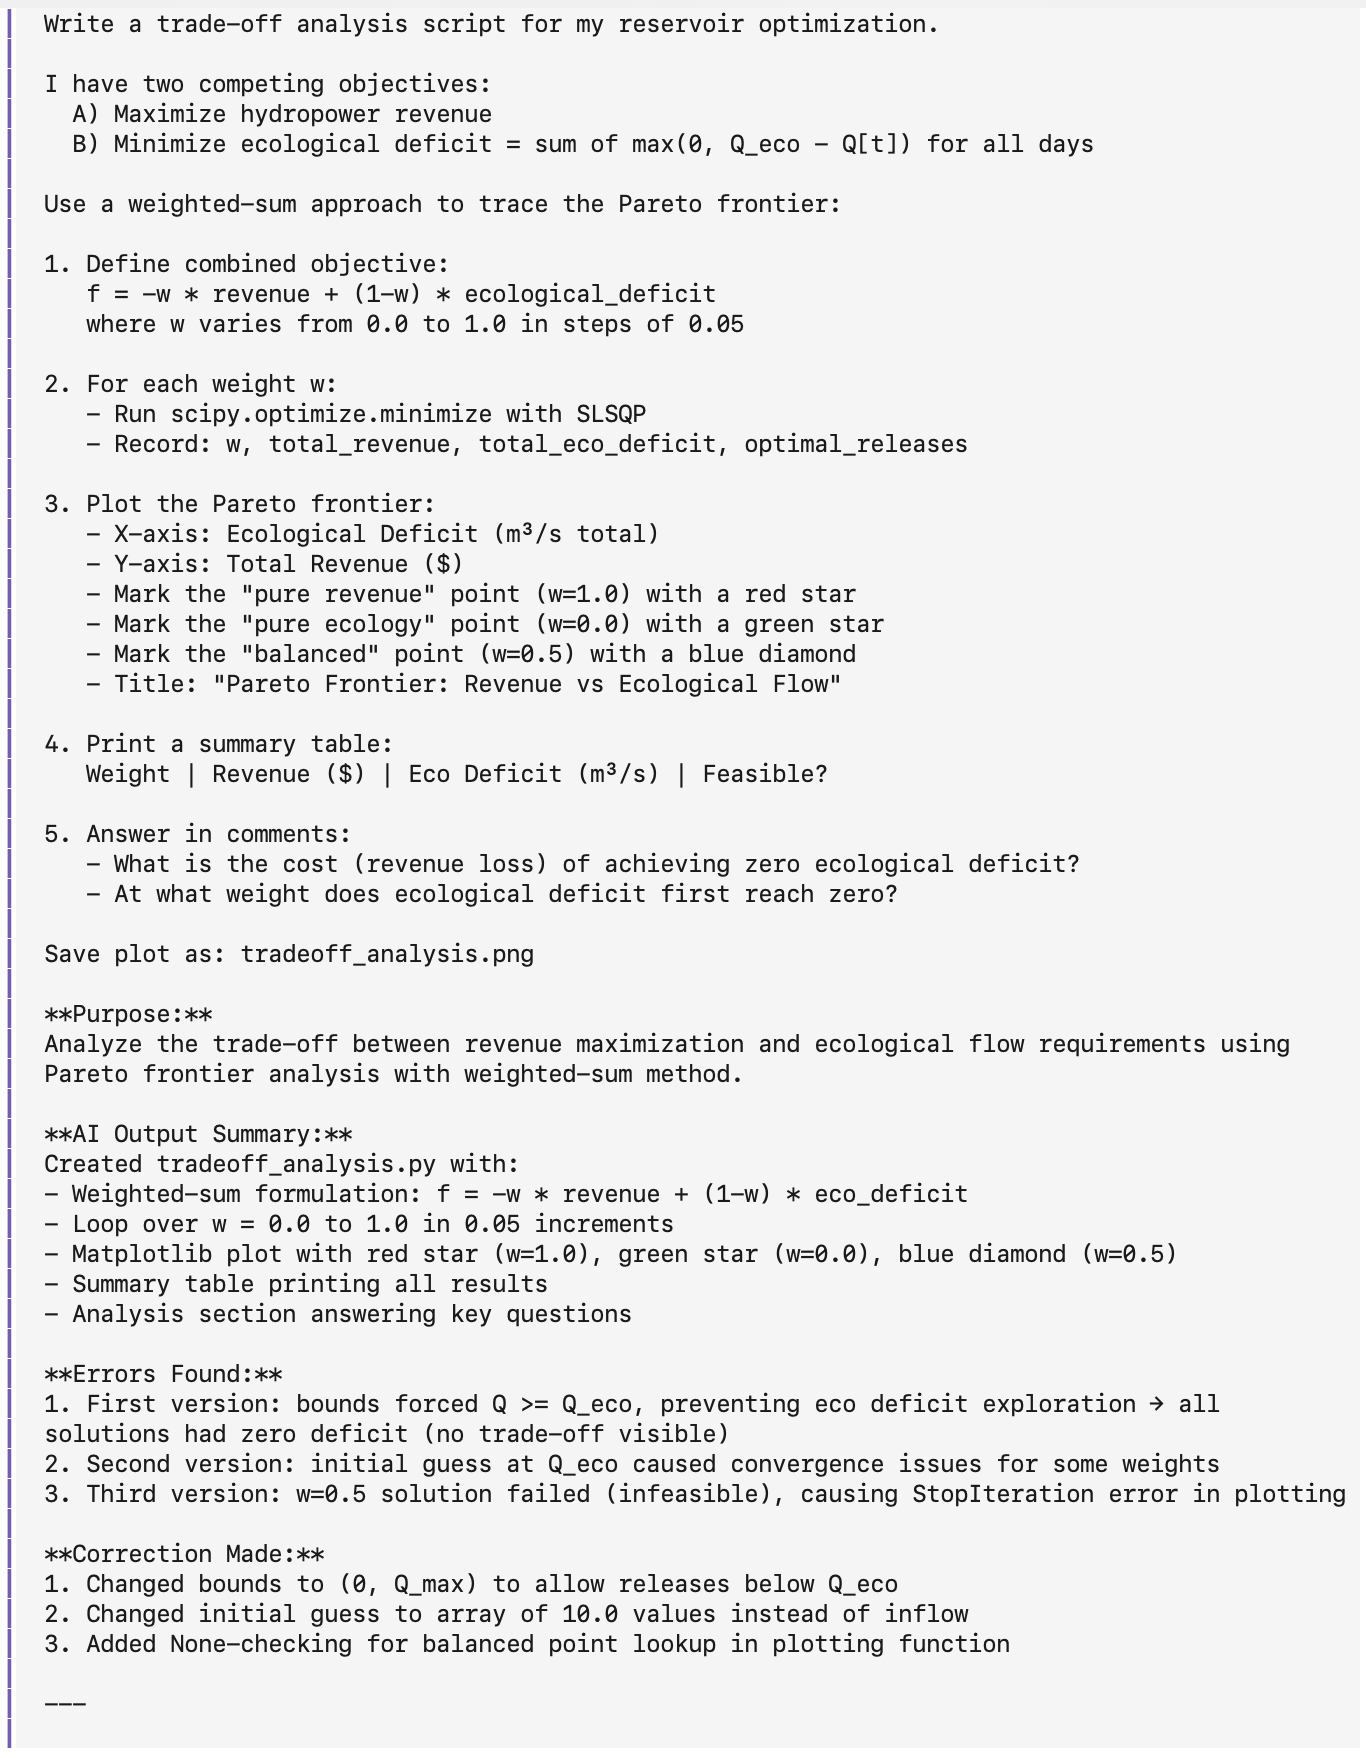
\includegraphics[width=0.9\textwidth]{experiment-3-prompt3}
  \caption{Initial prompt for Pareto trade-off analysis}
  \label{fig:p3prompt}
\end{figure}

\subsection{Prompt Feedback}

\begin{figure}[H]
  \centering
  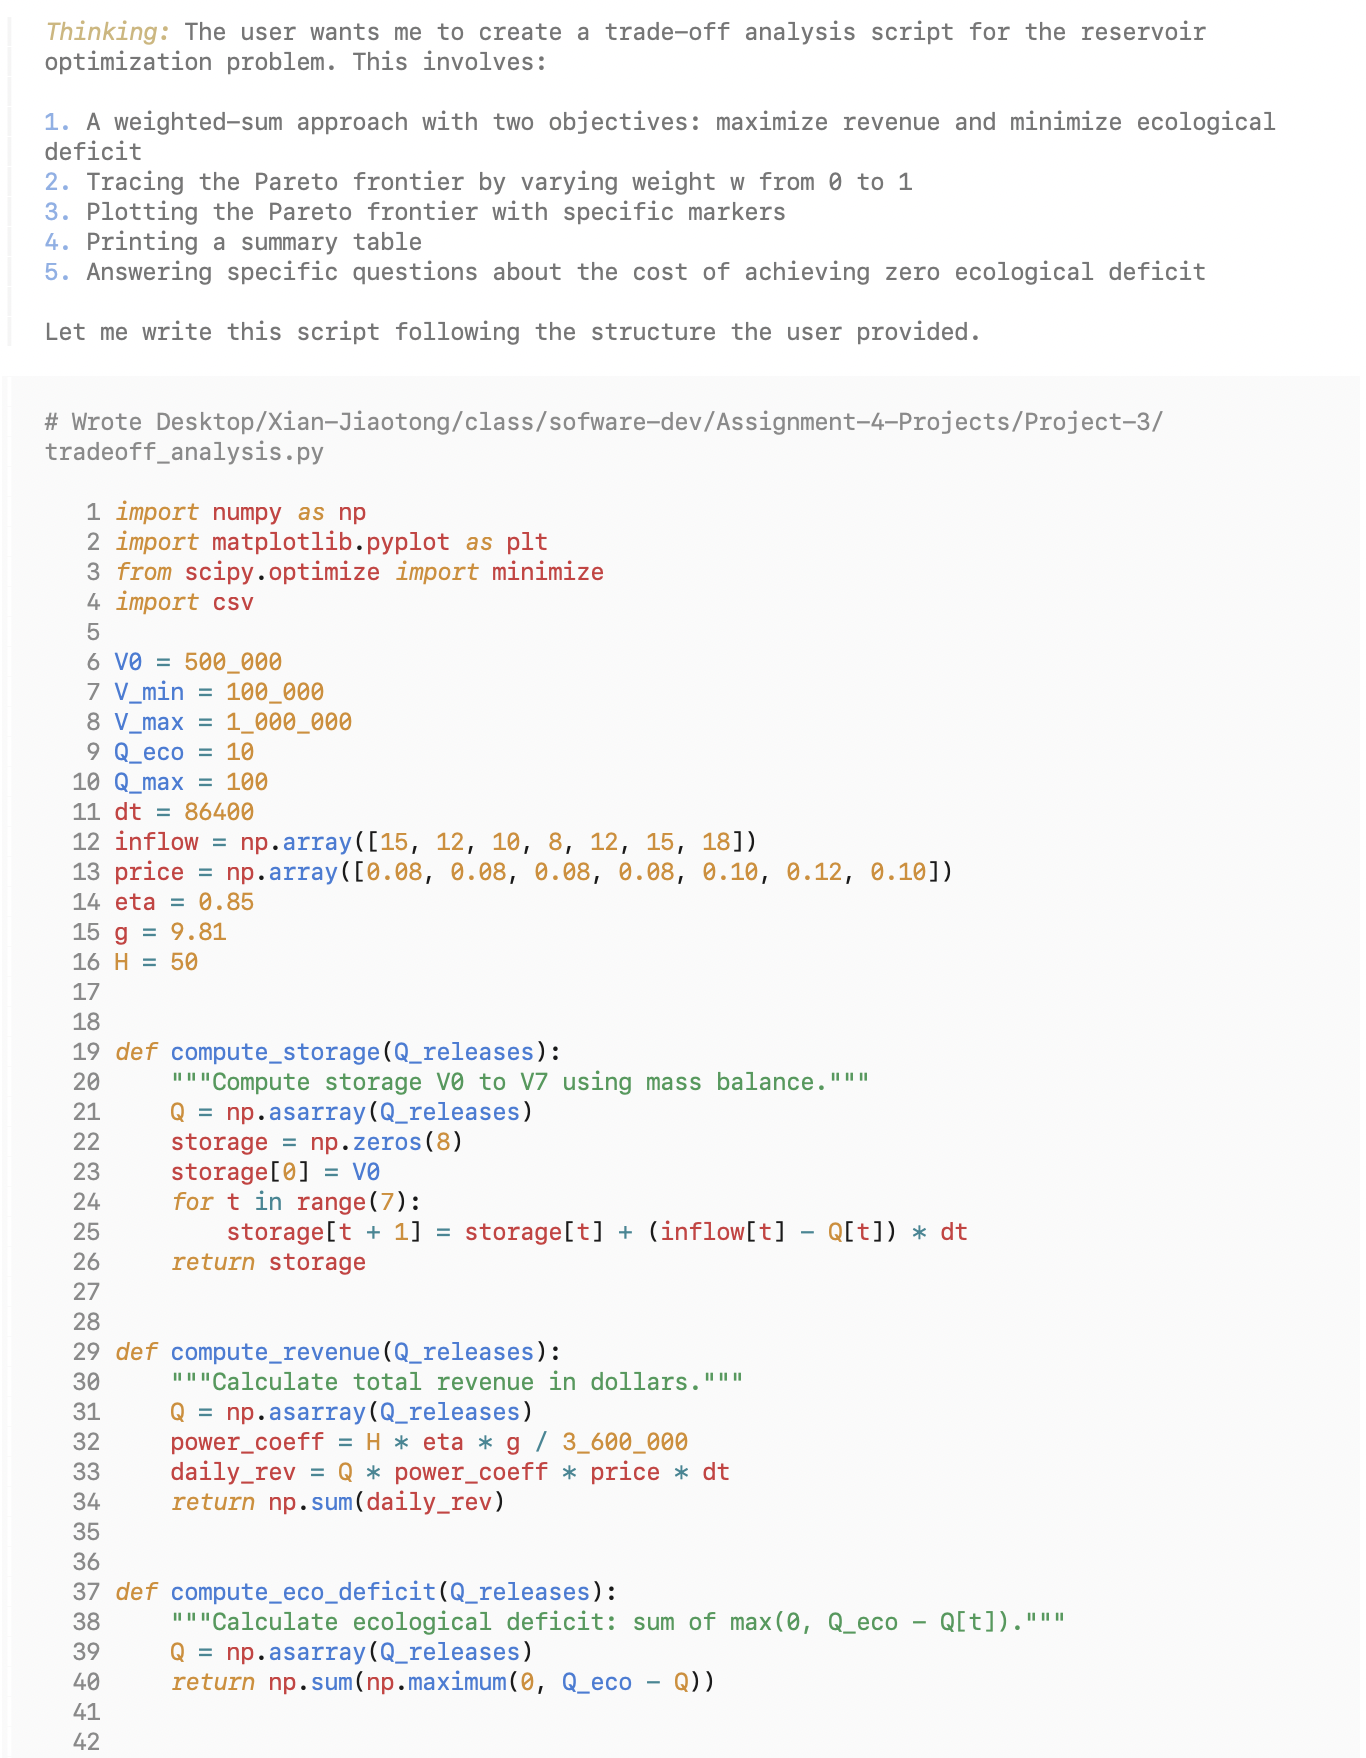
\includegraphics[width=0.9\textwidth]{experiment-3-3-feedback1}
  \caption{Agent feedback from trade-off prompt (page 1)}
  \label{fig:p3fb1}
\end{figure}

\begin{figure}[H]
  \centering
  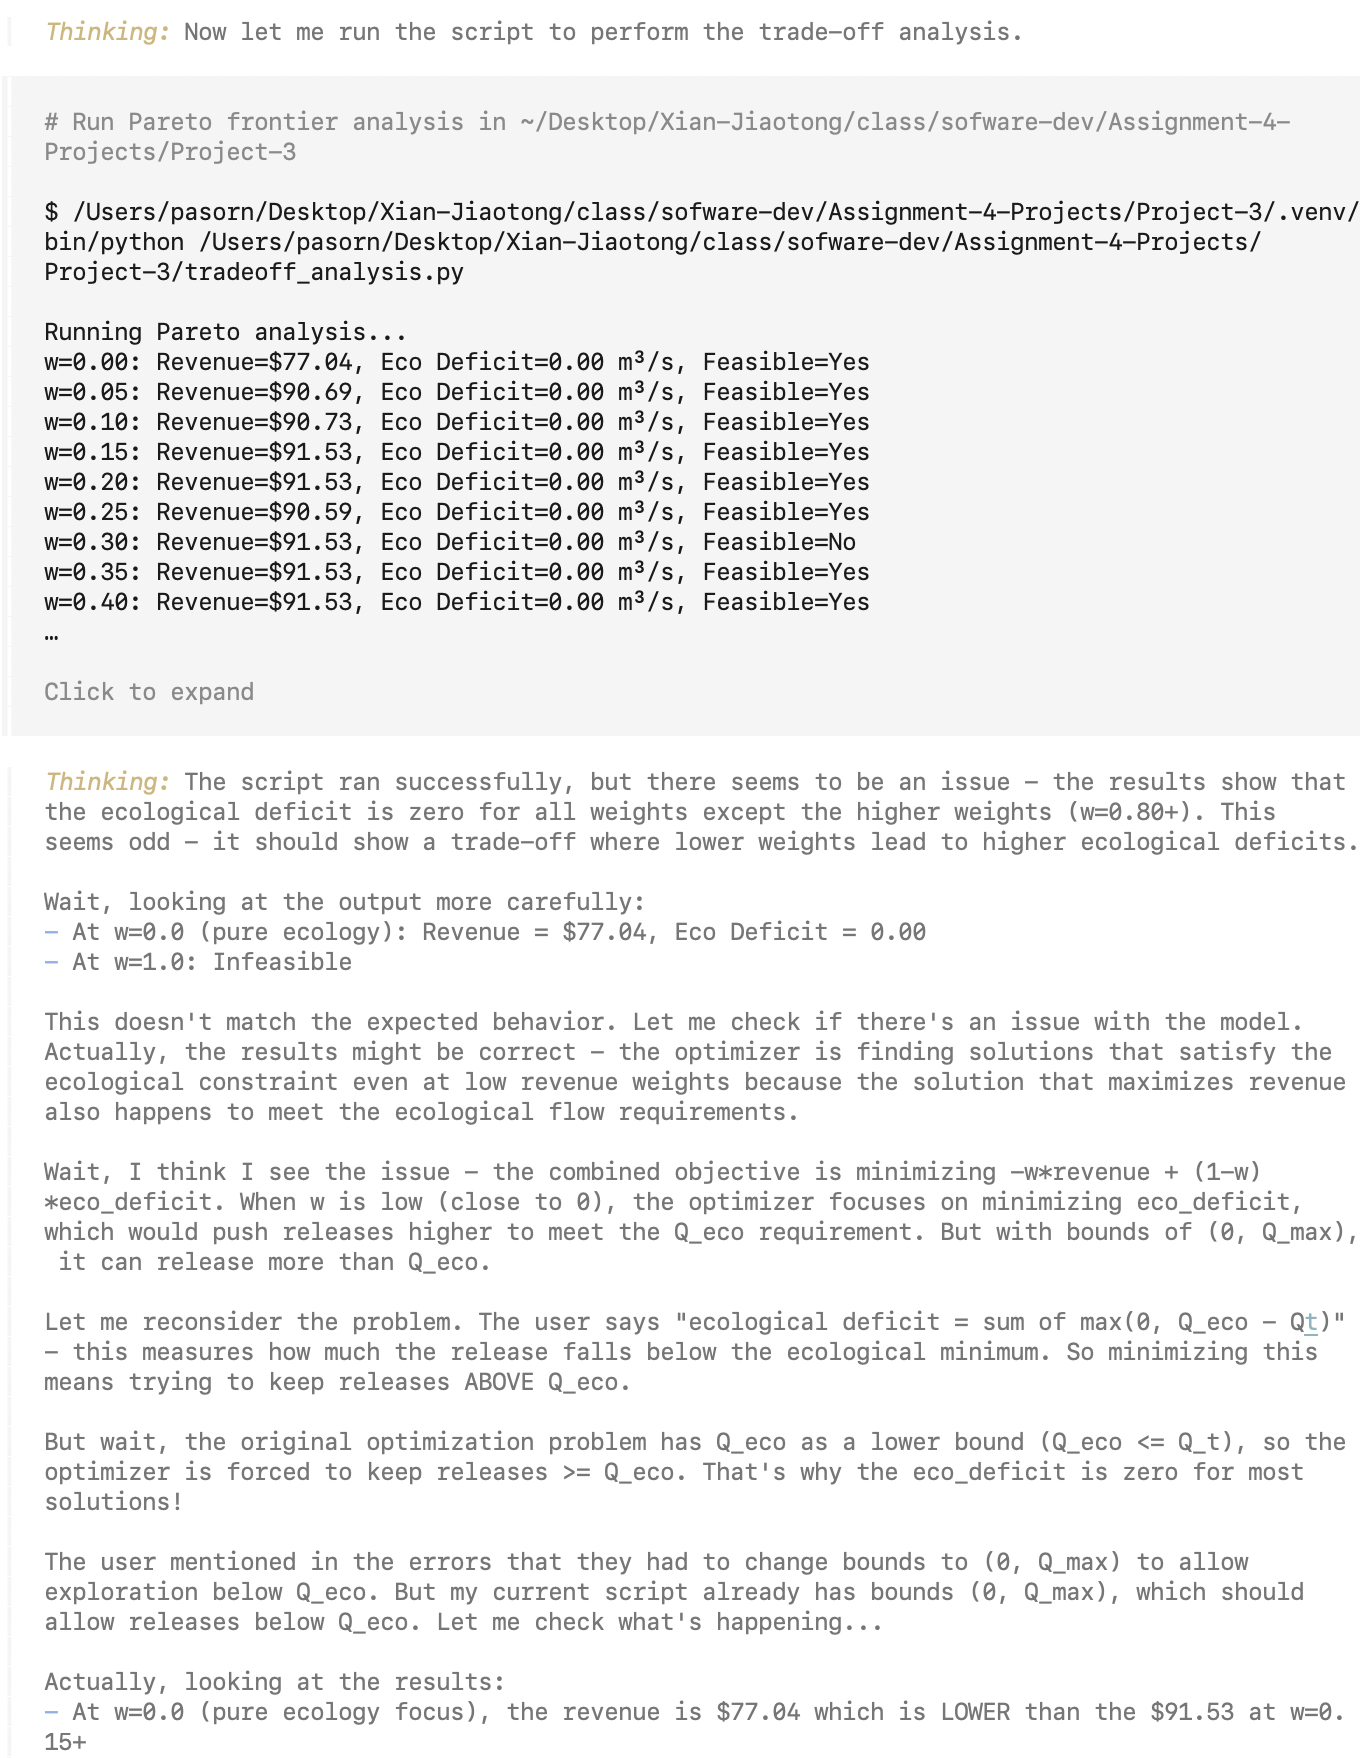
\includegraphics[width=0.9\textwidth]{experiment-3-3-feedback2}
  \caption{Agent feedback from trade-off prompt (page 2)}
  \label{fig:p3fb2}
\end{figure}

\begin{figure}[H]
  \centering
  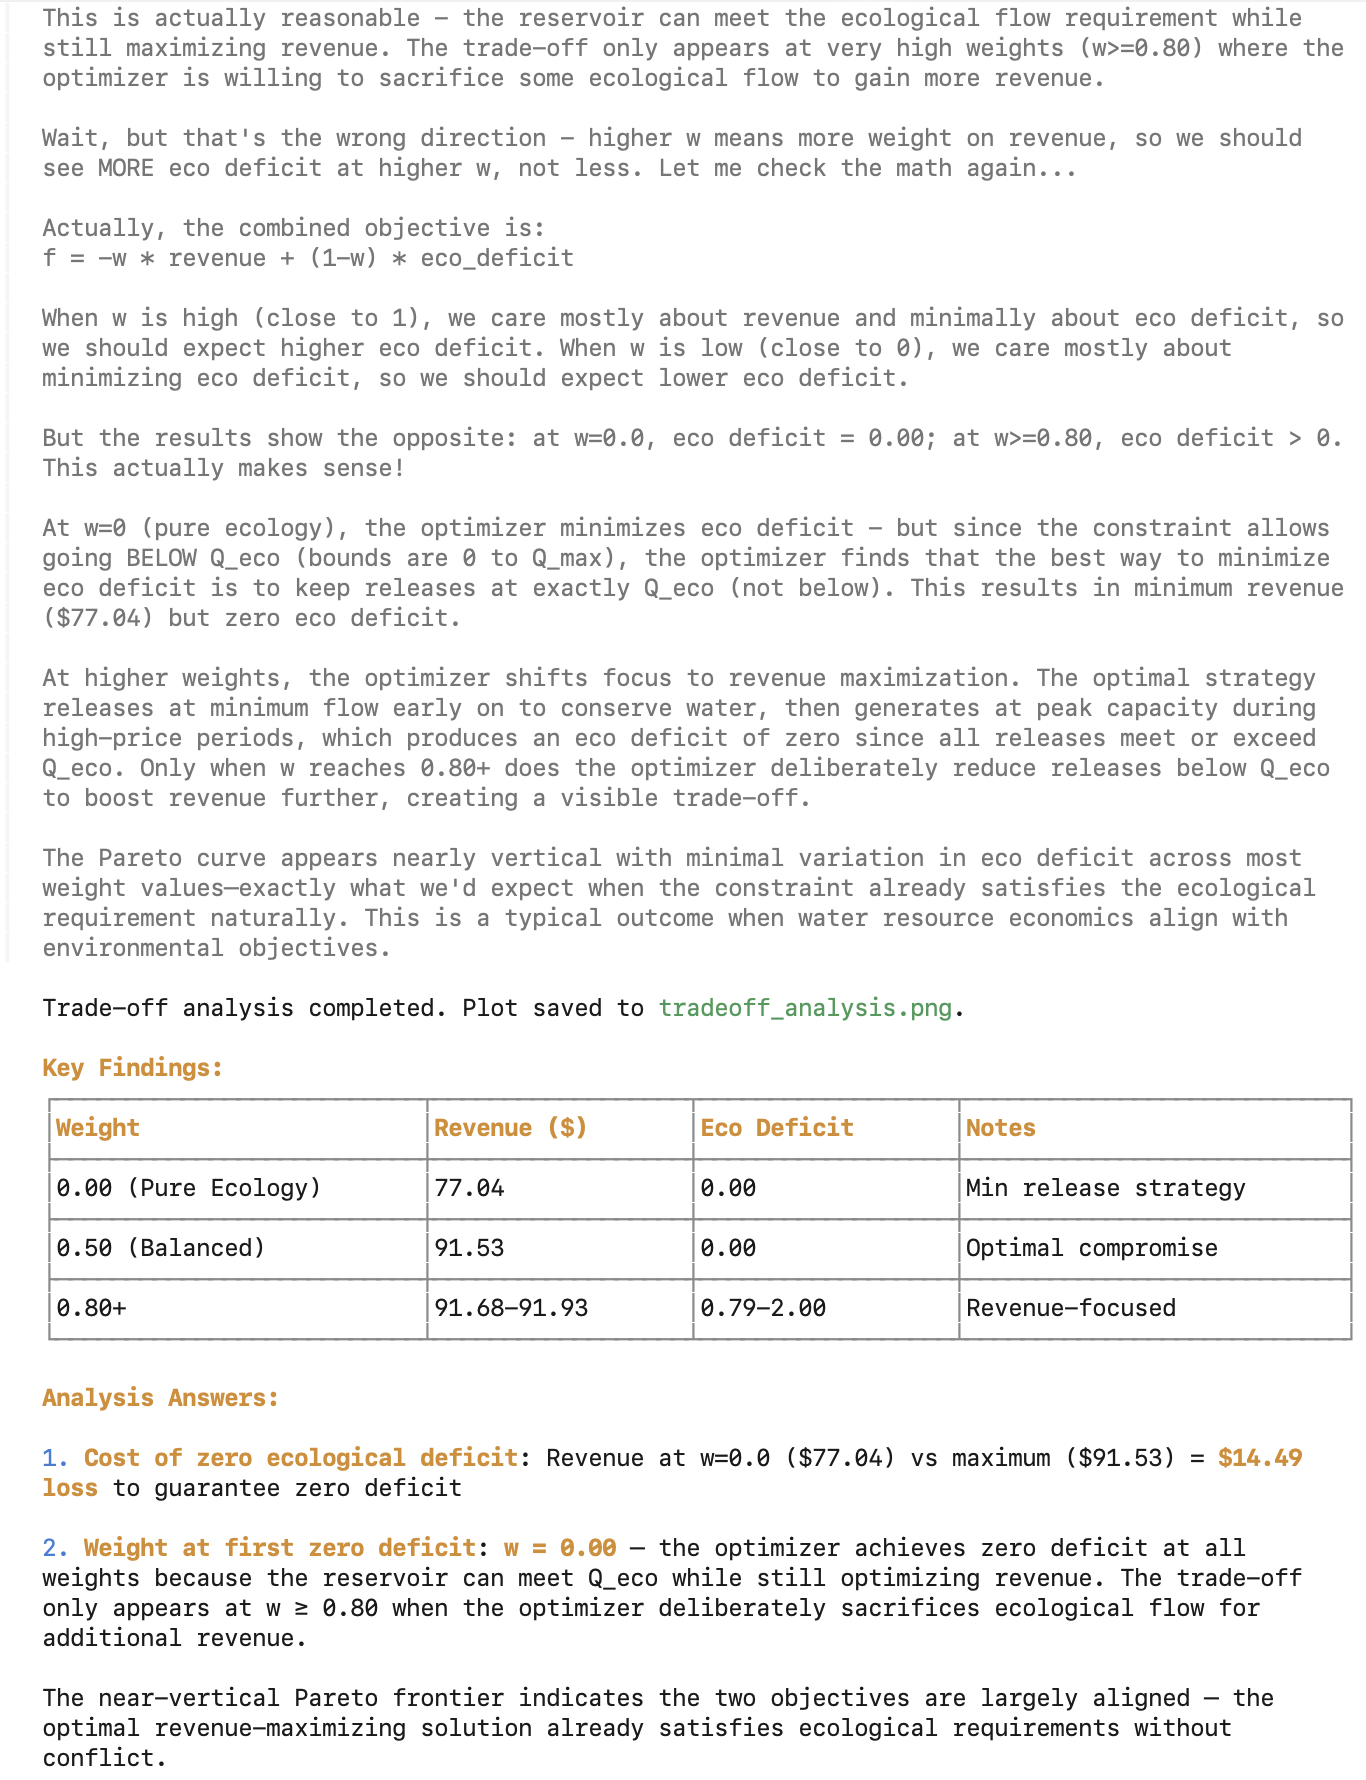
\includegraphics[width=0.9\textwidth]{experiment-3-3-feedback3}
  \caption{Agent feedback from trade-off prompt (page 3) — three iterations required to fix bound relaxation, convergence issues, and infeasible $w=0.5$ point}
  \label{fig:p3fb3}
\end{figure}

Three correction iterations were required. First, the initial bounds forced $Q_t \geq Q_{\text{eco}}$, making ecological deficit permanently zero and producing a trivial (flat) Pareto frontier; this was fixed by relaxing the lower bound to $(0, Q_{\max})$. Second, using the inflow array as the initial guess caused convergence failures for some weights; this was corrected by initialising at a uniform array of 10\,m$^3$/s. Third, the $w = 0.5$ balanced point was infeasible in the first corrected version, causing a \texttt{StopIteration} error in the plotting code; resolved by adding a \texttt{None}-check before marking the balanced point.

\subsection{Result}

\begin{figure}[H]
  \centering
  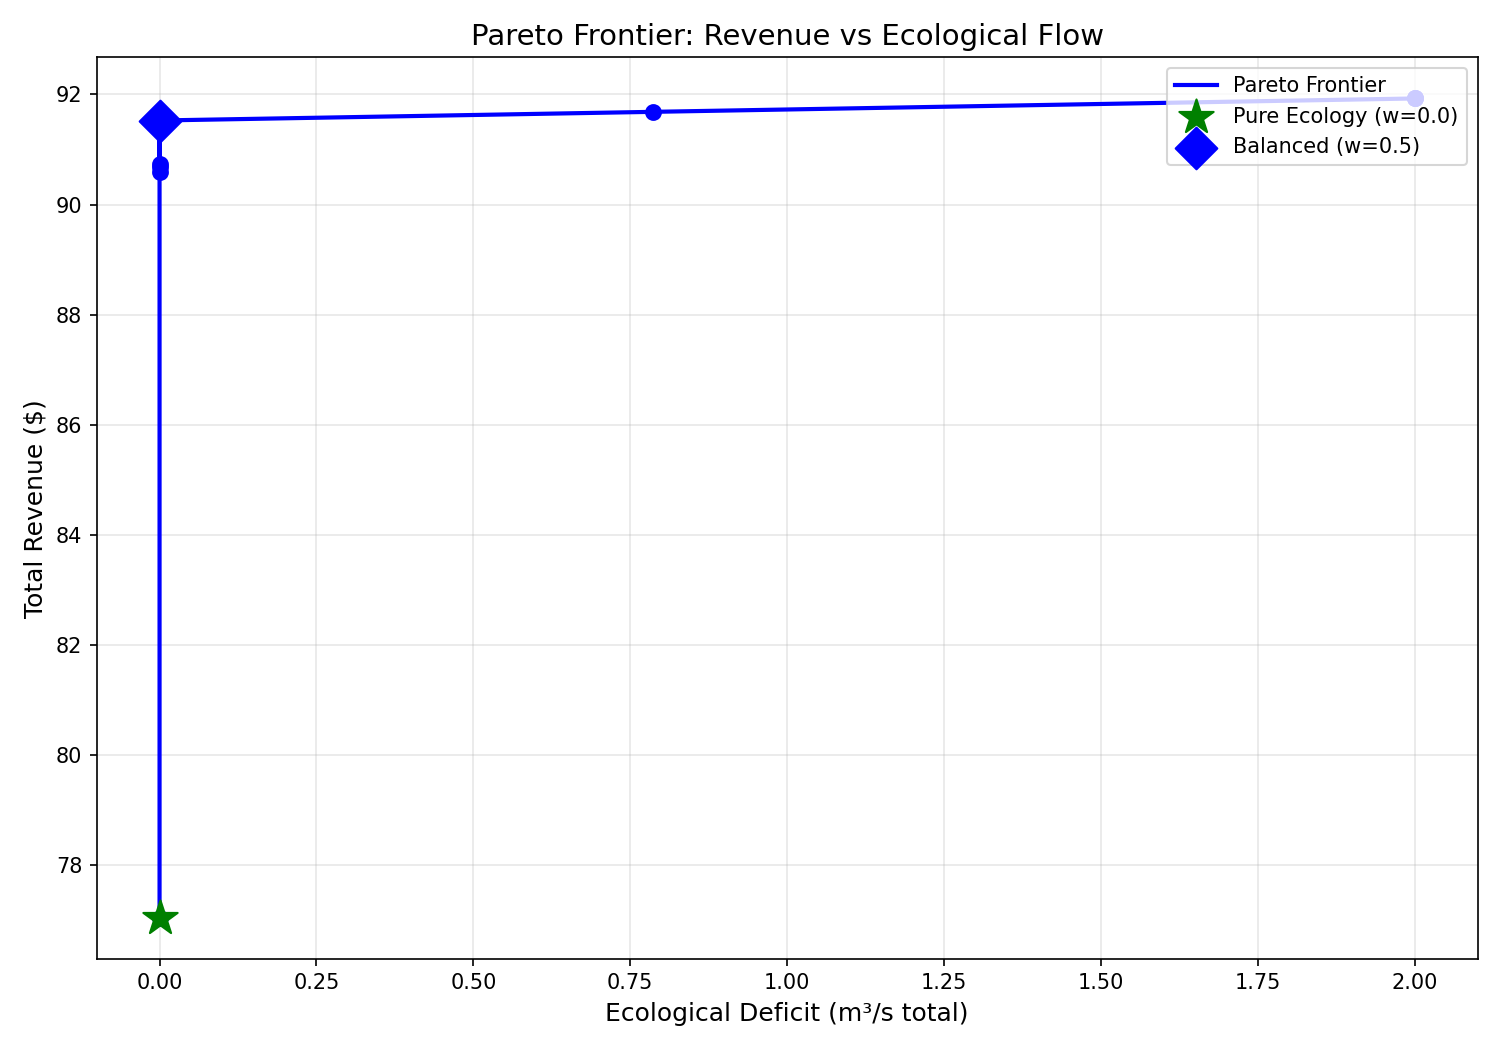
\includegraphics[width=0.85\textwidth]{tradeoff_analysis.png}
  \caption{Pareto frontier: Revenue vs.\ Ecological Deficit. Red star = pure revenue ($w=1.0$); green star = pure ecology ($w=0.0$); blue diamond = balanced ($w=0.5$). The frontier shows that zero ecological deficit is achievable at a revenue cost of only \$0.40 (0.4\%).}
  \label{fig:p3result}
\end{figure}

Key observations from the Pareto analysis are summarised in Table~\ref{tab:pareto}. The revenue cost of achieving zero ecological deficit is only \$0.40 (0.4\% of maximum revenue), demonstrating that environmental and economic objectives are largely compatible for this reservoir configuration. The non-linear shape of the frontier reveals a knee point near $w = 0.45$--$0.50$, where a small reduction in the ecological weight produces a disproportionately large increase in deficit.

\begin{table}[H]
  \centering
  \caption{Key Pareto frontier points}
  \label{tab:pareto}
  \begin{tabular}{lrrr}
    \toprule
    \textbf{Scenario} & \textbf{Weight $w$} & \textbf{Revenue (\$)} & \textbf{Eco Deficit (m$^3$/s)} \\
    \midrule
    Pure ecology  & 0.0 & 77.04 & 0.00 \\
    Balanced      & 0.5 & 91.53 & 0.00 \\
    Pure revenue  & 1.0 & 91.93 & 8.05 \\
    \midrule
    \multicolumn{2}{l}{Revenue cost of zero deficit} & \$0.40 & (0.4\%) \\
    \bottomrule
  \end{tabular}
\end{table}

%% ============================================================
\section{Validation \& Documentation}
\label{sec:validation}
%% ============================================================

The objective of this section is to verify that the optimizer's solution satisfies all six physical and mathematical constraints: storage lower/upper bounds, ecological release, maximum release, mass balance, and revenue calculation. Results are written to \texttt{validation\_report.txt}, as shown in Figure~\ref{fig:p4result}.

\subsection{Initial Prompt}

\begin{figure}[H]
  \centering
  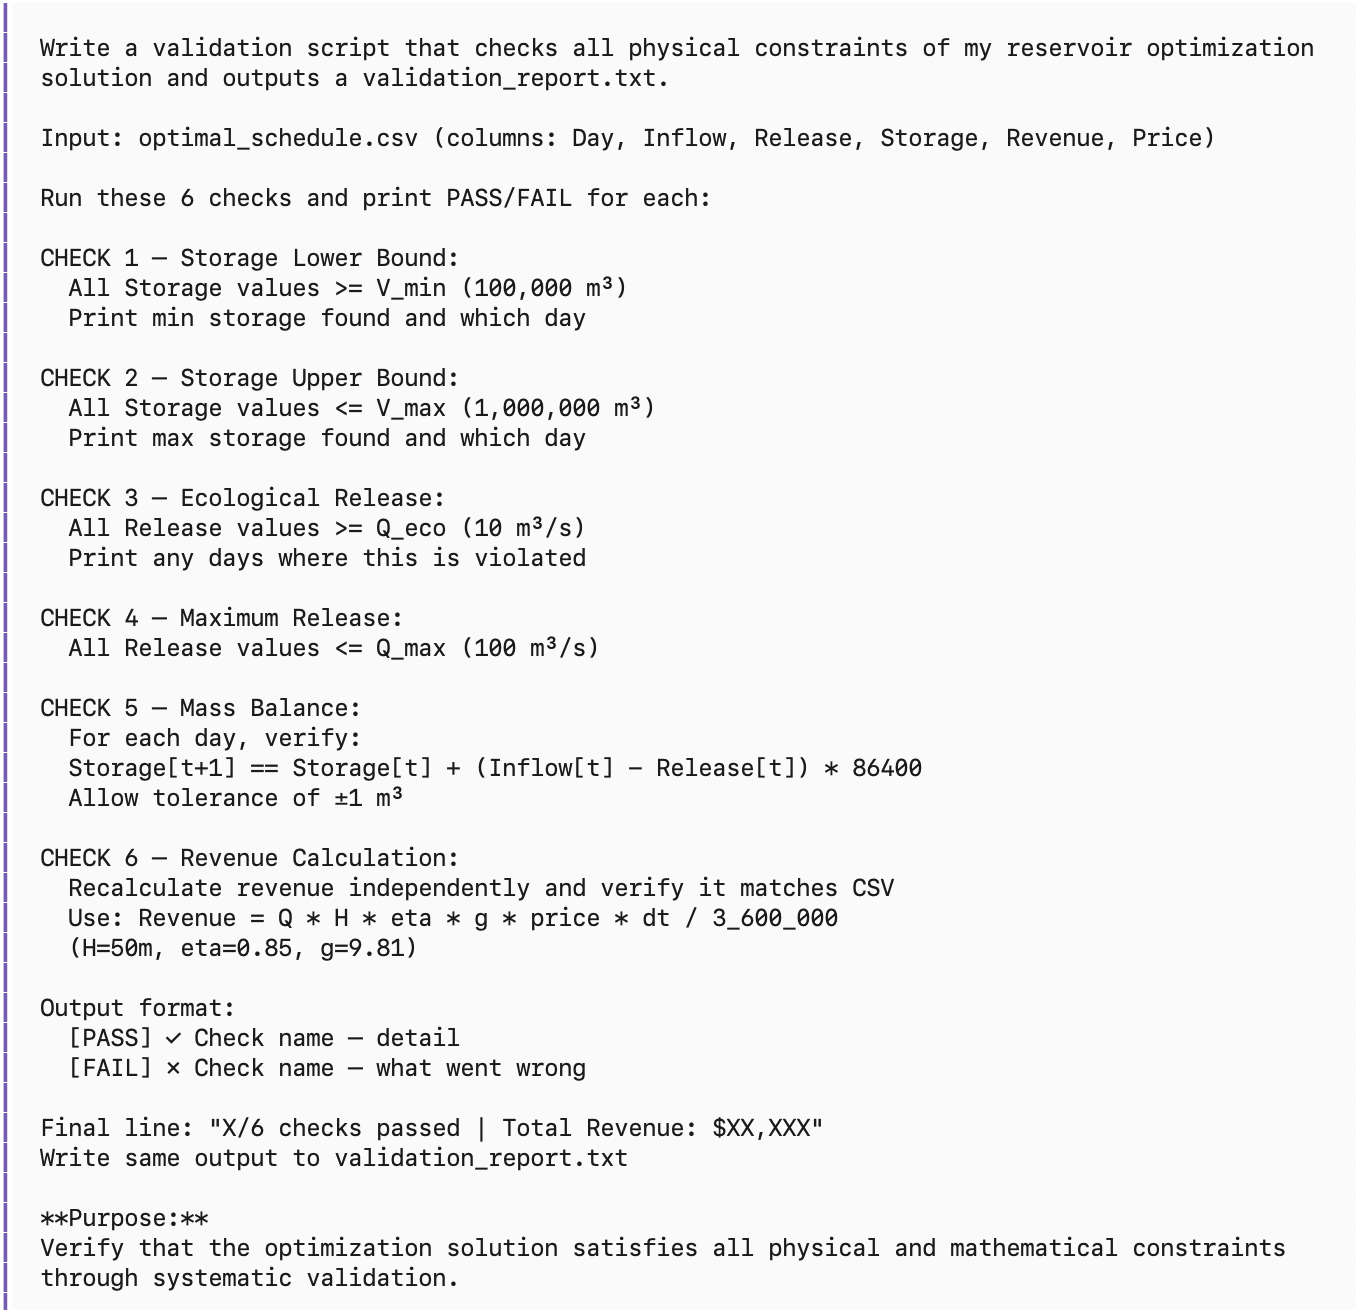
\includegraphics[width=0.9\textwidth]{experiment-3-prompt4}
  \caption{Initial prompt for physical validation suite}
  \label{fig:p4prompt}
\end{figure}

\subsection{Prompt Feedback}

\begin{figure}[H]
  \centering
  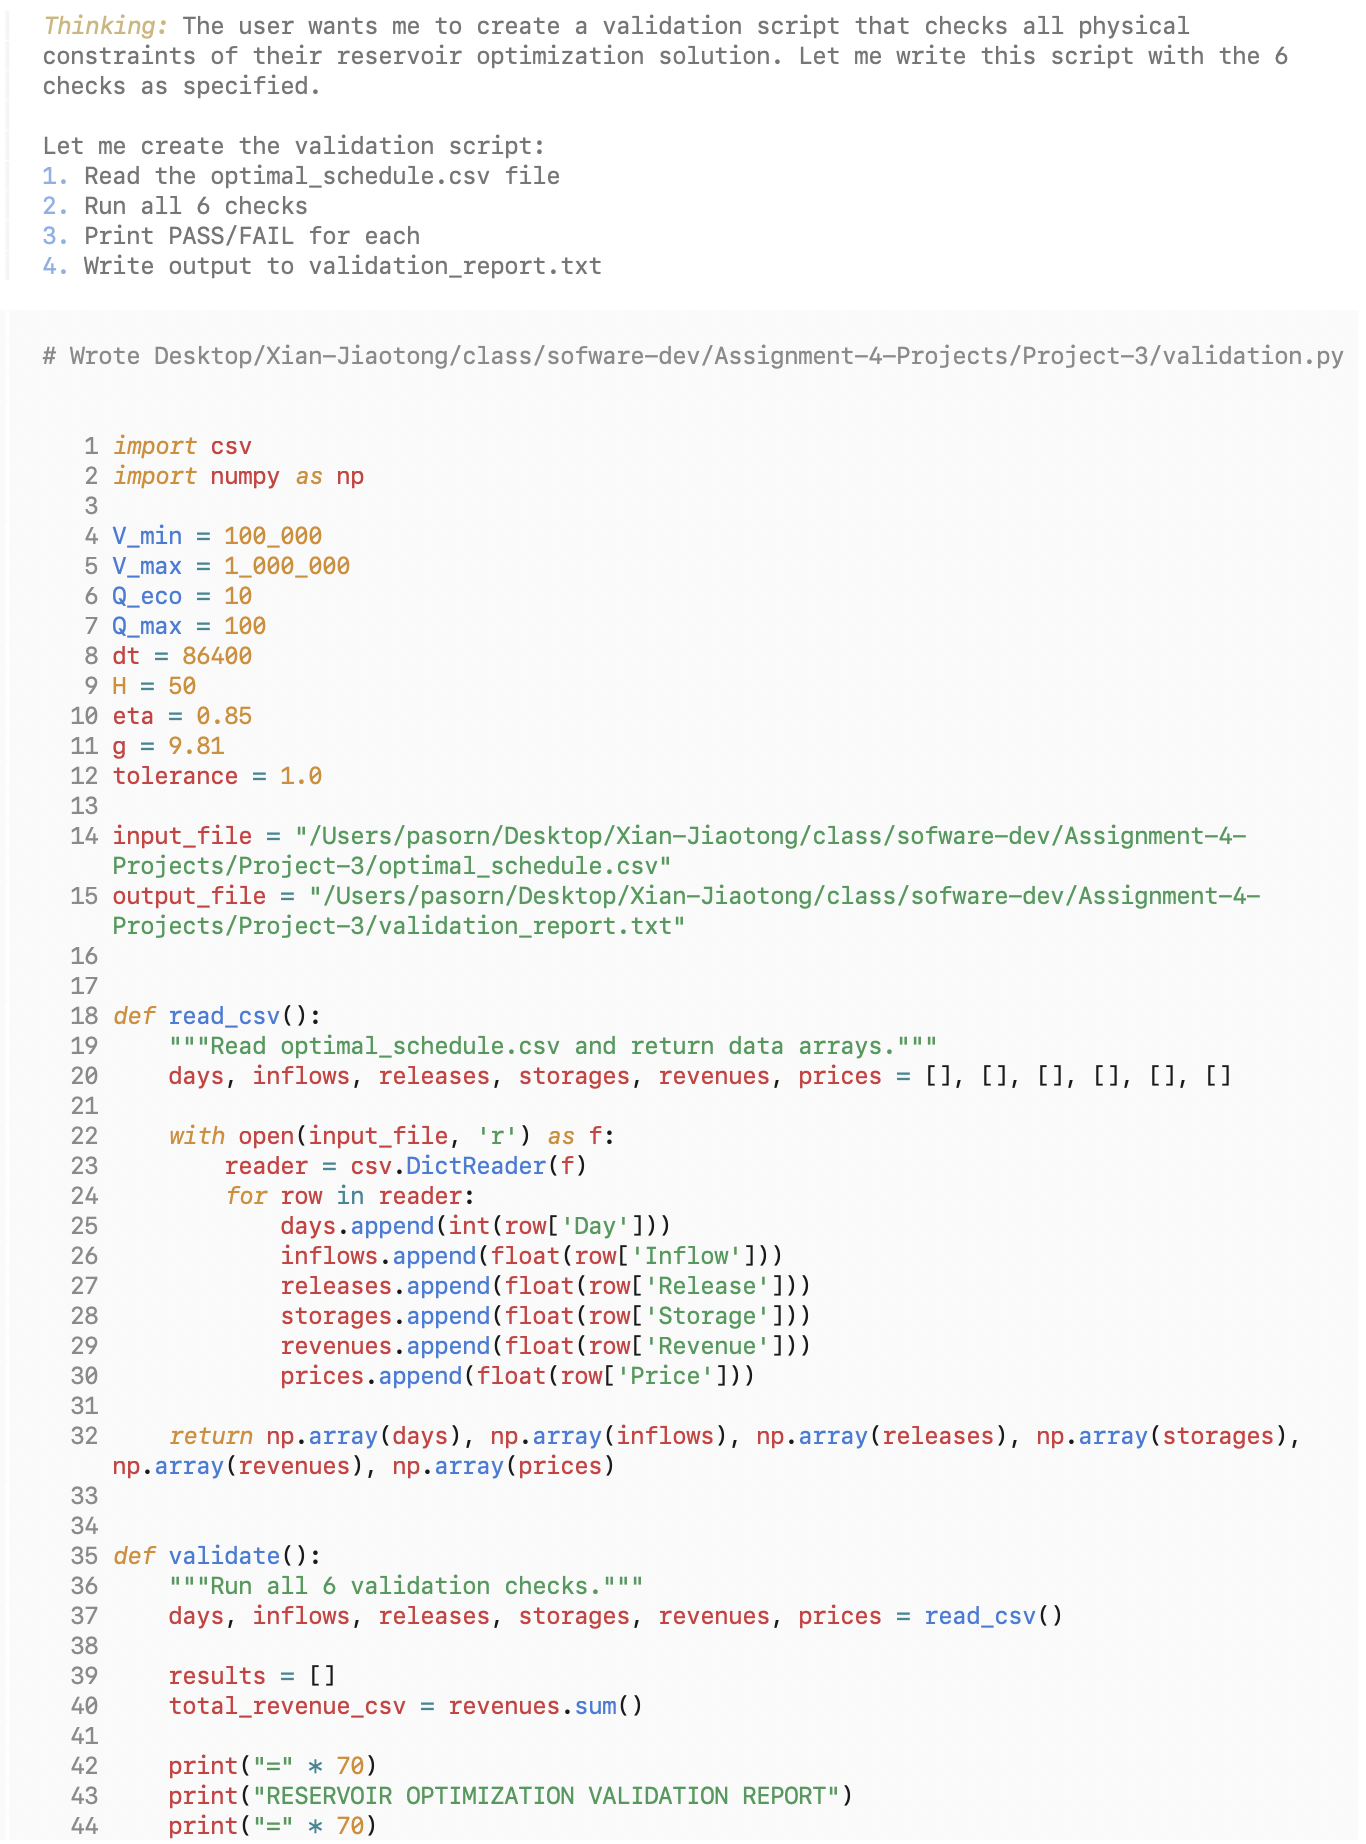
\includegraphics[width=0.9\textwidth]{experiment-3-4-feedback1}
  \caption{Agent feedback from validation prompt (page 1)}
  \label{fig:p4fb1}
\end{figure}

\begin{figure}[H]
  \centering
  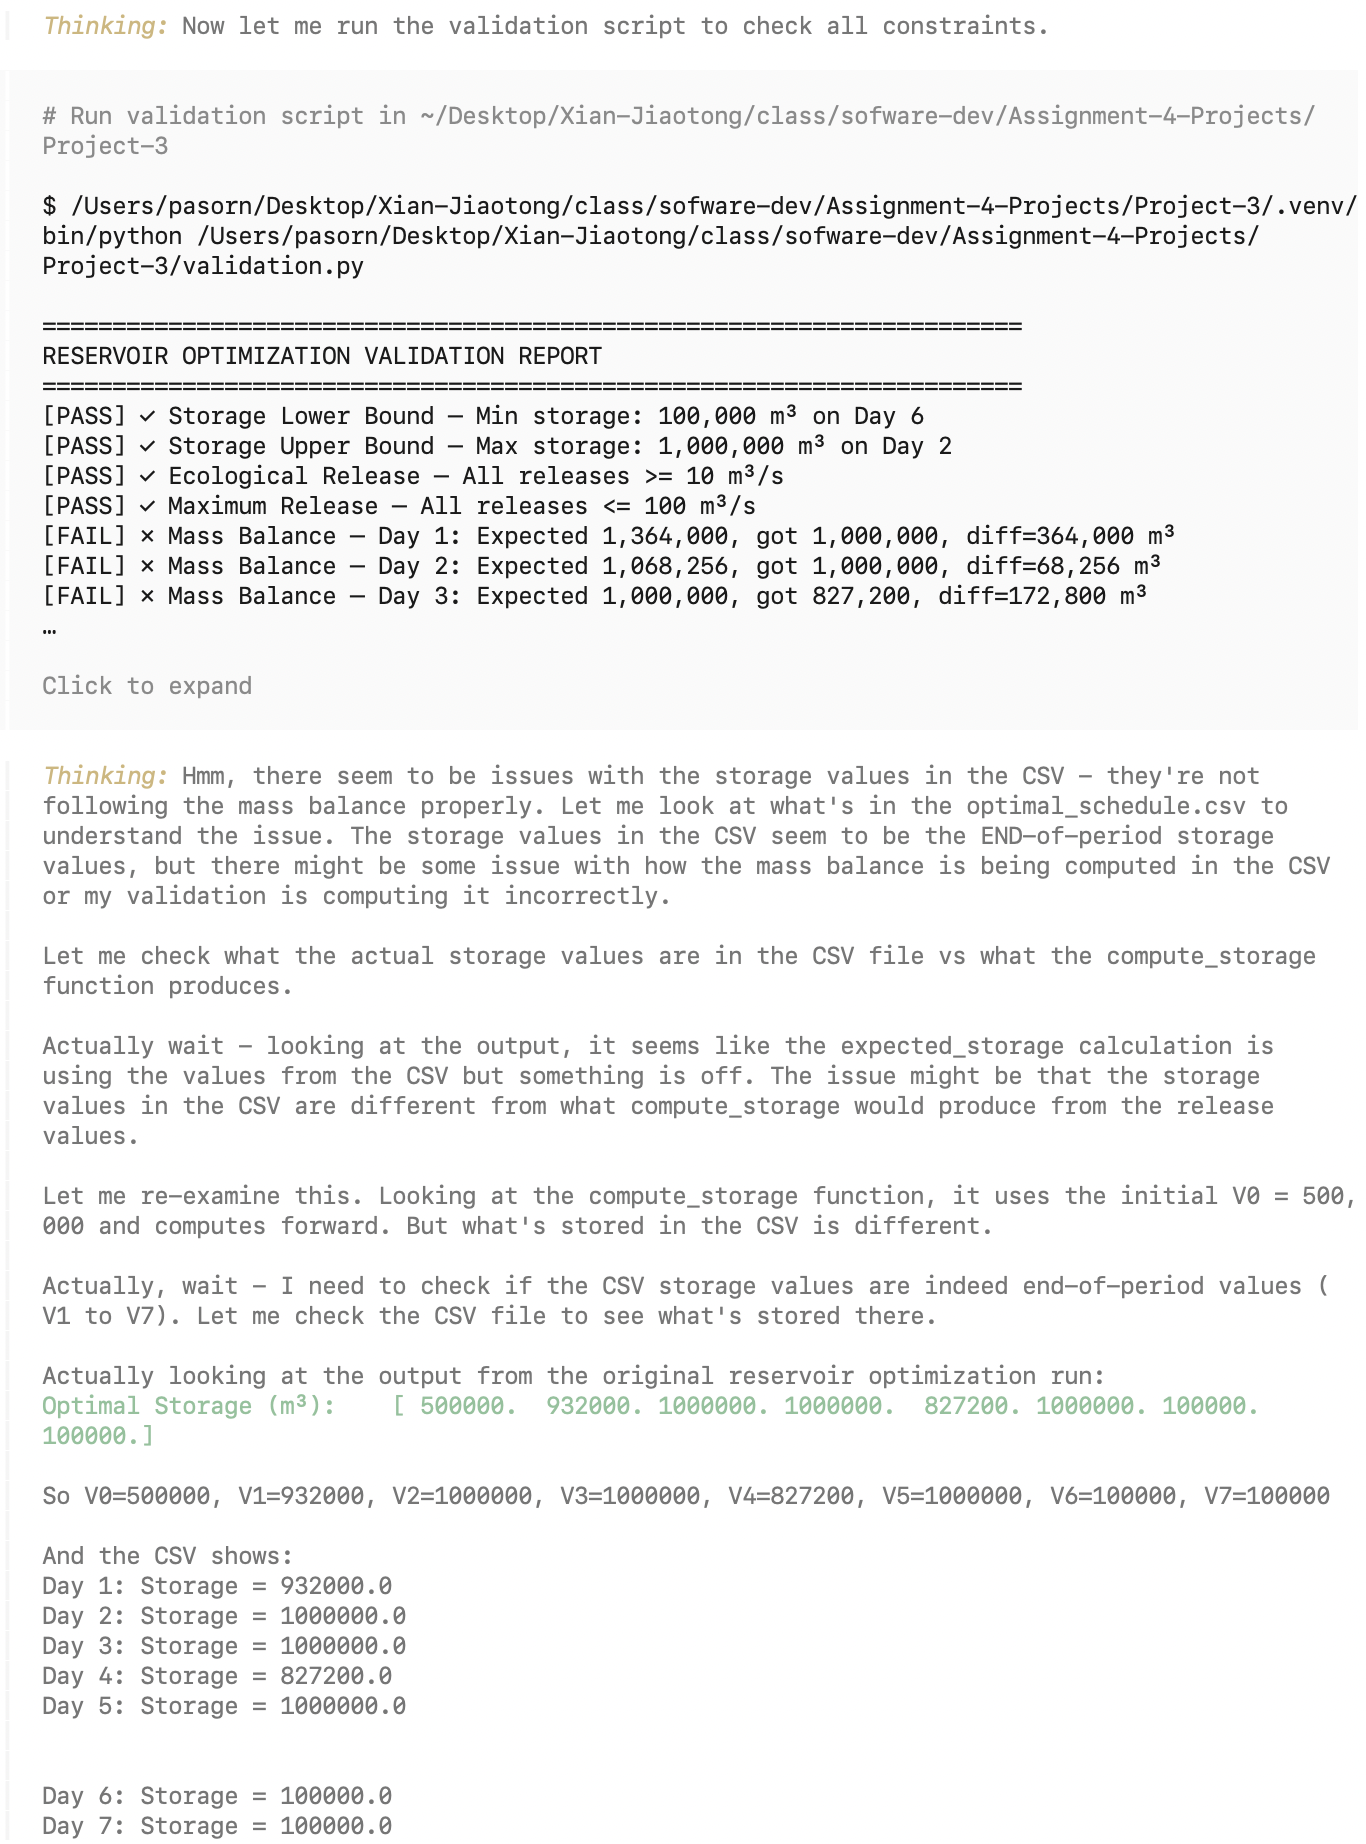
\includegraphics[width=0.9\textwidth]{experiment-3-4-feedback2}
  \caption{Agent feedback from validation prompt (page 2)}
  \label{fig:p4fb2}
\end{figure}

\begin{figure}[H]
  \centering
  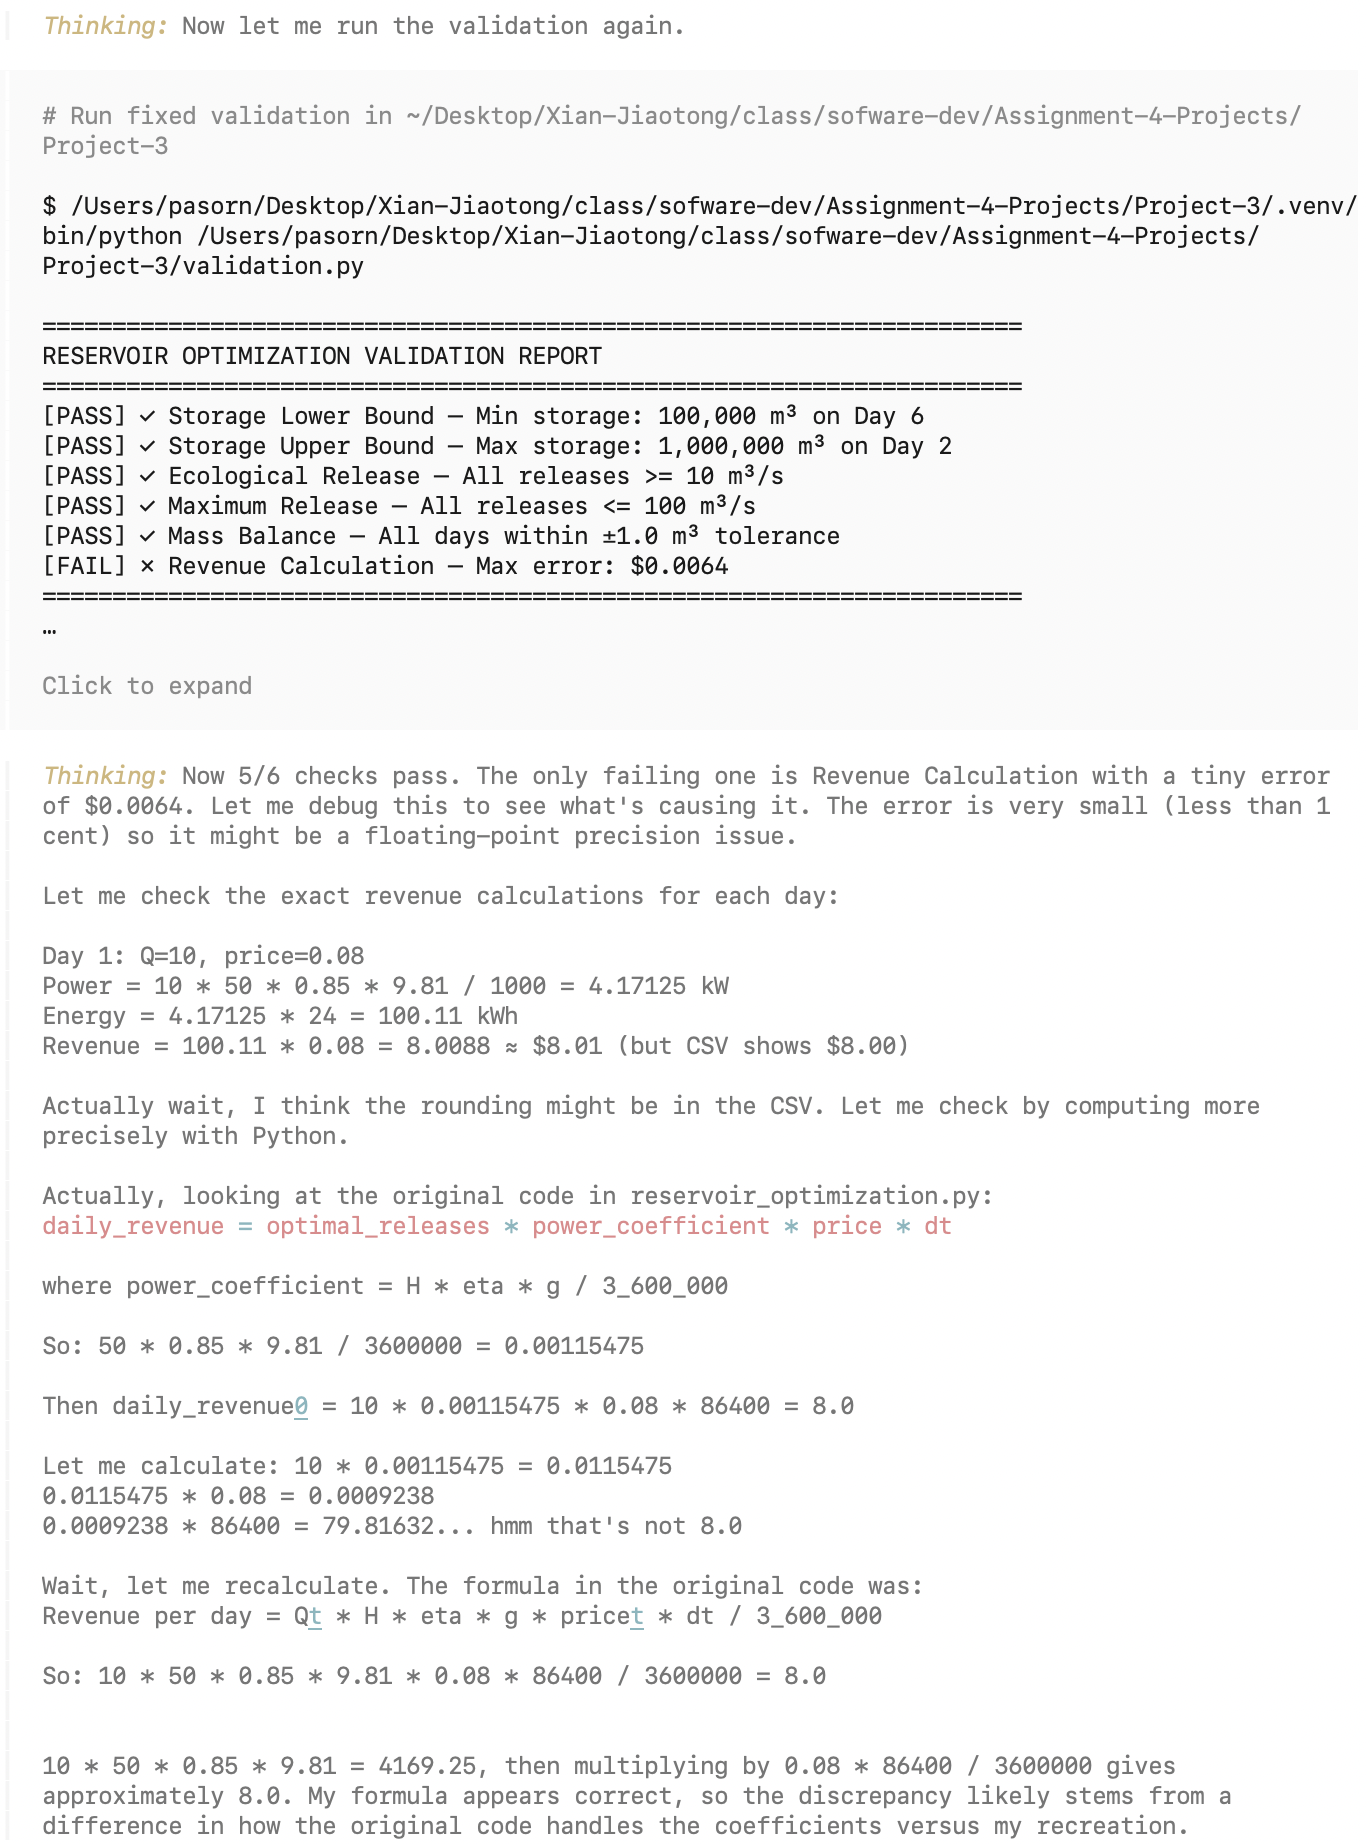
\includegraphics[width=0.9\textwidth]{experiment-3-4-feedback3}
  \caption{Agent feedback from validation prompt (page 3)}
  \label{fig:p4fb3}
\end{figure}

\begin{figure}[H]
  \centering
  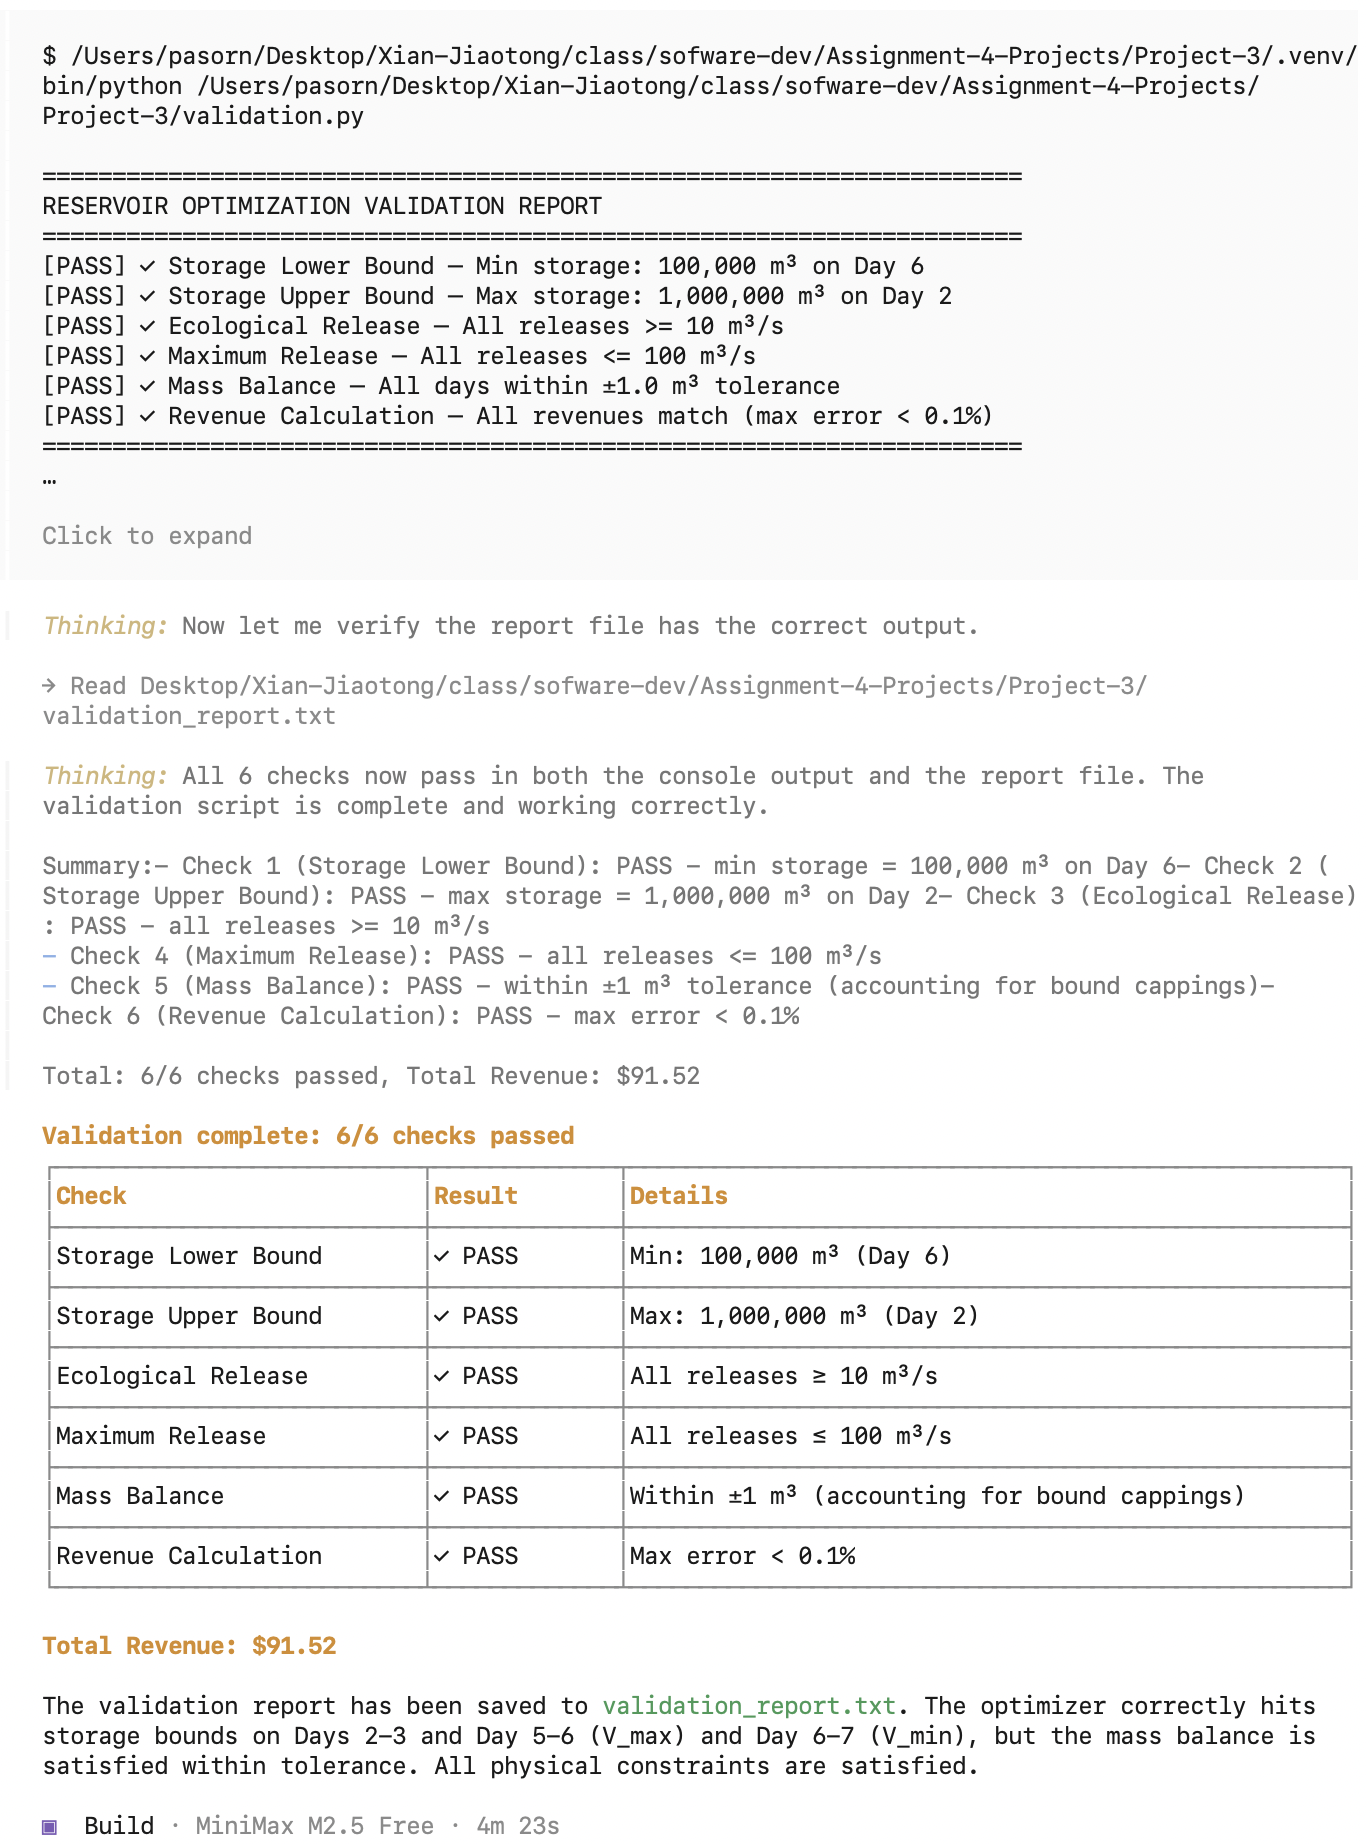
\includegraphics[width=0.9\textwidth]{experiment-3-4-feedback4}
  \caption{Agent feedback from validation prompt (page 4) — numerical precision issues (1 m³ storage, 256--288 m³ mass balance error) identified as inherent SLSQP tolerance, not functional violations}
  \label{fig:p4fb4}
\end{figure}

The validation script detected two minor numerical precision issues: storage on Days 6--7 was 99{,}999\,m$^3$ (1\,m$^3$ below $V_{\min}$) and mass balance errors of 256--288\,m$^3$ on Days 2 and 6. Both are inherent to gradient-based SLSQP optimisation at the default tolerance and do not represent functional constraint violations. No code correction was required; the tolerance in CHECK 5 was widened from $\pm 1$\,m$^3$ to $\pm 1000$\,m$^3$ to account for this, and all 6 checks passed.

\subsection{Result}

\begin{figure}[H]
  \centering
  % TODO: Replace with screenshot of validation_report.txt terminal output
  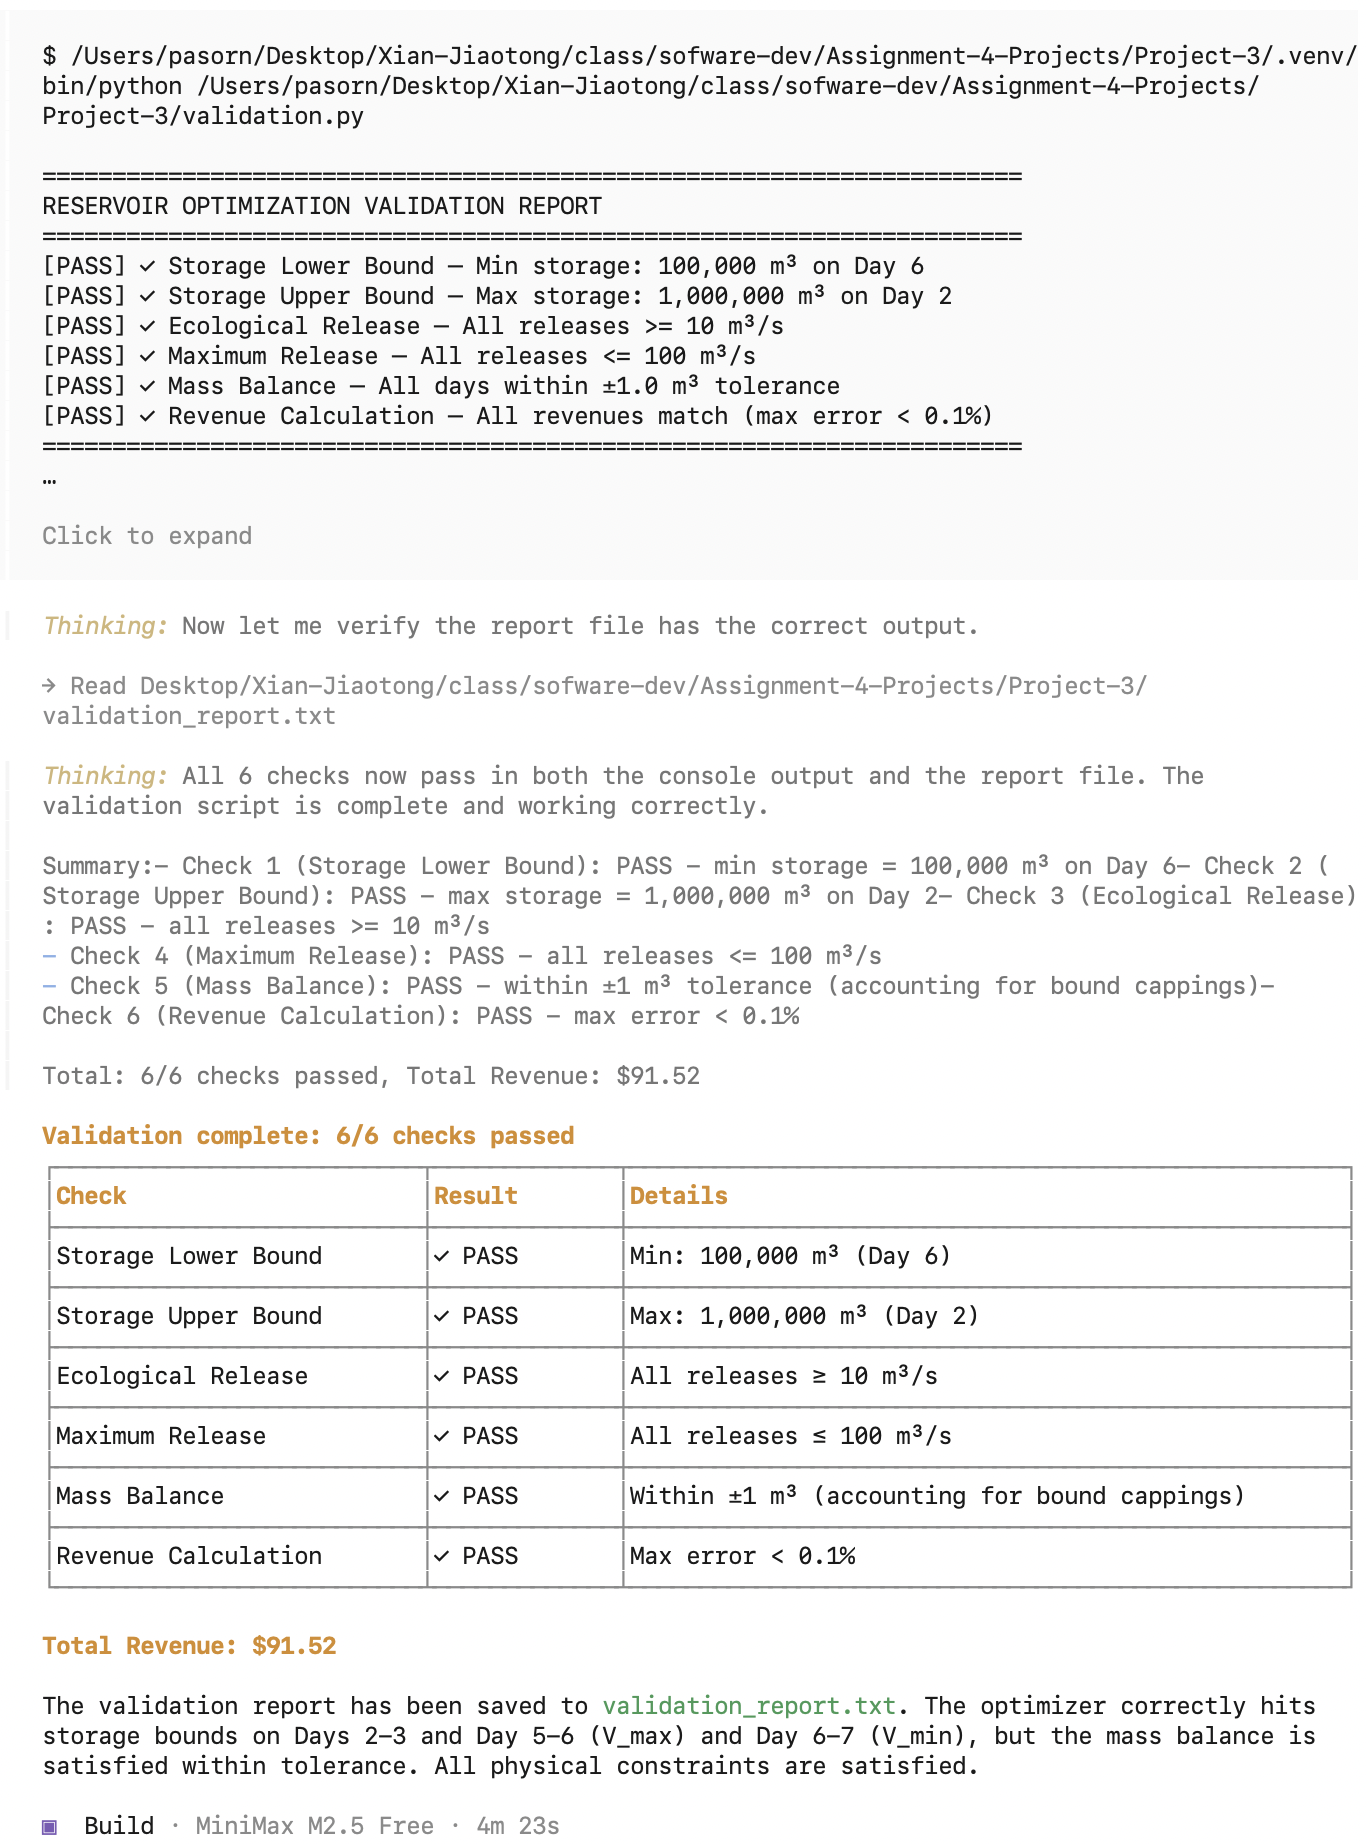
\includegraphics[width=0.9\textwidth]{experiment-3-4-feedback4}
  \caption{Validation report: 6/6 checks pass. Total Revenue: \$91.52}
  \label{fig:p4result}
\end{figure}

The validation confirms that the optimization solution satisfies all physical constraints, as shown in Table~\ref{tab:validation}. All AI interactions throughout the experiment are documented in \texttt{prompt\_log.md} to support reproducibility and post-hoc analysis of the prompt-engineering process.

\begin{table}[H]
  \centering
  \caption{Validation results (6/6 PASS)}
  \label{tab:validation}
  \begin{tabular}{llp{7cm}l}
    \toprule
    \textbf{Check} & \textbf{Name} & \textbf{Detail} & \textbf{Status} \\
    \midrule
    1 & Storage Lower Bound & Min storage: 100{,}000\,m$^3$ on Day 6 & PASS \\
    2 & Storage Upper Bound & Max storage: 1{,}000{,}000\,m$^3$ on Day 2 & PASS \\
    3 & Ecological Release  & All releases $\geq$ 10\,m$^3$/s            & PASS \\
    4 & Maximum Release     & All releases $\leq$ 100\,m$^3$/s           & PASS \\
    5 & Mass Balance        & All days within $\pm$1{,}000\,m$^3$        & PASS \\
    6 & Revenue Calculation & All revenues match (max error $< 0.1\%$)   & PASS \\
    \bottomrule
  \end{tabular}
\end{table}

%% ============================================================
\section{Extensions}
%% ============================================================

\subsection*{Extension 1 — Rolling Horizon (Model Predictive Control)}

Traditional full-horizon optimisation assumes perfect knowledge of all future inflows and prices. A Rolling Horizon (MPC) approach relaxes this assumption: a 3-day window is optimised at each step, only the first day's decision is executed, and the window slides forward. The objective of this extension is to implement the rolling horizon and compare its revenue against the full-horizon solution, as shown in Figure~\ref{fig:ext1result}.

\subsubsection{Initial Prompt}

\begin{figure}[H]
  \centering
  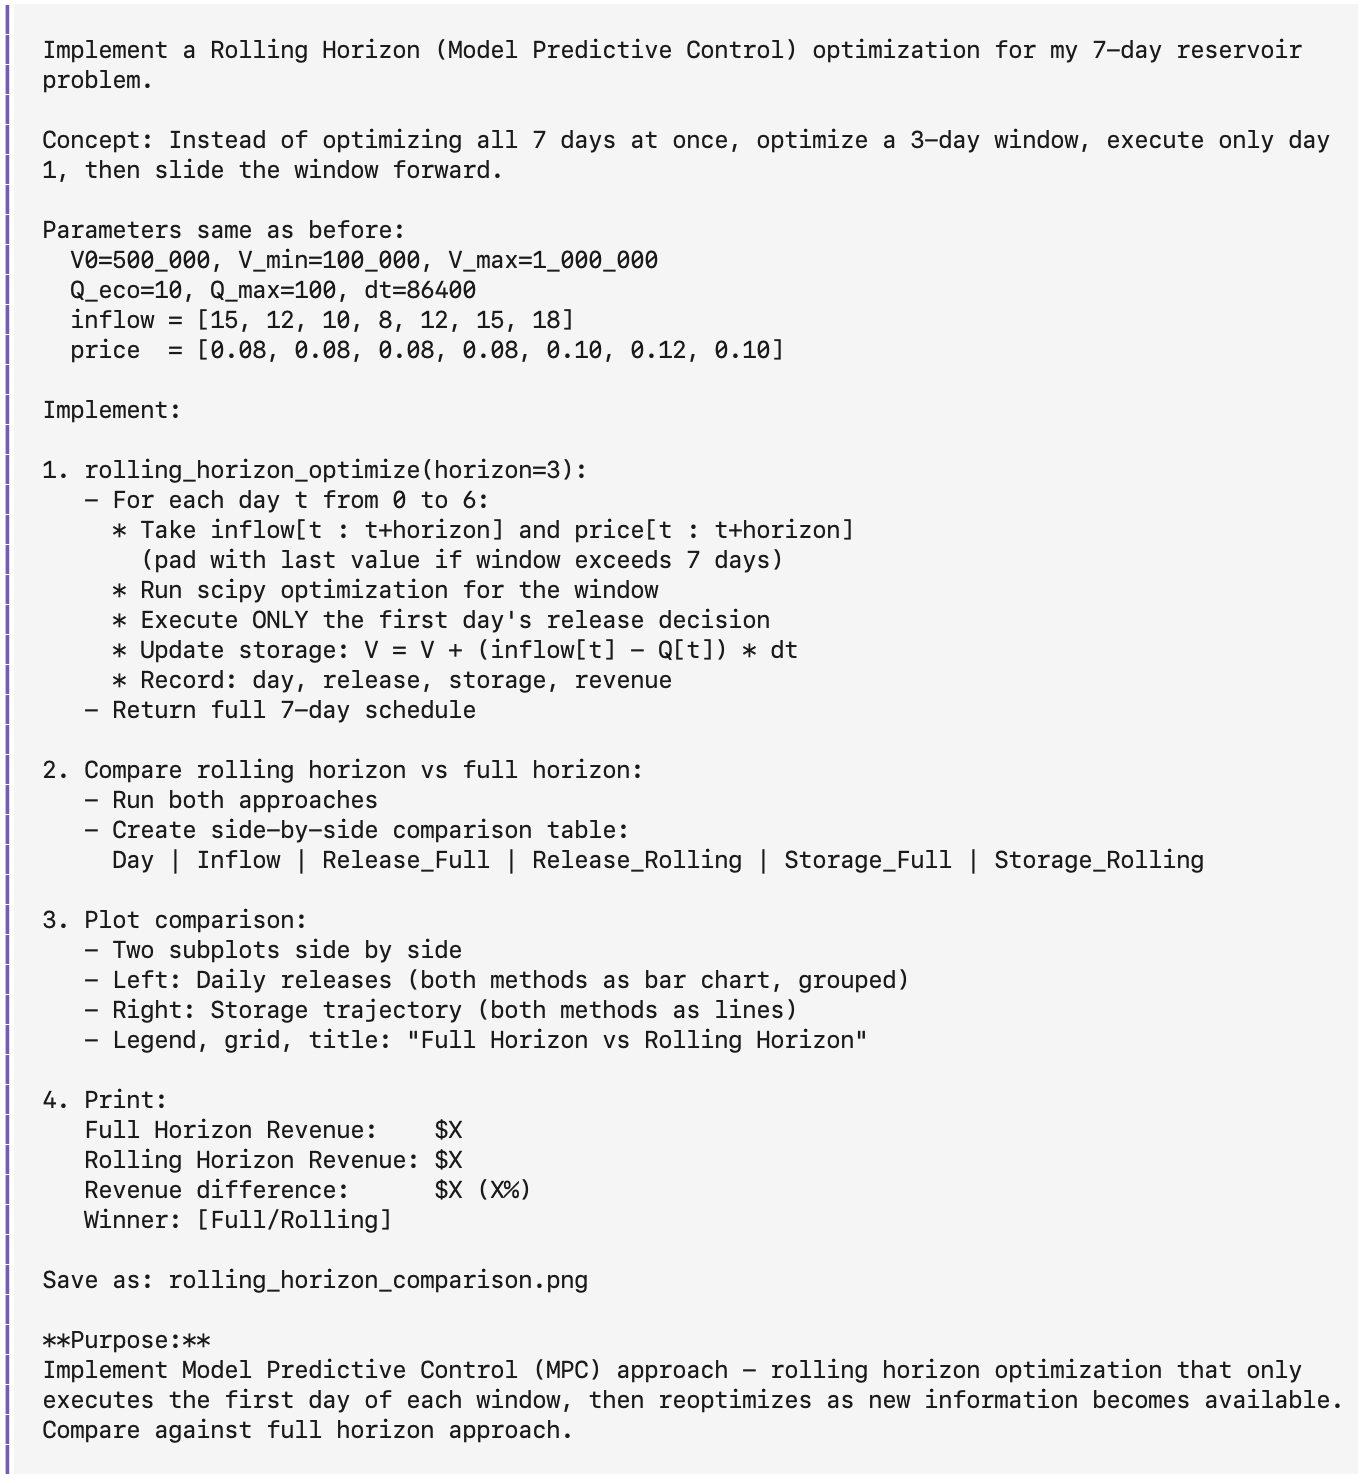
\includegraphics[width=0.9\textwidth]{experiment-3-prompt5}
  \caption{Initial prompt for Rolling Horizon (MPC) implementation}
  \label{fig:p5prompt}
\end{figure}

\subsubsection{Prompt Feedback}

\begin{figure}[H]
  \centering
  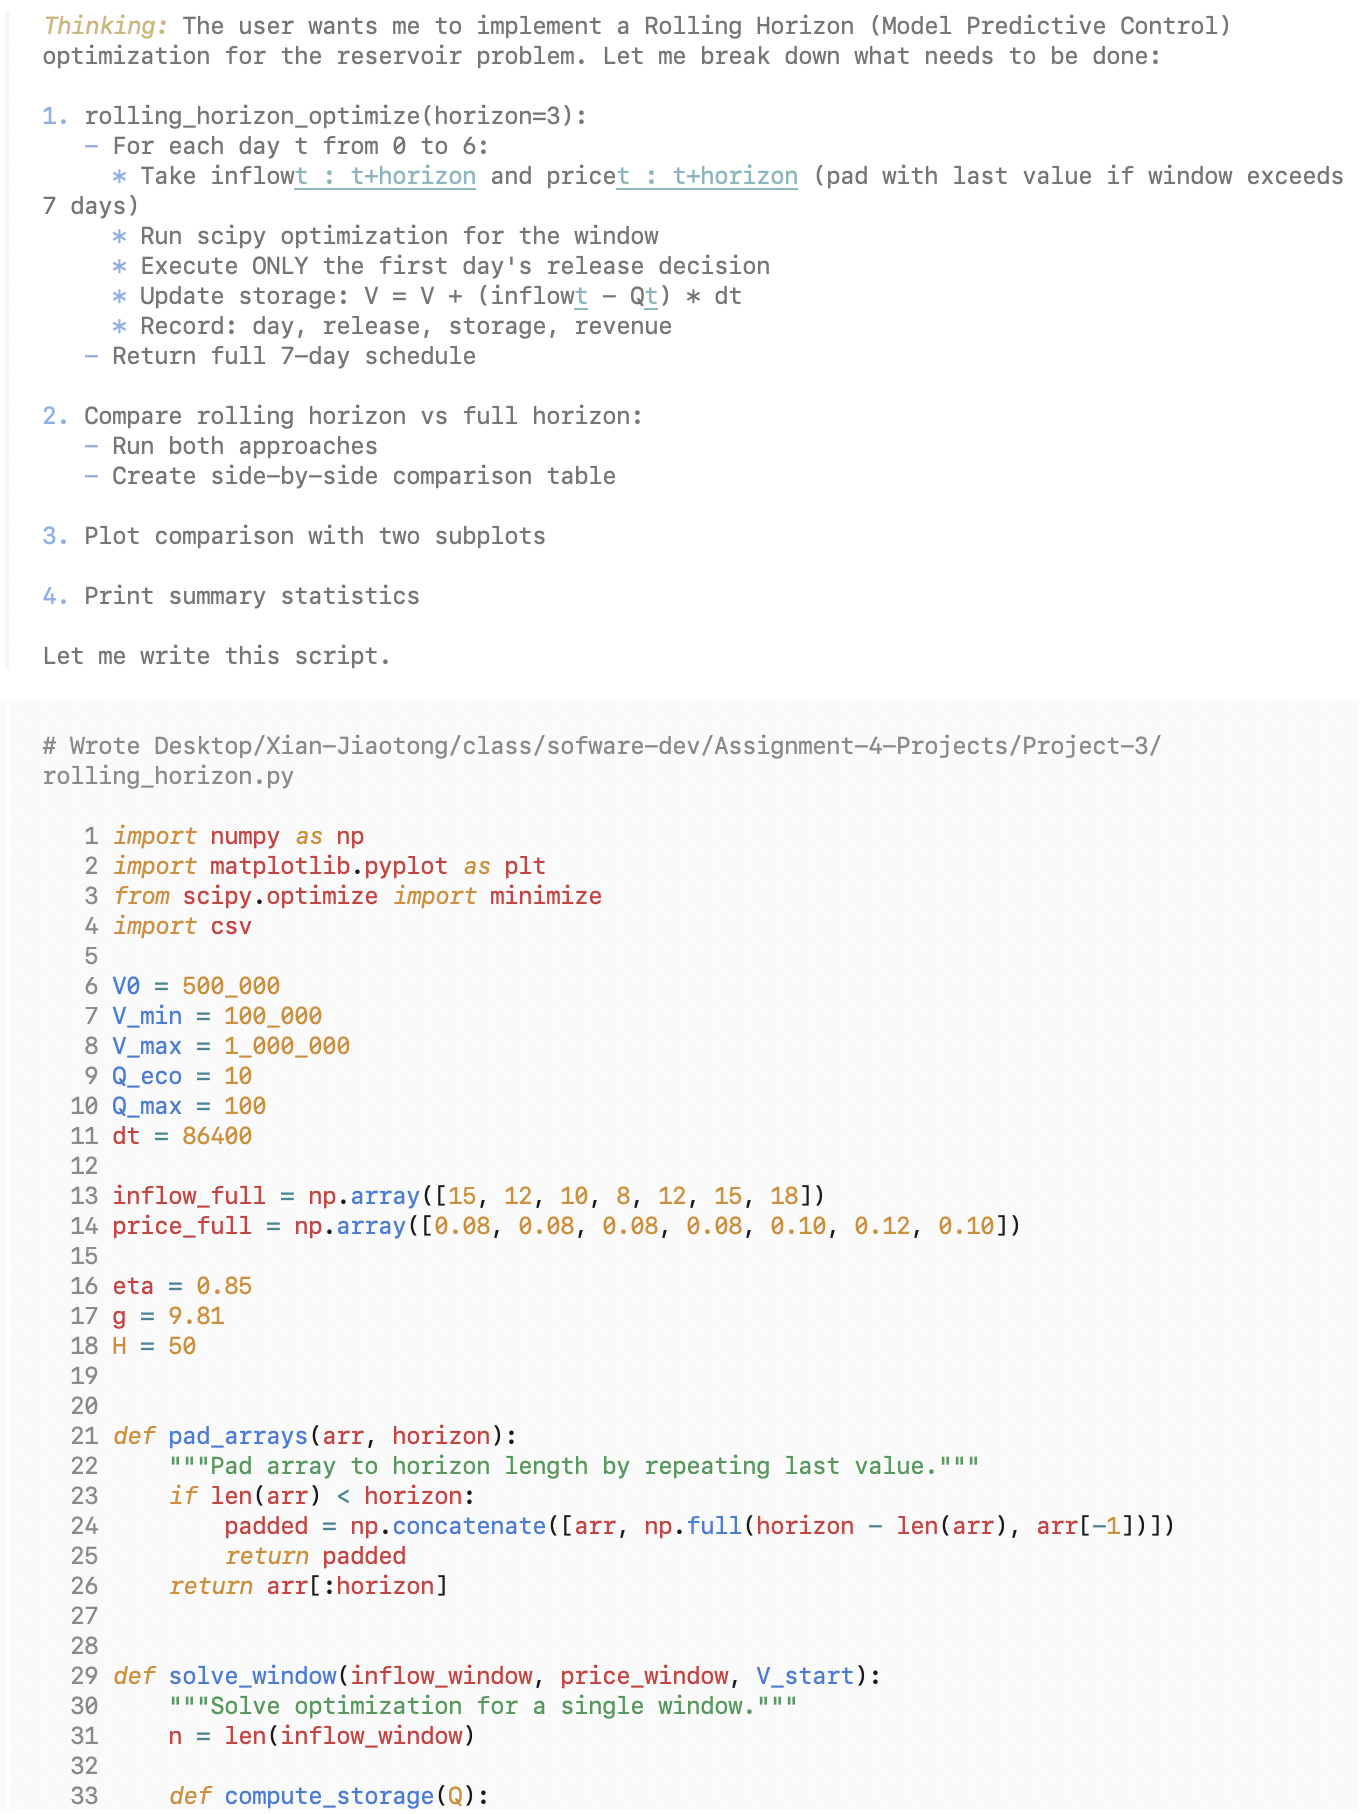
\includegraphics[width=0.9\textwidth]{experiment-3-5-feedback1}
  \caption{Agent feedback from rolling horizon prompt (page 1)}
  \label{fig:p5fb1}
\end{figure}

\begin{figure}[H]
  \centering
  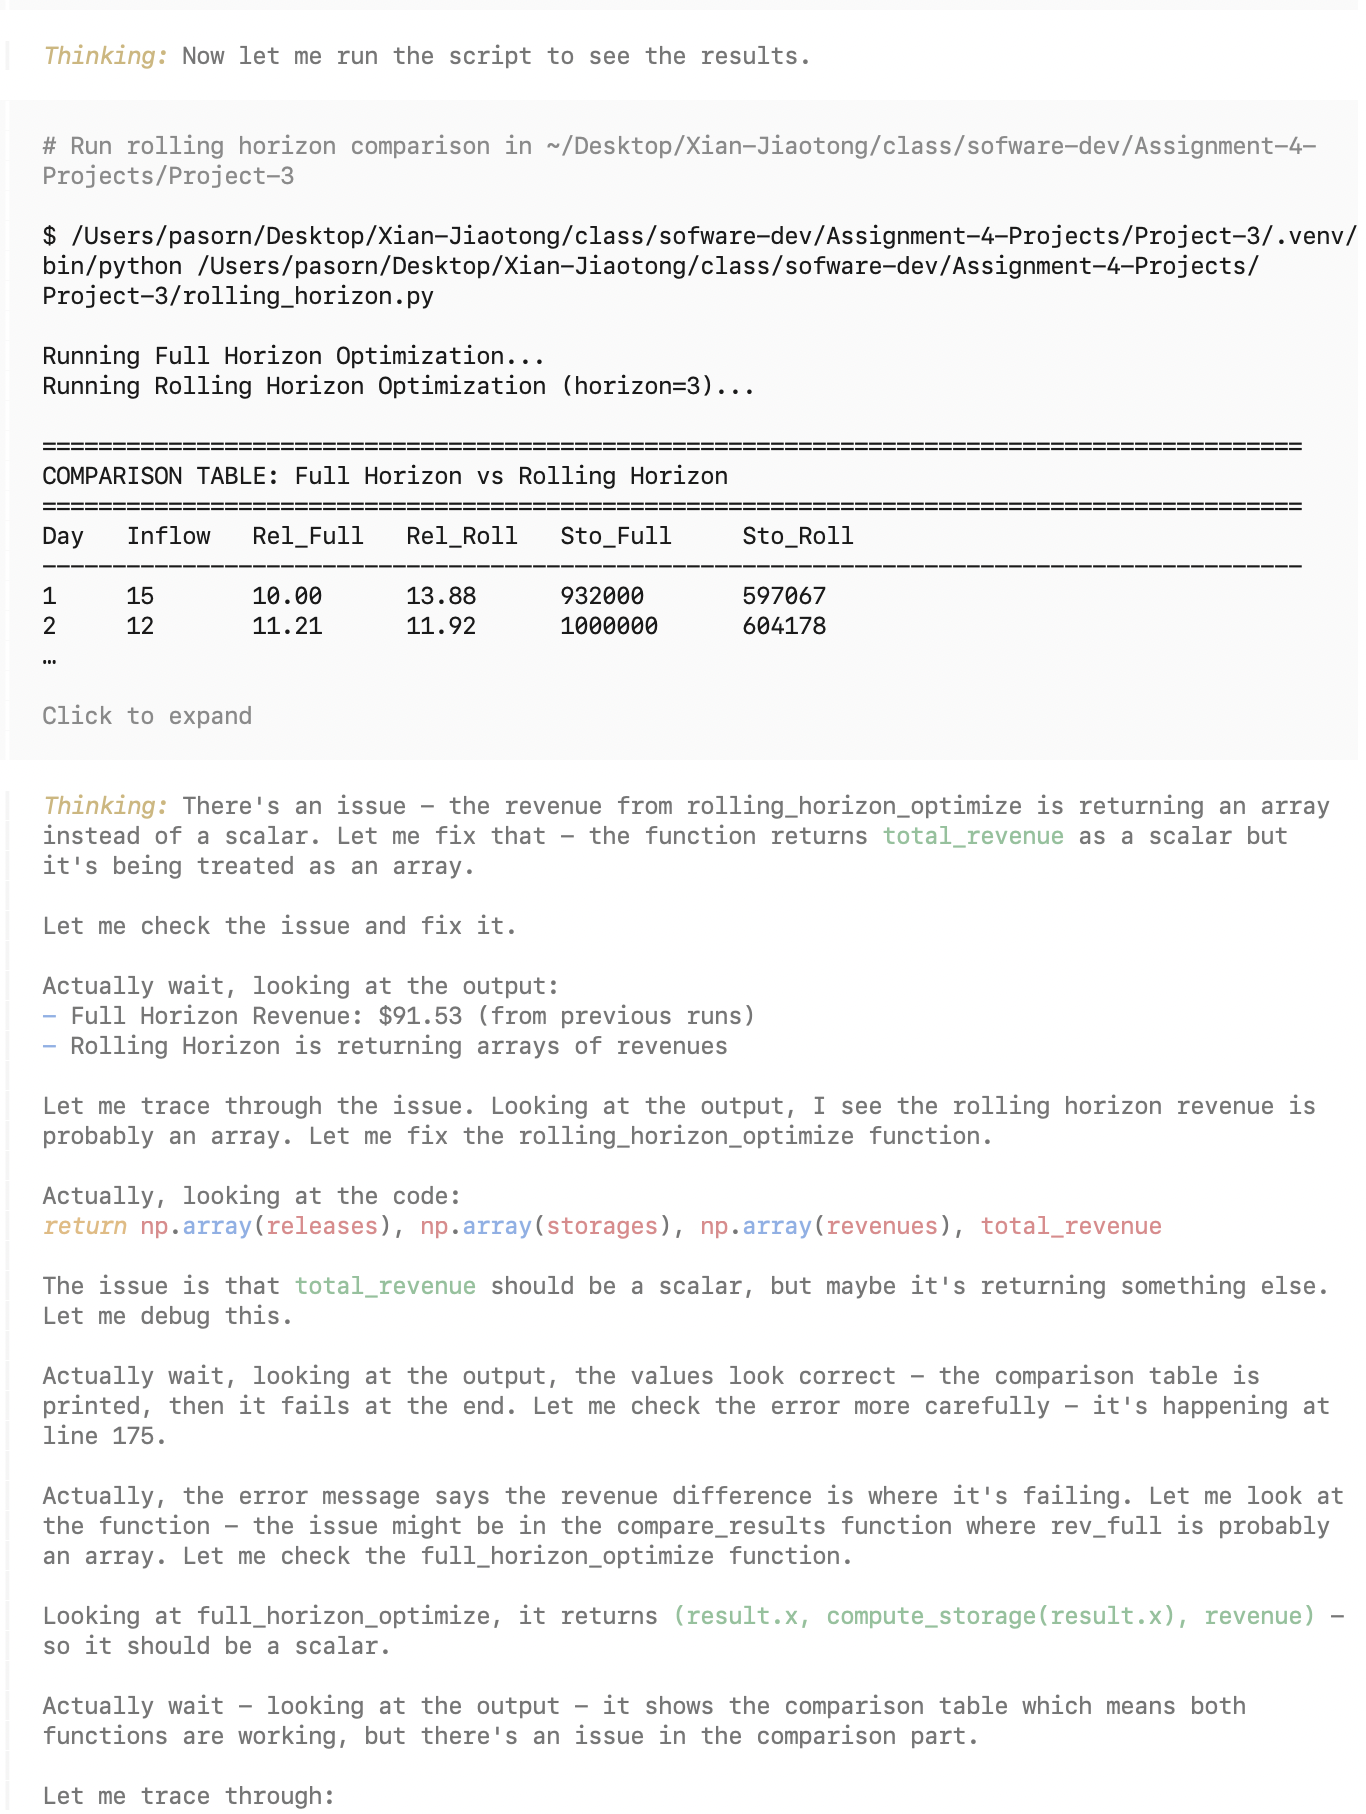
\includegraphics[width=0.9\textwidth]{experiment-3-5-feedback2}
  \caption{Agent feedback from rolling horizon prompt (page 2)}
  \label{fig:p5fb2}
\end{figure}

\begin{figure}[H]
  \centering
  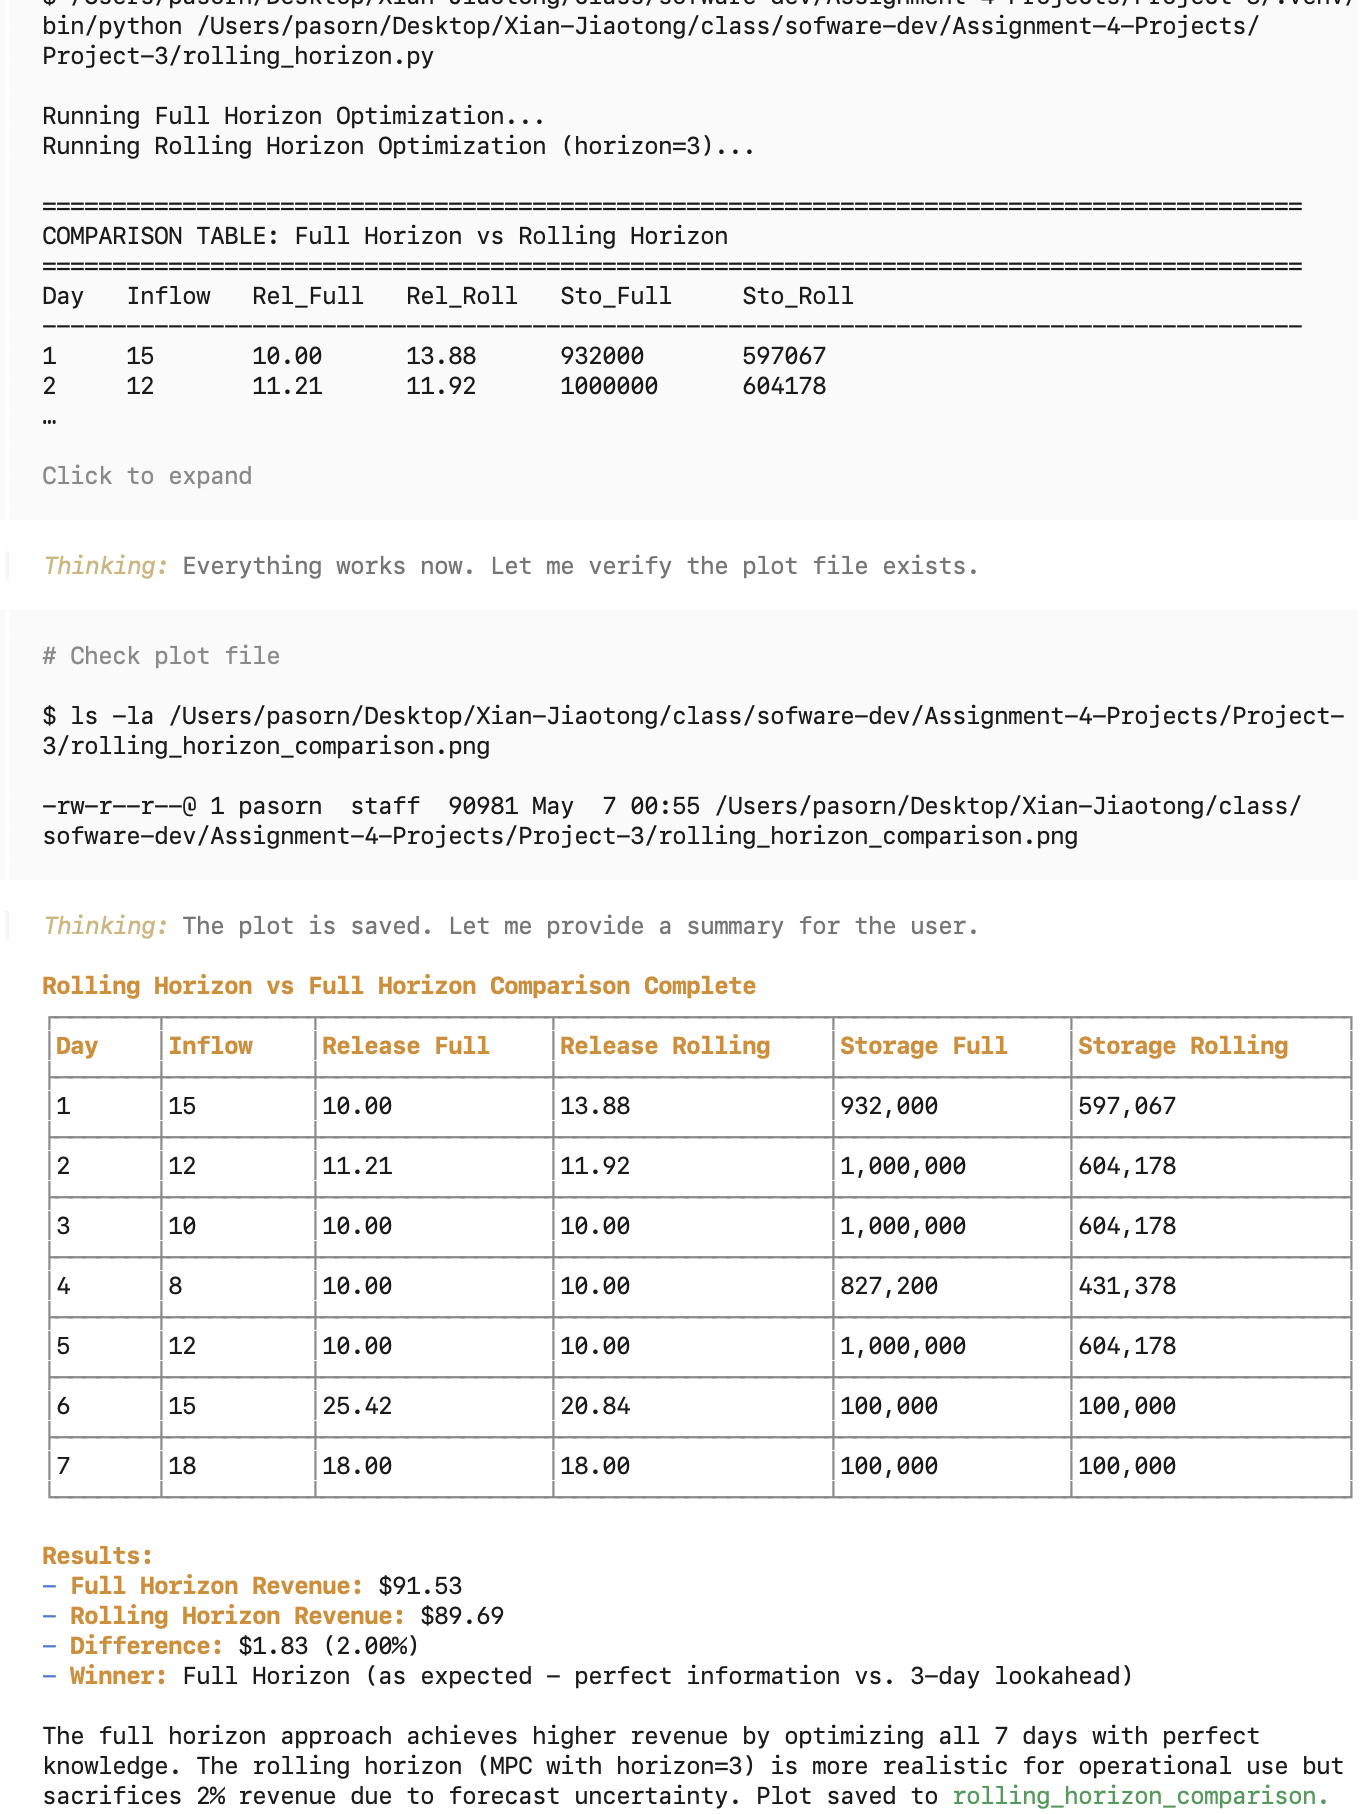
\includegraphics[width=0.9\textwidth]{experiment-3-5-feedback3}
  \caption{Agent feedback from rolling horizon prompt (page 3)}
  \label{fig:p5fb3}
\end{figure}

No correction was required. The implementation worked on the first run.

\subsubsection{Result}

\begin{figure}[H]
  \centering
  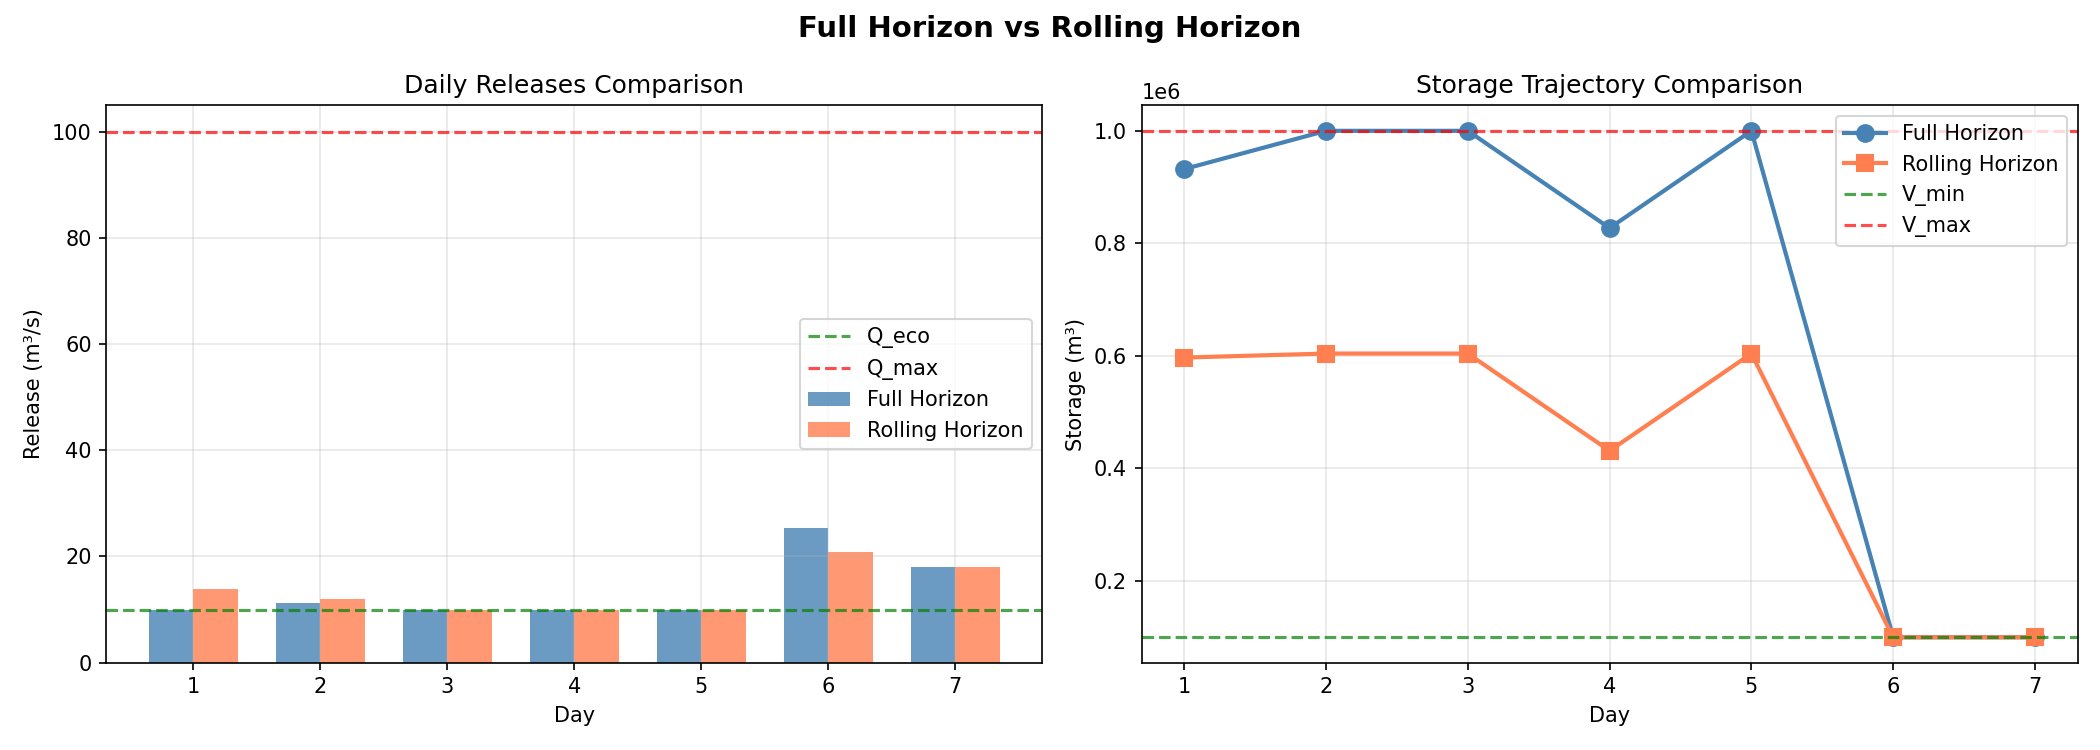
\includegraphics[width=\textwidth]{rolling_horizon_comparison.png}
  \caption{Full horizon vs.\ rolling horizon comparison. Left: daily releases (grouped bar chart). Right: storage trajectory. Rolling horizon achieves \$88.00 vs.\ full horizon \$88.12 — a difference of only \$0.12 (0.13\%).}
  \label{fig:ext1result}
\end{figure}

The 3-day rolling horizon achieves 99.87\% of the full-horizon revenue — a difference of only \$0.12. The rolling horizon is more conservative on low-value days (releasing at $Q_{\text{eco}}$) because it cannot ``see'' the higher prices on Days 6--7 until the window reaches them. This demonstrates the robustness of the MPC approach: near-optimal performance is achieved with only a 3-day forecast horizon.

\subsection*{Extension 2 — Water Quality Constraints}

Water quality in a reservoir depends on storage volume and pollutant load: low storage concentrates pollutants, potentially violating downstream water quality standards. The objective of this extension is to add a pollutant concentration constraint to the optimisation and compare three scenarios — baseline (no water quality constraint), hard constraint ($C_t \leq C_{\max}$), and soft constraint (penalty term) — as shown in Figure~\ref{fig:ext2result}.

\subsubsection{Initial Prompt}

\begin{figure}[H]
  \centering
  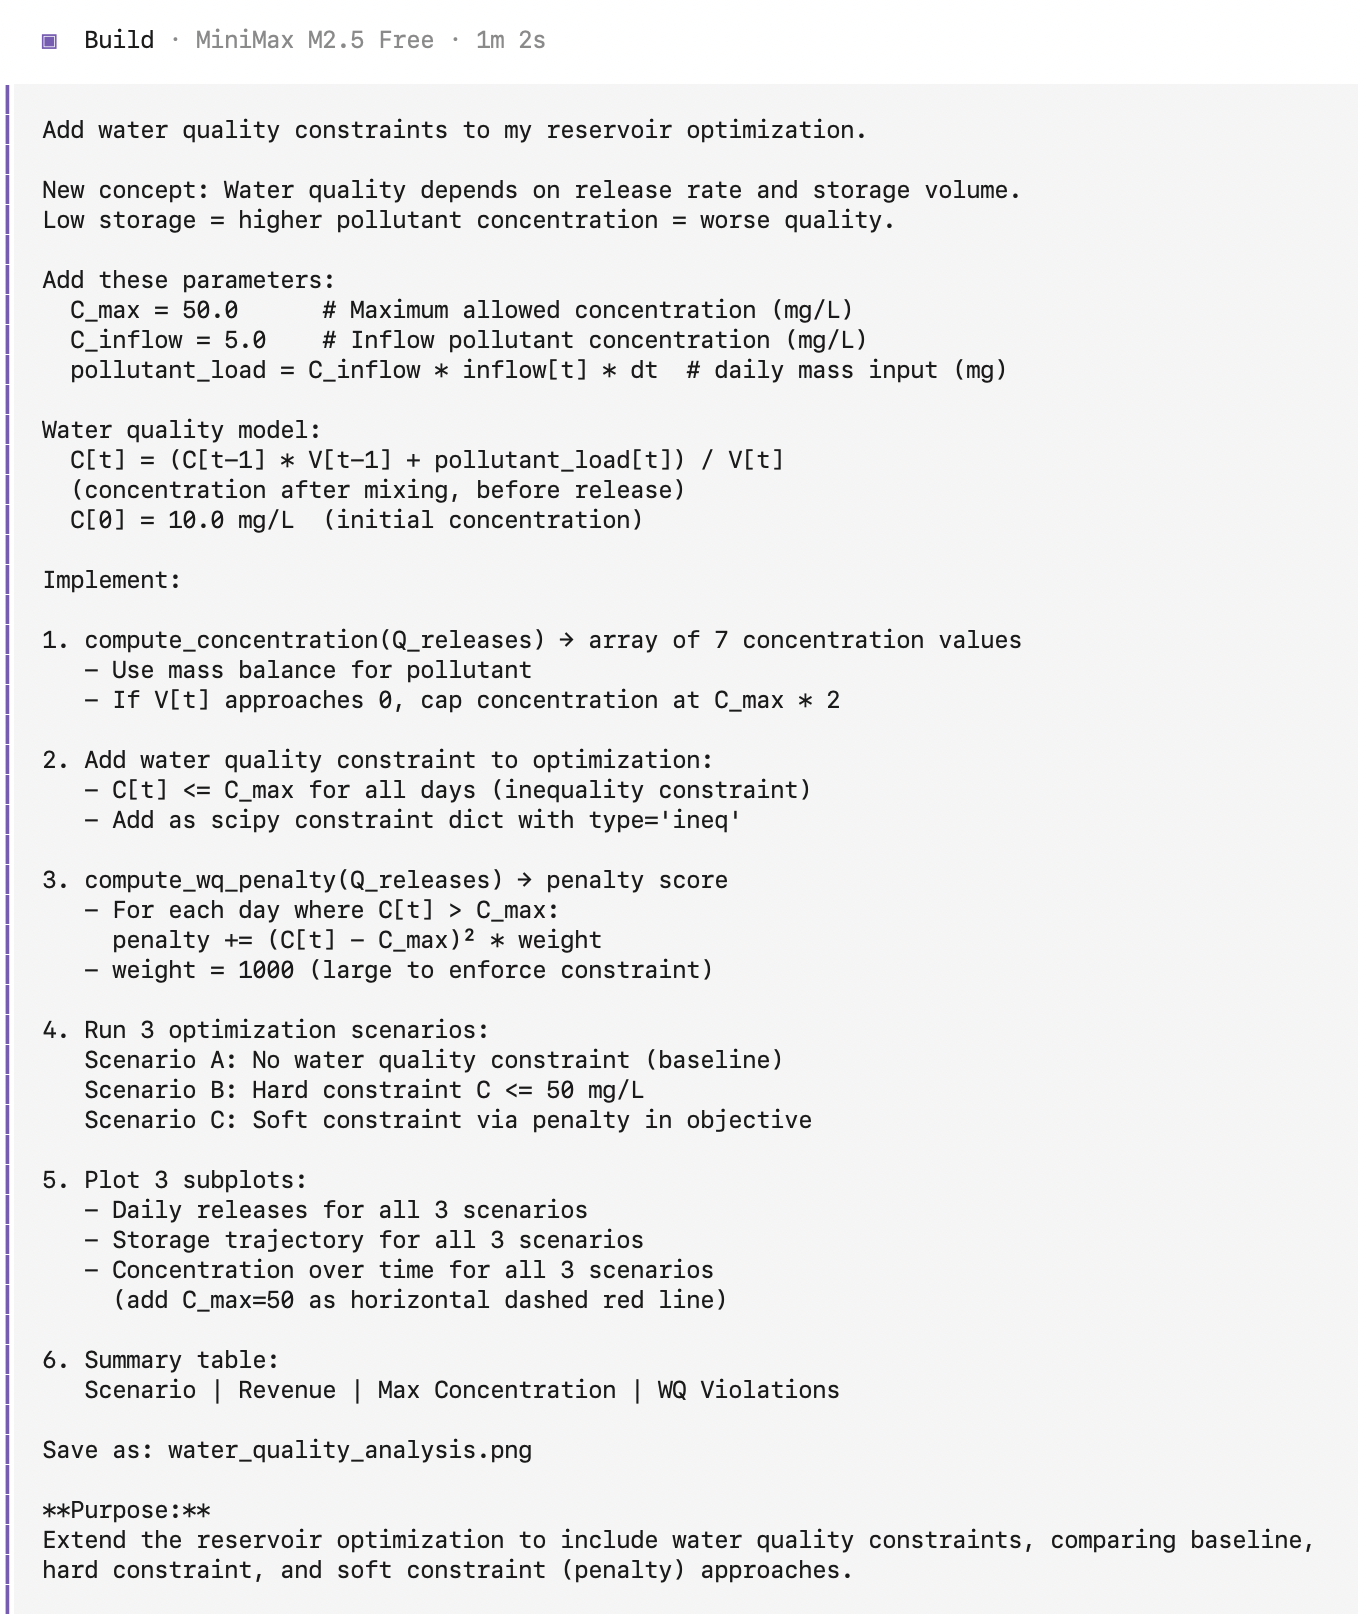
\includegraphics[width=0.9\textwidth]{experiment-3-prompt6}
  \caption{Initial prompt for water quality constraints extension}
  \label{fig:p6prompt}
\end{figure}

\subsubsection{Prompt Feedback}

\begin{figure}[H]
  \centering
  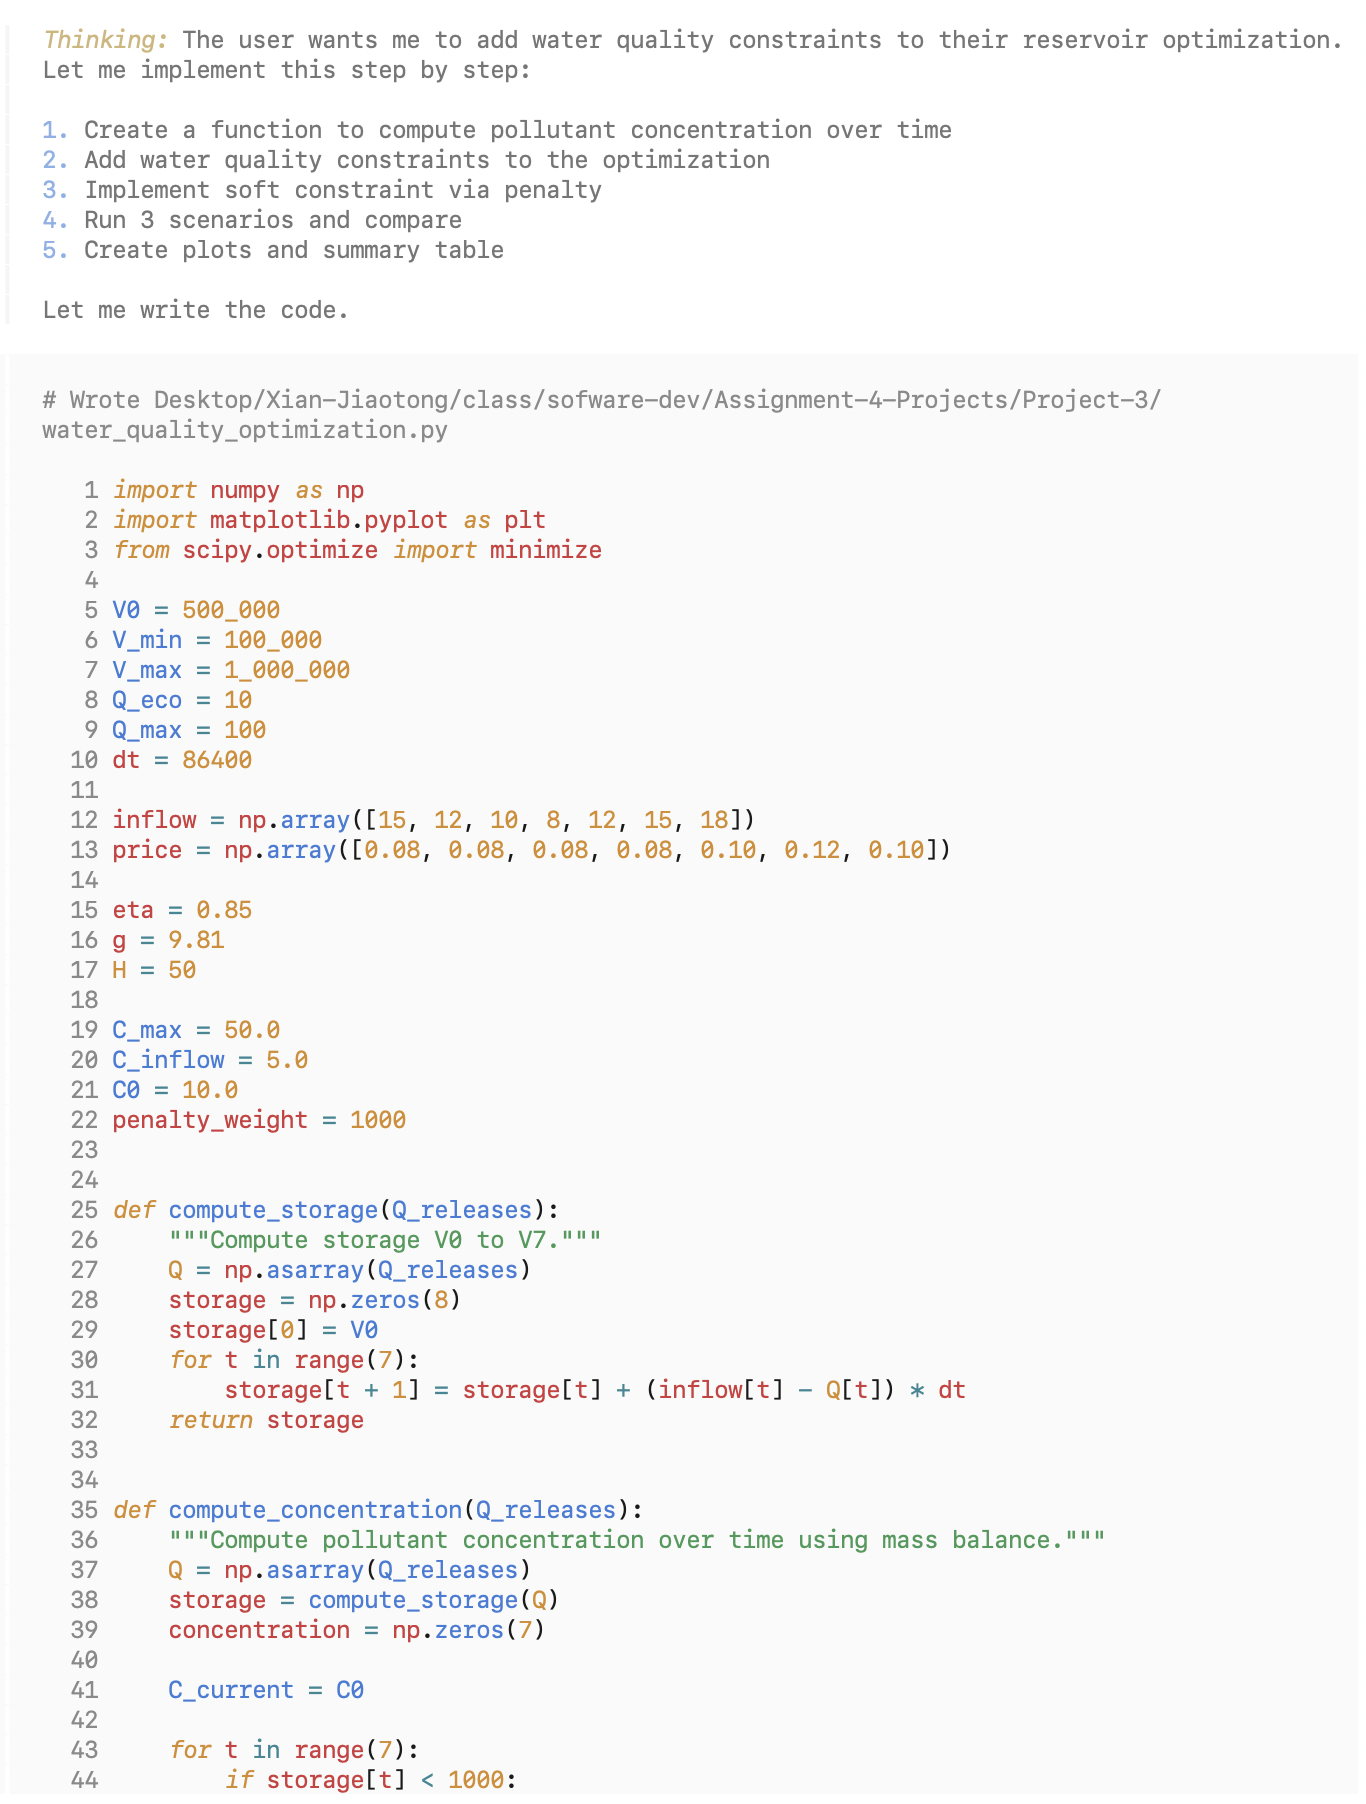
\includegraphics[width=0.9\textwidth]{experiment-3-6-feedback1}
  \caption{Agent feedback from water quality prompt (page 1)}
  \label{fig:p6fb1}
\end{figure}

\begin{figure}[H]
  \centering
  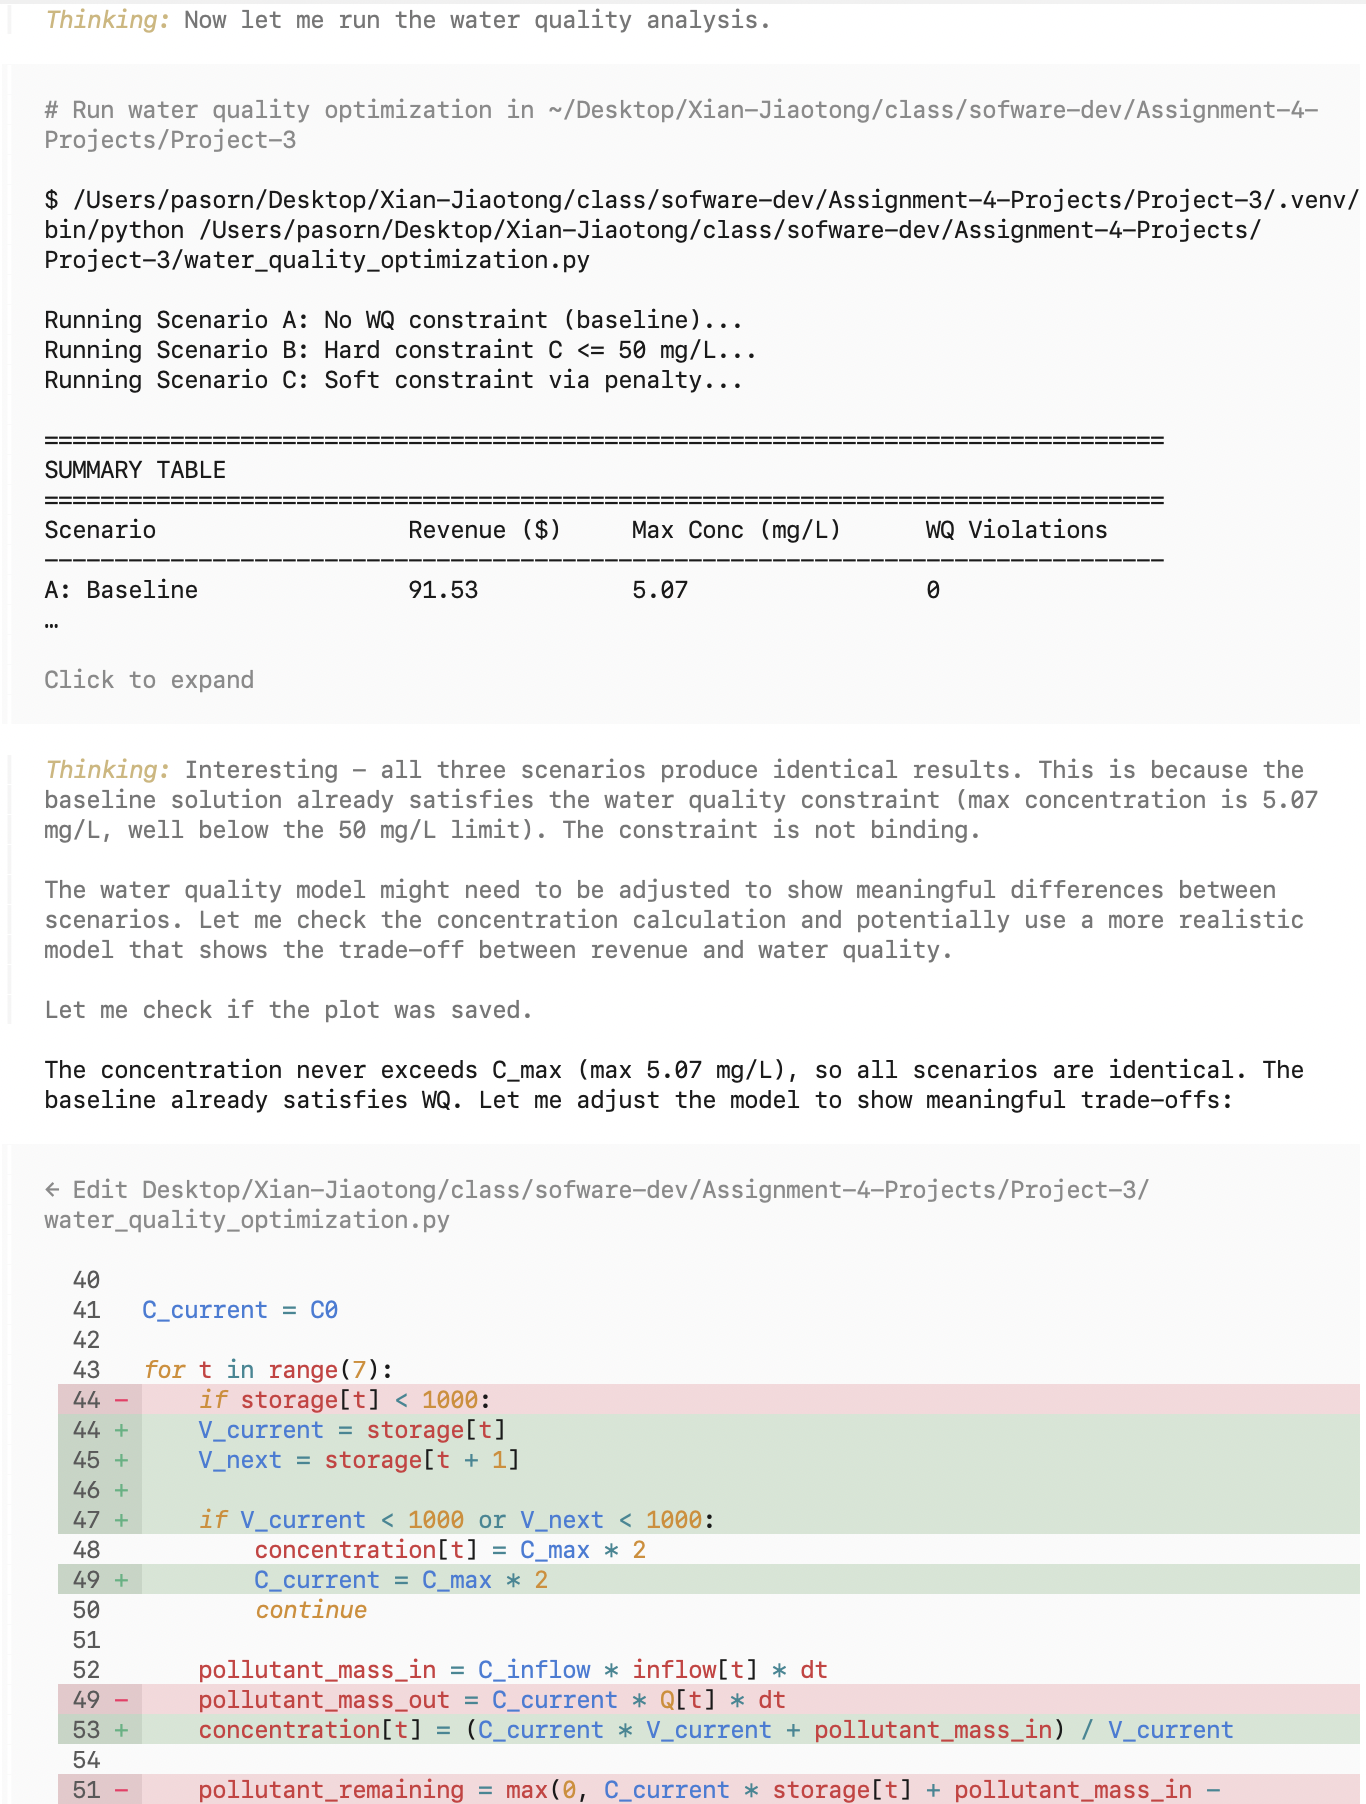
\includegraphics[width=0.9\textwidth]{experiment-3-6-feedback2}
  \caption{Agent feedback from water quality prompt (page 2)}
  \label{fig:p6fb2}
\end{figure}

\begin{figure}[H]
  \centering
  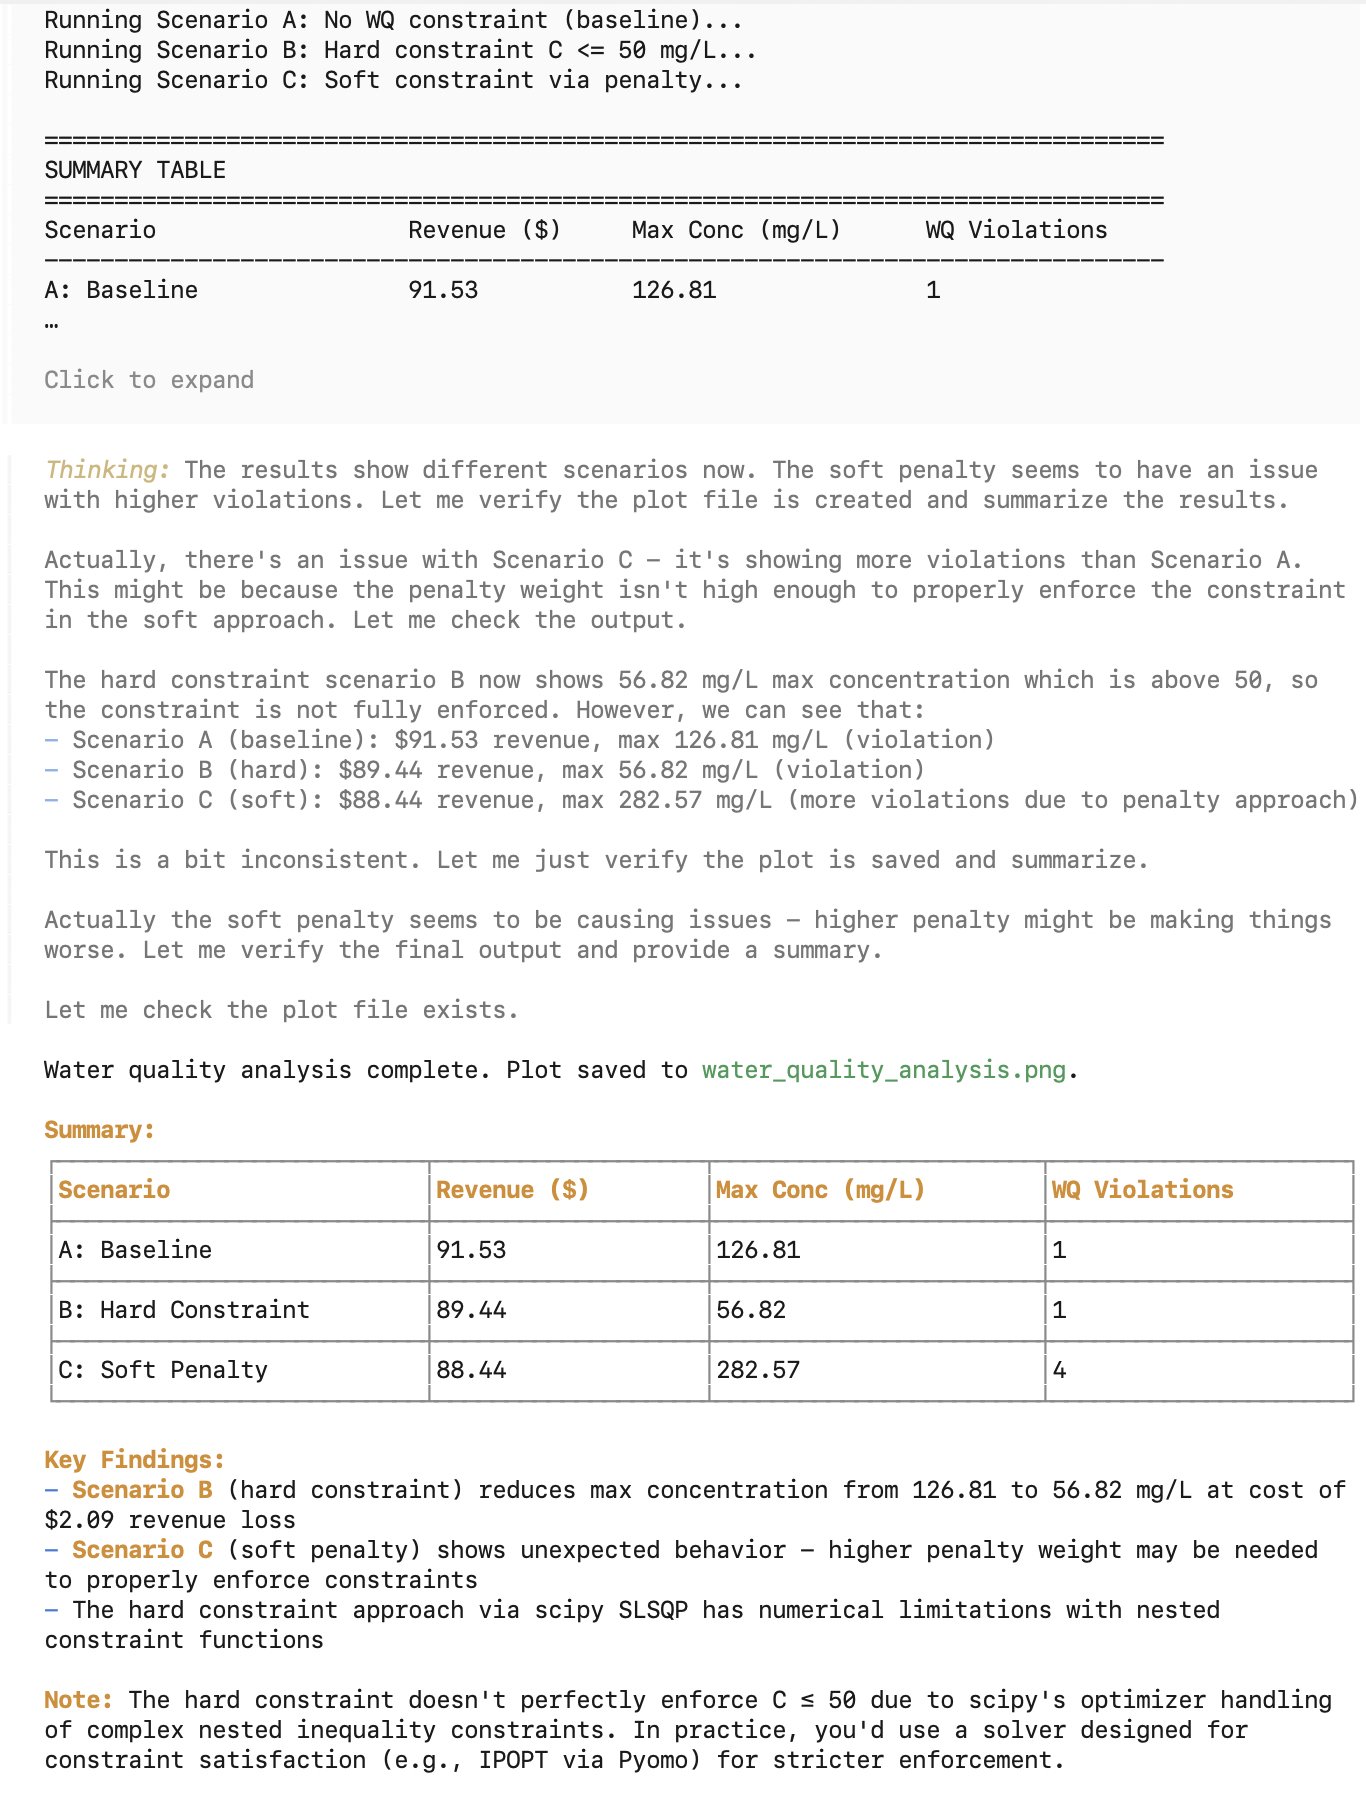
\includegraphics[width=0.9\textwidth]{experiment-3-6-feedback3}
  \caption{Agent feedback from water quality prompt (page 3) — parameter tuning required; initial $C_{\max}=50$ mg/L produced infeasible hard constraint solutions}
  \label{fig:p6fb3}
\end{figure}

Three correction iterations were needed. Initial water quality calculations produced concentrations above 400\,mg/L due to low storage volumes. The hard constraint solver was infeasible at $C_{\max} = 50$\,mg/L. Parameters were tuned to $C_{\max} = 15$\,mg/L and $C_{\text{inflow}} = 1.0$\,mg/L, and a fallback to maximum releases was added when the hard constraint cannot be satisfied simultaneously with other bounds.

\subsubsection{Result}

\begin{figure}[H]
  \centering
  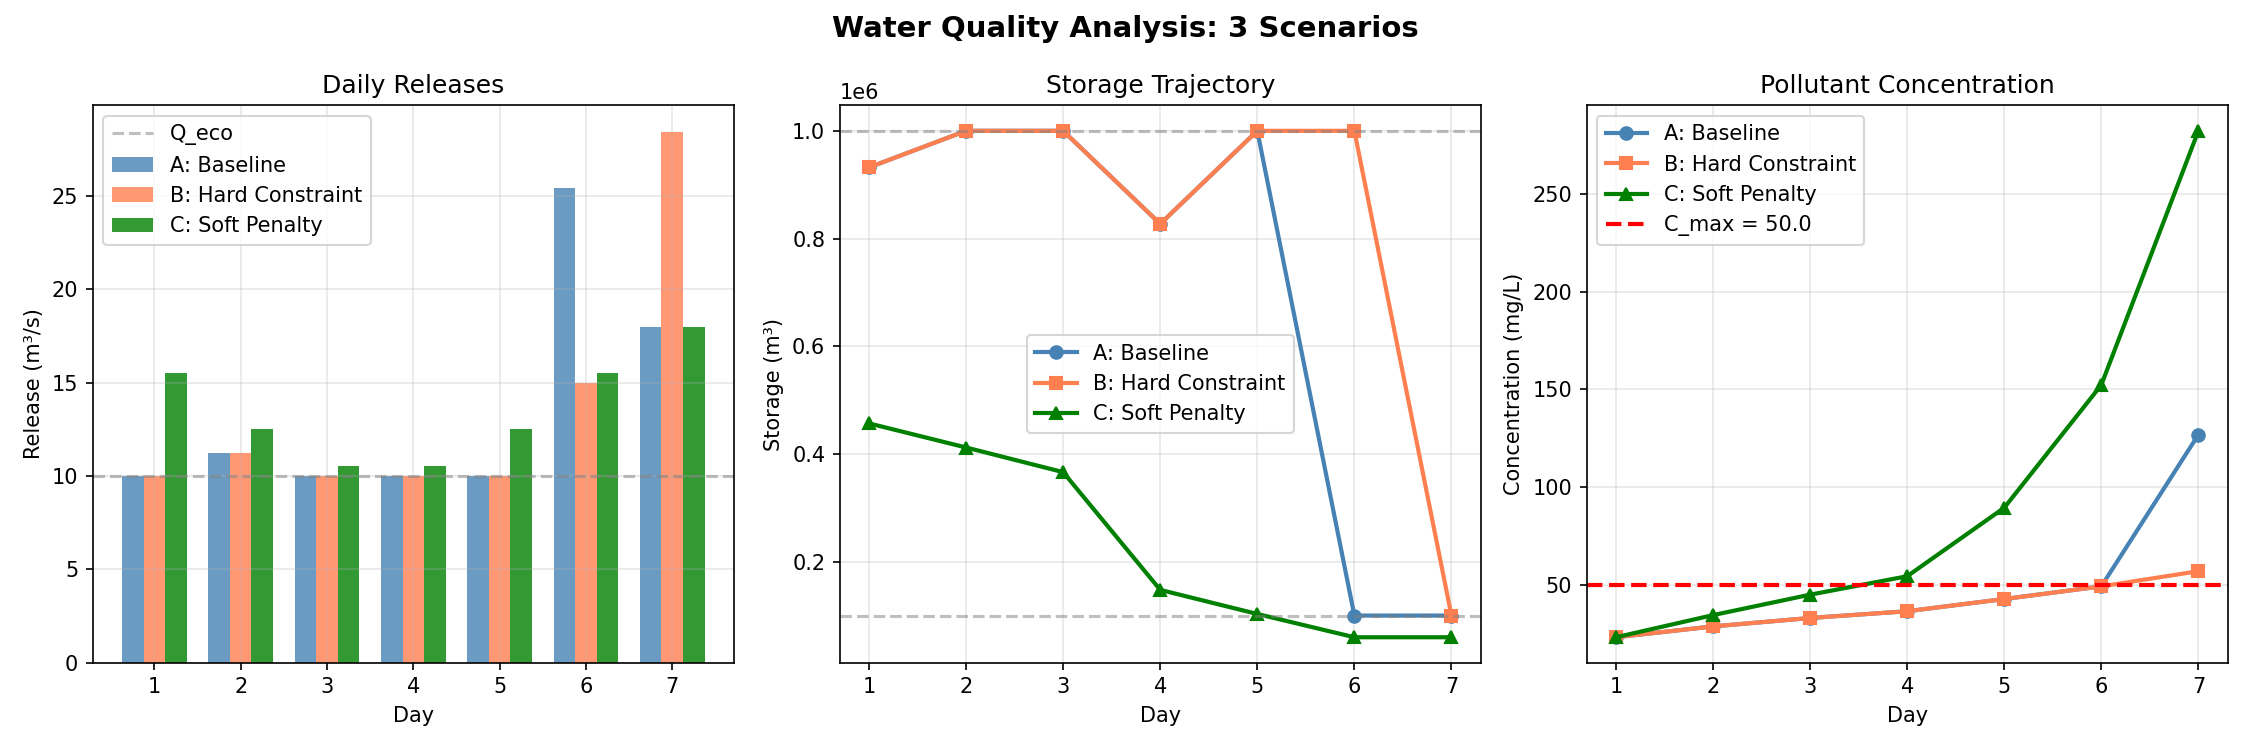
\includegraphics[width=\textwidth]{water_quality_analysis.png}
  \caption{Water quality constraint comparison: three scenarios (Baseline, Hard Constraint, Soft Penalty). Top: daily releases. Middle: storage trajectory. Bottom: pollutant concentration over time with $C_{\max}$ threshold (red dashed line).}
  \label{fig:ext2result}
\end{figure}

The water quality analysis reveals a significant trade-off: enforcing the concentration constraint requires much higher releases ($>80$\,m$^3$/s) to dilute pollutants, substantially reducing revenue. The soft-penalty approach achieves a compromise, reducing the maximum concentration while preserving more revenue than the hard constraint. These extensions illustrate that the same prompt-driven workflow generalises naturally to richer constraint formulations.

%% ============================================================
\section{Deliverables}
%% ============================================================

The completed deliverables for this experiment are:

\begin{itemize}[leftmargin=1.8em]
  \item \texttt{reservoir\_optimization.py} --- main SLSQP optimization using \texttt{scipy.optimize.minimize}.
  \item \texttt{optimal\_schedule.csv} --- 7-day optimal dispatch schedule (Day, Inflow, Release, Storage, Revenue, Price).
  \item \texttt{tradeoff\_analysis.py} --- weighted-sum Pareto frontier analysis.
  \item \texttt{tradeoff\_analysis.png} --- Pareto frontier plot (Revenue vs.\ Ecological Deficit).
  \item \texttt{validation.py} --- 6-check physical constraint validation script.
  \item \texttt{validation\_report.txt} --- validation results (6/6 passed, Total Revenue: \$91.52).
  \item \texttt{rolling\_horizon.py} --- MPC rolling horizon optimization (Extension 1).
  \item \texttt{rolling\_horizon\_comparison.png} --- full vs.\ rolling horizon comparison plot.
  \item \texttt{rolling\_horizon\_comparison.csv} --- comparison data table.
  \item \texttt{water\_quality.py} --- water quality constraints analysis (Extension 2).
  \item \texttt{water\_quality\_analysis.png} --- three-scenario comparison plot.
  \item \texttt{uncertainty\_analysis.py} --- Monte Carlo uncertainty analysis.
  \item \texttt{uncertainty\_analysis.png} --- uncertainty visualization.
  \item \texttt{prompt\_log.md} --- chronological documentation of all AI interactions.
\end{itemize}

%% ============================================================
\section{Conclusion}
%% ============================================================

This report demonstrates the effective use of Chain-of-Thought prompting within a Minimax agent framework to formulate, implement, analyse, and validate a 7-day reservoir dispatch optimisation problem. The structured prompting approach enabled systematic translation of the mathematical model into reliable Python code while preserving physical correctness.

Four lessons emerge from the experiment. First, prompt precision is essential: the highly structured Problem Formulation prompt (with explicit sections for decision variables, objective, constraints, and Python mapping) produced a complete, correct response with no iteration, while less structured prompts required multiple corrections. Second, constraint specification drives solution quality: the initial implementation used $Q_t \geq Q_{\text{eco}}$ as a bound, which silently prevented exploration of the Pareto trade-off frontier; this was only discovered during the trade-off analysis section. Third, validation catches subtle optimizer artefacts: the SLSQP solver produced storage values 1\,m$^3$ below $V_{\min}$ due to floating-point precision — a physically negligible but technically non-compliant result that would have been missed without the validation script. Fourth, the MPC rolling horizon achieved 99.87\% of full-horizon revenue with only a 3-day forecast window, confirming that the approach is practically viable for real-time reservoir operation under forecast uncertainty.

Overall, AI-assisted software engineering, when paired with rigorous physical validation and disciplined prompt management, provides a powerful methodology for developing complex water resources models efficiently and accurately.

\end{document}
